\documentclass[msc]{mestrado}

\usepackage{master}

%% Inicio do documento
\begin{document}
\mainmatter

%\listoffigures

\headsep=30pt
\oddsidemargin=20pt
\begin{spacing}{1.14}
\parskip=3pt

%\chapter{Introdu��o}

%\chapter{Ethernet e Tempo Real}
\label{cap:motivacao} \label{sec:CSMACD}

%\chapter{O Protocolo \doris{}} % (10 pag)
\label{cap:doris} \label{sec:consVar}

\label{fig:dorisStruct}

%\chapter{Plataforma Operacional}
\label{cap:platOp} \label{sec:interrupt} \label{sec:experimentos}



\chapter{Ambiente de implementa��o e configura��o de \doris}
\label{cap:implementacao}

\section{Introdu��o}
\label{sec:introImp}

Neste cap�tulo, a implementa��o do protocolo de c�digo aberto \doriss � apresentada.
A plataforma de tempo real escolhida foi o sistema operacional de prop�sito geral
Linux, vers�o 2.6.19.7, dotado do \ing{patch} Xenomai, vers�o 2.4-rc5 e do
\nanokernell Adeos correspondente. Esta plataforma ser� simplesmente chamada
``Xenomai'' daqui para frente.  Como foi visto no cap�tulo \ref{cap:platOp}, Xenomai
oferece garantias temporais da ordem de dezenas de micro-segundos (nos equipamentos
utilizados no nosso laborat�rio), suficiente para a implementa��o de \doris.  Al�m
destas garantias temporais, a escolha do Xenomai apresenta duas vantagens
significativas. Em primeiro lugar, Xenomai oferece uma interface de programa��o
chamada RTDM (\ing{Real Time Driver Model}) cujo objetivo � unificar as interfaces
dispon�veis para programar controladores de dispositivos em plataformas de tempo
real baseadas em Linux~\cite{Kiszka05a}. O uso da interface RTDM garante, portanto, a
portabilidade do protocolo nestes outros ambientes de tempo real. Em segundo lugar,
Xenomai j� disp�e de um servi�o de comunica��o Ethernet, baseado na interface
RTDM. Esta camada, chamada RTnet \cite{Kiszka05b}, disponibiliza controladores de
placas de rede portados para o Xenomai, assim como um protocolo de comunica��o
Ethernet baseado em TDMA. Portanto, o trabalho de implementa��o do protocolo \doriss
p�de aproveitar estes componentes e as suas implementa��es, possibilitando a concentra��o
de esfor�os no desenvolvimento dos componentes espec�ficos de \doris.

O presente cap�tulo � organizado da seguinte maneira.  Inicialmente, uma descri��o
da pilha de rede do Linux � apresentada na se��o \ref{sec:redeLinux}.  Em seguida, a
camada de rede RTnet e sua interface RTDM com a plataforma Xenomai s�o descritos na
se��o \ref{sec:xenoRTnet}.  A se��o \ref{sec:dorisDisc} � dedicada � apresenta��o da
implementa��o de \doriss e da sua integra��o na camada RTnet do Xenomai. No final
desta mesma se��o, alguns resultados s�o apresentados. Por fim, algumas
conclus�es s�o discutidas na se��o~\ref{sec:impConc}.


\section{As camadas de rede e enlace do Linux}
\label{sec:redeLinux}

Esta se��o apresenta apenas alguns elementos da implementa��o, pelo \kernell Linux,
dos protocolos IP na camada de rede e Ethernet 802.3 na camada de enlace, pois
somente estas duas camadas s�o utilizadas pela implementa��o de \doris.  Estas duas
camadas utiliza principalmente duas estruturas para armazenar os dados necess�rios �
transmiss�o e recep��o de pacotes. A primeira, chamada \netdev, � associada ao
dispositivo da placa de rede. Esta estrutura utiliza apontadores de fun��es para
definir a interface entre o \kernell e as aplica��es. Vale mencionar, por exemplo,
as fun��es de acesso � mem�ria circular definida na zona DMA (\ing{Direct Memory
  Access}) utilizadas pelo controlador da placa de rede para armazenar os pacotes
sendo transmitidos e recebidos.  A implementa��o das fun��es da estrutura \netdevv
pelos controladores de dispositivos � necess�ria para que o \kernell possa
disponibilizar os servi�os associados a um \ing{hardware} espec�fico.

A segunda estrutura, chamada \skbb (de \ing{socket buffer}), cont�m as informa��es
associadas a um pacote de dados que s�o necess�rias ao seu encaminhamento nas
diferentes camadas do \kernel. Dentre as principais informa��es, podem ser citadas a
�rea da mem�ria onde os dados est�o armazenados, as eventuais informa��es de
fragmenta��o, e os diferentes cabe�alhos do pacote.

Quando um pacote � recebido na mem�ria local da placa de rede, o dispositivo copia
o pacote na mem�ria DMA prevista para este efeito. Para fins de otimiza��o, o
dispositivo pode ser configurado para operar com v�rios pacotes, ao inv�s de apenas
um.  Tal procedimento n�o muda o modo de opera��o, pois tratar v�rios pacotes de uma
vez � equivalente a tratar um pacote de tamanho maior. Portanto, ilustra-se-�
aqui o processo de recep��o de apenas um pacote.  Logo que o pacote se torna
dispon�vel na mem�ria DMA, o \kernell precisa ser informado da sua presen�a e da
necessidade de process�-lo.  Para este efeito, duas abordagens principais devem ser
mencionadas.

A primeira � baseada em interrup��es do processador. Assim que o controlador da
placa de rede termina a opera��o de DMA, o dispositivo da placa de rede interrompe o
processador para inform�-lo da presen�a do pacote a ser recebido. No tratador desta
interrup��o, o \kernell armazena as informa��es relevantes para localizar o pacote e
cria um \cod{softirq} (ver se��o \ref{sec:interrupt}) para executar as demais
opera��es necess�rias. Antes de retornar, o tratador habilita as interrup��es
novamente para permitir a recep��o de um novo pacote. Na aus�ncia de uma nova
interrup��o, o \cod{softirq} � escalonado imediatamente e executa basicamente as
seguintes opera��es: (i) aloca��o din�mica do espa�o de mem�ria de um \skb; (ii)
c�pia do pacote armazenado na mem�ria DMA neste \skb; e (iii) encaminhamento do
\skbb (via apontadores) para a camada IP.  Esta abordagem tem a seguinte
limita��o. Quando a taxa de chegadas de pacotes alcan�a um certo patamar, a chegada
de um novo pacote acontece antes que o tratador do pacote anterior termine de
executar. � medida que este cen�rio se repete, a fila de interrup��o em espera
aumenta, resultando num situa��o de \ing{livelock}, pois o tratamento das
interrup��es tem a maior prioridade no sistema. O processador fica, ent�o,
monopolizado sem que haja possibilidade alguma de executar os \cod{softirqs}
escalonados ou qualquer outro processo.  Em algum momento, a mem�ria DMA fica cheia
e novos pacotes s�o descartados.
 
A segunda abordagem, que resolve o problema do \ing{livelock}, � o m�todo chamado de
consulta (\ing{polling}), no qual o \kernell consulta periodicamente o dispositivo
da placa de rede para saber se h� algum pacote em espera para ser recebido. Se
este for o caso, o \kernell processa parte ou todos dos pacotes que estiverem
esperando.  Este segundo m�todo tem a vantagem de suprimir as interrup��es do
processador pela placa de rede. No entanto, a sua utiliza��o introduz uma sobrecarga
do processador quando n�o h� pacote chegando na placa de rede. Al�m disso, este
m�todo introduz uma certa lat�ncia para o tratamento dos pacotes. No pior caso, um
pacote chega logo depois da consulta da placa de rede pelo processador. Neste caso,
o pacote s� ser� processado depois de um per�odo de consulta.

Para evitar os defeitos e aproveitar as vantagens de ambos os m�todos, o
\kernell utiliza uma solu��o h�brida proposta por \cite{Salim01}. Esta solu��o,
chamada NAPI (Nova API), utiliza a possibilidade que o \kernell tem de desabilitar
as interrup��es de maneira seletiva, isto �, referentes a apenas um dispositivo espec�fico. Na
chegada de um pacote, a seguinte seq��ncia de eventos � executada:

\begin{enumerate}
\item o dispositivo copia o pacote na mem�ria circular DMA. Na aus�ncia de
  espa�o nesta mem�ria, o pacote pode ser tanto descartado quanto copiado no lugar
  do mais velho pacote j� presente na mem�ria local.;
\item se as interrup��es da placa de rede forem habilitadas, o dispositivo
  interrompe o processador para inform�-lo que h� pacote em espera na mem�ria
  DMA. Sen�o, o dispositivo continua a receber pacote e transferi-los para a mem�ria
  DMA, sem interromper o processador;
\item na ocorr�ncia de uma interrup��o da placa de rede, o tratador come�a por
  desabilitar as interrup��es provenientes deste dispositivo, antes de agendar um
  \cod{softirq} para consultar a placa de rede;
\item em algum momento futuro, o \kernell escalona o \cod{softirq} de consulta da
  placa de rede e processa parte ou todos os pacotes esperando na mem�ria DMA. Se o
  n�mero de pacotes para serem processados � maior que o limite configurado, o
  \cod{softirq} agenda-se para process�-los posteriormente. Em seguida, o \kernell
  executa outros \cod{softirqs} que est�o eventualmente em espera, antes de
  escalonar o \cod{softirq} de consulta da placa de rede novamente;
\item quando a mem�ria DMA n�o cont�m mais nenhum pacote, quer seja porque eles foram
  processados ou porque foram silenciosamente descartados, o \cod{softirq} habilita
  as interrup��es da placa de rede novamente antes de retornar.
\end{enumerate}

Como pode ser constatado, esta solu��o impede o cen�rio de \ing{livelock} gra�as �
desabilita��o seletiva das interrup��es. Por outro lado, a consulta da placa de rede
s� acontece quando pelo menos um pacote chegou, evitando portanto a sobrecarga
desnecess�ria do processador.

Do ponto da visto das lat�ncias, esta solu��o tem os seguintes defeitos. O
\cod{softirq} de consulta pode ser escalonado depois de um tempo n�o previs�vel, na
ocorr�ncia de outras interrup��es causadas por qualquer outro dispositivo. Durante a
sua execu��o, este \cod{softirq} deve alocar dinamicamente os espa�os de mem�rias
necess�rios (\skb) para armazenar os pacotes. Esta aloca��o pode tamb�m levar um
tempo imprevis�vel, pois a chamada de sistema \cod{malloc} pode falhar, na aus�ncia
de mem�ria dispon�vel.

As se��es a seguir mostram como estes problemas s�o resolvidos pela camada RTnet
da plataforma Xenomai.


\section{A camada de rede do Xenomai: RTnet}
\label{sec:xenoRTnet}

\subsection{RTDM}
\label{sec:RTDM}

Antes de apresentar o projeto RTnet em detalhes, precisa-se descrever brevemente a
interface de programa��o na qual ele se baseia, isto � a interface RTDM (\ing{Real
  Time Driver Model}) \cite{Kiszka05a}, que vem sendo desenvolvida pelo pr�prio Jan
Kiszka, principal autor do RTnet.

A API \ing{Real Time Driver Model} tem por objetivo oferecer uma interface de
programa��o unificada para sistemas operacionais de tempo real baseados em Linux. O
RTDM constitui uma camada de software que estende os controladores de dispositivos e
a camada de abstra��o do \ing{hardware} (HAL) para disponibilizar servi�os � camada de
aplica��o, conforme representado na figura \ref{fig:rtdm}.  O RTDM foi inicialmente
especificado e desenvolvido na plataforma Xenomai. No entanto, em vista dos
benef�cios trazidos por esta API, ela tamb�m foi adotada pelo RTAI.

\begin{figure}[bt]
  \vspace{0.5cm} \centering \input{fig/rtdm.pstex_t}
  \caption{A interface do RTDM (reproduzida de \cite{Kiszka05a})}
  \label{fig:rtdm}
\end{figure}

A interface do RTDM oferecida para as aplica��es pode ser dividida em dois conjuntos
de fun��es. O primeiro conjunto � constitu�do das fun��es que d�o suporte aos
dispositivos de entrada e sa�da e aos dispositivos associados � servi�os. O segundo
conjunto � constitu�do das fun��es associadas aos servi�os de tempo real b�sicos,
independentes do hardware.

\begin{itemize}
\item[] \act{Servi�os de entrada e sa�da e troca de mensagens} Para este conjunto de
  fun��es, o RTDM segue o modelo de entrada e sa�da e o padr�o de comunica��o via
  \ing{socket} do padr�o POSIX 1003.1~\cite{POSIX04}.  Os dispositivos de entrada e
  sa�da, tamb�m chamados de dispositivos nomeados, disponibilizam as suas
  funcionalidades atrav�s de um arquivo especial no diret�rio \cod{/dev}. Os
  dispositivos associados a protocolos, dedicados � troca de mensagens, registram os
  seus servi�os atrav�s da implementa��o de um conjunto de fun��es definidas pelo
  RTDM na estrutura \cod{rtdm\_device}. Exemplos de algumas destas fun��es s�o
  \cod{socket, bind, connect, send\_mesg, recv\_msg}. Para diferenciar tal fun��o
  das fun��es usuais do \kernel, o sufixo \cod{\_rt} ou \cod{\_nrt} � adicionado ao
  seu nome. Do ponto de vista das aplica��es, a API do RTDM utiliza os nomes do
  padr�o POSIX com o prefixo \cod{rt\_dev\_}. Desta forma, a correspond�ncia entre
  uma chamada e a fun��o para ser executada � realizada pelo Xenomai, de acordo com
  o contexto no qual a fun��o � chamada. Por exemplo, se o contexto for de tempo
  real, a chamada \cod{rt\_dev\_sendmsg} levar� a execu��o da fun��o
  \cod{sendmsg\_rt}. Caso contr�rio, a fun��o \cod{sendmsg\_nrt} ser� executada.
\item[] \act{Servi�os do \ing{nanokernel}} Este segundo conjunto de fun��es diz
  respeito � abstra��o dos servi�os do \nanokernell de tempo real. Elas contemplam
  notadamente os servi�os de rel�gios de alta precis�o e dos temporizadores
  associados, as opera��es associadas ao gerenciamento de tarefas, os servi�os de
  sincroniza��o e de gerenciamento das linhas de interrup��es, e um servi�o de
  sinaliza��o para permitir a comunica��o entre os diferentes dom�nios registrados
  no \ing{ipipe}. Al�m destes servi�os principais, v�rios outros utilit�rios s�o
  disponibilizados, tais como, a aloca��o din�mica de mem�ria e o acesso seguro ao
  espa�o de mem�ria usu�rio.
\end{itemize}

Deve ser observado que a API do RTDM tende a crescer rapidamente. Numa consulta ao
projeto Xenomai \cite{Xenomai} realizada em dezembro de 2007, enumerou-se um pouco
mais de 100 fun��es definidas por esta API. Desta forma, o uso do RTDM para a
implementa��o de \doriss apareceu como uma escolha interessante. Al�m disso,
o RTDM tamb�m � dispon�vel na plataforma RTAI, permitindo o uso dos produtos
de \ing{software} baseados nesta interface, tanto na plataforma Xenomai quanto no RTAI.


\subsection {A arquitetura do RTnet}
\label{sec:RTnet}

O projeto de c�digo aberto RTnet \cite{Kiszka05b} foi fundado em 2001 na
Universidade de Hannover com o objetivo de prover uma infraestrutura flex�vel e
independente do \ing{hardware} para servi�os de comunica��o de tempo real baseados em
Ethernet.  Desenvolvido inicialmente na plataforma de tempo real RTAI, este
projeto � tamb�m dispon�vel na plataforma Xenomai.

\begin{figure}[bt]
  \centering \input{fig/rtdmRTnet.pstex_t}
  \caption{Localiza��o do RTnet.}
  \label{fig:rtdmRTnet}
\end{figure}

A localiza��o do RTnet e das suas rela��es com as demais camadas do Xenomai �
representada na figura \ref{fig:rtdmRTnet}. Como pode ser observado, RTnet utiliza
os dispositivos de \ing{hardware} existentes e introduz uma camada de software para
aumentar o determinismo dos servi�os de comunica��o. Do ponto de vista da sua
interface com as aplica��es, RTnet utiliza o RTDM (\ing{Real Time Driver Model})
\cite{Kiszka05a}.  Em rela��o ao hardware, RTnet utiliza tanto a camada HAL, provida
pelo Xenomai, quanto controladores de dispositivos pr�prios. Para a implementa��o de
tais controladores, capazes de prover garantias temporais, o c�digo original dos
controladores de dispositivos do Linux � modificado, conforme a descri��o dispon�vel
na documenta��o do RTnet \cite{RTnet}.  O objetivo principal destas modifica��es �
remover do c�digo do dispositivo qualquer chamada �s fun��es bloqueantes do \kernell
Linux.

O detalhe dos componentes da pilha RTnet � apresentado na figura \ref{fig:RTnet}.
Como pode ser observado, RTnet se inspira na organiza��o em camada da pilha de rede
do Linux. No entanto, a implementa��o atual do RTnet s� oferece servi�os de
comunica��o baseados em UDP/IP e n�o fornece suporte ao protocolo TCP/IP.

\begin{figure}[bt]
  \vspace{0.5cm} \centering \input{fig/RTnet.pstex_t}
  \caption{Estrutura em camada do RTnet.}
  \label{fig:RTnet}
\end{figure}

Acompanhando a figura \ref{fig:RTnet} de cima para baixo, pode-se ver que os
servi�os oferecidos pelo RTnet utilizam a interface do RTDM para disponibilizar as
suas funcionalidades �s aplica��es. Uma interface espec�fica de configura��o,
atrav�s de fun��es \cod{ioctl}, � utilizada para as opera��es de
gerenciamento. Encaixados na interface abaixo do RTDM, os componentes da camada de
rede prov�em implementa��es espec�ficas dos protocolos UDP, ICMP, e ARP. A se��o
\ref{sec:UDPIP} mostra algumas das solu��es adotadas para aumentar o determinismo
dos protocolos UDP e ARP. O protocolo ICMP, baseado no protocolo IP, � dedicado �s
fun��es de controle e gerenciamento da rede. A sua implementa��o � bastante
espec�fica e de pouca relev�ncia para este trabalho, e portanto, n�o ser�
apresentada aqui.

Os componentes principais do RTnet s�o localizados abaixo da camada de rede e acima
dos controladores de dispositivos e da camada HAL. Eles constituem a camada RTmac e
o n�cleo RTnet ilustrados na figura \ref{fig:RTnet}. O n�cleo cont�m os servi�os de
emiss�o e recep��o dos pacotes, baseados na modifica��o dos controladores de
dispositivos. Detalhes desta implementa��o ser�o descritos na se��o
\ref{sec:princComp}.  Em rela��o ao RTmac, ele constitui uma caixa pronta na qual as
disciplinas de acesso ao meio s�o embutidas. Atrav�s da estrutura \cod{rtmac\_disc},
a interface RTmac indica as fun��es cuja implementa��o � necess�ria para definir
uma pol�tica de acesso ao meio. Na vers�o atual do RTnet, as duas disciplinas TDMA e
NoMAC s�o dispon�veis. Elas ser�o brevemente apresentadas, assim como a interface
RTmac, na se��o \ref{sec:discRTnet}.  O presente trabalho de implementa��o teve por
resultado a cria��o de uma nova disciplina de acesso ao meio, \doris, al�m das duas
disciplinas j� existentes.  Uma descri��o detalhada da implementa��o de \doriss ser�
realizada na se��o \ref{sec:dorisDisc}.

Al�m destes componentes principais, Rtnet providencia tamb�m servi�os de
configura��o (\texttt{RTcfg}) e de monitoramento (\texttt{RTcap}). Os primeiros
servem tanto para configurar a rede em tempo de projeto, quanto para modificar a
composi��o dos membros da rede de tempo real em tempo de execu��o. Os segundos
permitem coletar dados temporais sobre os pacotes transmitidos. Estes servi�os s�o
opcionais, e n�o ser�o descritos aqui.

Ao lado da pilha RTnet, aplica��es que utilizam os servi�os de melhor esfor�o da
pilha de rede do Linux podem faz�-lo atrav�s de interfaces virtuais, cujo mecanismo
ser� apresentado na se��o \ref{sec:princComp}, juntamente com a descri��o do
formato dos pacotes RTnet.

\subsection{RTnet: principais componentes}
\label{sec:princComp}

\subsubsection{Gerenciamento de mem�ria}

Foi visto na se��o \ref{sec:redeLinux} que a camada de rede do Linux aloca
dinamicamente um espa�o de mem�ria \skbb para armazenar um pacote durante a sua
exist�ncia na pilha de rede. Devido ao gerenciamento virtual da mem�ria, este pedido
de aloca��o de mem�ria pode resultar numa falta de p�gina. Neste caso, o processo
pedindo mem�ria � suspenso e o \kernell escalona o \ing{thread} respons�vel pelo
gerenciamento da mem�ria virtual para que ele libere algumas p�ginas n�o utilizadas
no momento. Este procedimento pode levar um tempo imprevis�vel, ou mesmo falhar em
alguma situa��o espec�fica.

Para evitar esta fonte de lat�ncia n�o determin�stica, RTnet utiliza um mecanismo de
aloca��o est�tica da mem�ria em tempo de configura��o. Nesta fase inicial, cada um
dos componentes da pilha, relativos aos processos de emiss�o ou recep��o, deve criar
uma reserva de estruturas \rtskb. Tal estrutura, similar � estrutura \skbb do Linux
padr�o, � utilizada para armazenar as informa��es e os dados de um pacote, desde sua
chegada na mem�ria DMA de recep��o, at� sua entrega � aplica��o destino. Cada
\rtskbb tem um tamanho fixo, suficiente para armazenar um pacote de tamanho
m�ximo. Como o tamanho de cada reserva de estruturas \rtskbb � fixo, um mecanismo de
troca � utilizado. Em outras palavras, para poder adquirir um \rtskbb de um
componente $A$, um componente $B$ deve dispor de um \rtskbb livre para dar em
troca. Observa-se que, como as estruturas s�o passadas por refer�ncias, tais
opera��es de troca s�o quase instant�neas em compara��o ao tempo que levaria a c�pia
do conte�do destas estruturas.
 

\subsubsection{Emiss�o e Recep��o de pacotes}
\label{sec:envRec}

A emiss�o de um pacote � uma opera��o que acontece no contexto da execu��o
seq�encial de um processo. Portanto, � um evento s�ncrono e as opera��es
subseq�entes s�o realizadas com a prioridade da tarefa que executa a opera��o de
emiss�o. Conseq�entemente, as garantias temporais associadas a uma emiss�o dependem
exclusivamente da plataforma operacional e da utiliza��o correta dos seus servi�os.

No caso da opera��o de recep��o de uma mensagem, a situa��o � diferente, pois esta
opera��o � um evento ass�ncrono. Em particular, n�o se sabe, no in�cio do
procedimento de recep��o, qual � a prioridade da aplica��o de destino do
pacote. Conseq�entemente, a tarefa de recep��o de pacote chamada ``gerente da
pilha'' (\ing{stack manager}) tem a maior prioridade no sistema. Desta forma,
garante-se que se o pacote for destinado a uma tarefa cr�tica, ele ser� encaminhado o
mais rapidamente poss�vel. O in�cio do processo de recep��o � parecido com este do
Linux (ver se��o \ref{sec:redeLinux}). Ap�s ter copiado um pacote na mem�ria DMA de
recep��o, a placa de rede interrompe o processador. Em seguida, o tratador da
interrup��o armazena o pacote numa estrutura \rtskbb da reserva do dispositivo e
coloca este \rtskbb numa fila de recep��o, antes de acordar o ``gerente da
pilha''. Este \ing{thread}, que come�a a executar imediatamente, pois tem a maior
prioridade do sistema, determina se o pacote � de tempo real ou n�o. Se for de tempo
real, ele efetua as opera��es de recep��o necess�rias at� entregar o pacote para a
aplica��o de destino. Caso contr�rio, o ``gerente'' coloca o pacote na fila dos
pacotes de melhor esfor�o para serem recebidos, acorda o processo de baixa
prioridade dedicado ao processamento desta fila e retorna.


\subsubsection{A camada de rede}
\label{sec:UDPIP}

Os principais problemas de lat�ncia para serem resolvidos na camada de rede s�o
devido ao uso do protocolo ARP (\ing{Address Resolution Protocol}) e aos mecanismos
de fragmenta��o de pacote do protocolo UDP/IP.

Em rela��o � fragmenta��o de pacote, o RTnet oferece uma op��o de configura��o que
permite transmitir pacotes de tamanho superior ao MTU de 1500 bytes do Ethernet
padr�o. As garantias de previsibilidade desta implementa��o s�o obtidas usando:
\begin{itemize}
\item reservas espec�ficas de estruturas \rtskbb para coletar os fragmentos de um
  mesmo pacote;
\item temporizadores associados a cada coletor para garantir o
  descarte de cadeias incompletas, antes que o conjunto de coletores
  se esgote. De fato, a perda de um pacote impede a complei��o da
  cadeia associada e impossibilita a libera��o da mem�ria utilizada
  por esta cadeia.
\end{itemize}

Al�m disso, esta implementa��o requer que os fragmentos de um mesmo pacote sejam
recebidos em ordem ascendente. Esta exig�ncia limita o uso da fragmenta��o �s redes
locais, nas quais a reordena��o de pacotes raramente acontece.

Em rela��o ao protocolo ARP, os protocolos de redes convencionais o utilizam
dinamicamente para construir a tabela ARP que associa os n�meros IP e os endere�os
de roteamento Ethernet \cite{Kurose05}. Para determinar o endere�o Ethernet
correspondente a um endere�o IP, uma esta��o envia um pacote ARP usando o endere�o
um-para-todos \linebreak(\cod{FF:FF:FF:FF:FF:FF}) do padr�o Ethernet, perguntando
quem det�m a rota para este IP. Se a m�quina de destino estiver no mesmo segmento
Ethernet, ela manda uma resposta informando o seu endere�o Ethernet. Caso contr�rio,
o roteador encarregado da sub-rede associada �quele IP informa do seu endere�o
Ethernet.  Quando a resposta chega, a tabela ARP da esta��o de origem �
atualizada. Para permitir a reconfigura��o autom�tica da rede, cada entrada desta
tabela � apagada periodicamente.
  
Este procedimento introduz uma fonte de lat�ncia no estabelecimento de uma
comunica��o entre duas esta��es, pois o tempo de resposta n�o � determin�stico, nem
a freq��ncia na qual a tabela ARP dever� ser atualizada. No caso do RTnet, este
procedimento foi trocado por uma configura��o est�tica da tabela ARP, realizada em
tempo de configura��o.
 

\subsubsection{Os pacotes RTnet}
\label{sec:pacoteRTnet}

Para manter a compatibilidade com os dispositivos de hardware, RTnet utiliza o
formato dos quadros Ethernet padr�o, com o cabe�alho de 14 bytes, incluindo os
endere�os de destino e origem e o campo \ing{type} de 2 bytes. Em fun��o do
protocolo utilizado, o tipo da mensagem � alterado. Por exemplo, mensagens IP
utilizam o valor padr�o \cod{0x8000}, enquanto mensagens de gerenciamento,
associadas � camada RTmac utilizam o valor diferente \cod{0x9021}.  Al�m de
distinguir tipos de quadros pelo campo \ing{type}, RTnet define um cabe�alho de 4
\ing{bytes}, embutido no segmento de dados. Observa-se que a presen�a deste
cabe�alho � necess�ria para que a comunica��o RTnet se estabele�a. Portanto, num
dado segmento, todas as esta��es devem utilizar a pilha RTnet para que as
propriedades temporais da rede sejam garantidas.

O cabe�alho espec�fico do RTnet comporta os campos \cod{RTmac}, \cod{version} e
\cod{flag}, como mostrado na figura \ref{fig:RTnetFrame}. Estes campos s�o
utilizados quando o valor do campo \ing{type} do cabe�alho Ethernet (\cod{0x9021})
indica que o pacote � destinado � camada RTmac. Isto acontece, por exemplo, quando
se trata de um pacote de configura��o, ou quando o campo \cod{flag} tiver o valor 1,
indicando que se trata de um pacote de melhor esfor�o encapsulado num quadro RTmac.
Neste caso, o valor do campo \cod{RTmac} � utilizado para armazenar o tipo do pacote
Ethernet, pois este valor � sobrescrito com o valor \cod{0x9021} no momento do
encapsulamento. Desta forma, a camada RTmac consegue determinar qual � a aplica��o
para a qual deve ser encaminhado um pacote de melhor esfor�o encapsulado.

\begin{figure}[bt]
  \vspace{0.5cm} \index{figuras!ethernetFrame}%
  \centering \framebox[\textwidth]{\input{fig/RTnetFrame.pstex_t}}
  \caption{Cabe�alhos do RTnet.}
  \label{fig:RTnetFrame}
\end{figure}

A integra��o da comunica��o de melhor esfor�o de processos do Linux com os servi�os
RTnet de tempo real para as tarefas Xenomai � realizada atrav�s de uma interface
virtual, chamada VNIC (\ing{Virtual NIC}). Esta interface � configurada com o
comando \cod{ifconfig} usual do Linux. Pacotes de melhor esfor�o enviados pela
\cod{VNIC} s�o ent�o encapsuladas no formato dos pacotes RTnet.

Os diferentes componentes descritos nesta se��o, incluindo as estruturas \rtskb, as
fun��es de emiss�o e recep��o, a implementa��o da fragmenta��o, das tabelas ARP
est�ticas e o formato dos pacotes, formam o esqueleto do RTnet. Isto �, uma pilha de
rede determin�stica que pode ser utilizada diretamente pelas aplica��es para
organizar as suas comunica��es de tempo real. No entanto, esta estrutura pode ser
completada por uma disciplina opcional de acesso ao meio que preenche a tarefa de
organizar a comunica��o no lugar das aplica��es.


\subsection{RTnet: As disciplinas TDMA e NoMAC}
\label{sec:discRTnet}

Apesar de ser opcional, o uso de alguma disciplina de acesso ao meio pode ser
necess�rio para prover determinismo, em particular, quando o meio tem uma pol�tica
de acesso probabil�stica, como � o caso de Ethernet (ver se��o \ref{sec:CSMACD}).
Fiel ao seu modelo modular e hier�rquico de desenvolvimento, RTnet fornece a
interface RTmac para prover uma disciplina de acesso ao meio. Esta
interface define os quatro servi�os seguintes que uma disciplina deve
imperativamente garantir:

\begin{itemize}
\item Os mecanismos de sincroniza��o dos participantes da comunica��o;
\item A recep��o e emiss�o de pacotes e o encaminhamento de cada pacote para o seu
  respectivo tratador;
\item As fun��es e ferramentas necess�rias para configurar a disciplina;
\item O encapsulamento dos pacotes de melhor esfor�o atrav�s das interface VNIC.
\end{itemize}

Na vers�o atual do RTnet (0.9.10), a disciplina TDMA (\ing{Time Division Multiple
  Access}) � a �nica disciplina de acesso ao meio dispon�vel.  A sua implementa��o
utiliza uma arquitetura centralizada do tipo mestre / escravo. Em tempo de
configura��o, os diferentes clientes se registram no mestre, que pode ser replicado
por motivos de toler�ncia a falhas. Cada escravo reserva uma ou v�rias janelas de
tempo, de acordo com as suas necessidades de banda.  A verifica��o da capacidade da
rede em atender as diferentes aplica��es requisitando banda deve ser efetuada em
tempo de projeto pelos desenvolvedores do sistema.

Num segmento RTnet regido pela disciplina TDMA, o rel�gio do mestre � utilizado como
rel�gio global. Para organizar a comunica��o, o mestre envia periodicamente uma
mensagem de sincroniza��o que define os ciclos fundamentais de transmiss�o. Quando
um escravo quer come�ar a comunicar, a sua primeira tarefa consiste em se
sincronizar com o mestre usando um protocolo de calibra��o. Ap�s esta fase de
configura��o, um escravo pode utilizar as janelas que ele reservou em tempo de
configura��o para enviar as suas mensagens.

Para dar suporte a aplica��es com requisitos temporais diferentes numa mesma
esta��o, RTnet define 31 n�veis de prioridades para as mensagens. Numa janela TDMA,
os pacotes s�o enviados de acordo com esta prioridade. A mais baixa prioridade (32)
� reservada para o encapsulamento dos pacotes de melhor esfor�o provenientes das
aplica��es executadas no \kernell Linux via interface VNIC .

A disciplina NoMAC, como seu nome indica, n�o � uma disciplina de fato.  Quando
carregada, esta disciplina simplesmente disponibiliza os servi�os da pilha RTnet sem
definir nenhuma pol�tica espec�fica de acesso ao meio.  No entanto, este esqueleto
de implementa��o � disponibilizado para facilitar o desenvolvimento de novas
disciplinas de acesso ao meio.


\section{DoRiS: uma nova disciplina do RTnet}
\label{sec:dorisDisc}

A implementa��o do protocolo \doriss na pilha de rede RTnet da plataforma Xenomai
consistiu em criar uma nova disciplina de acesso ao meio de acordo com a interface
RTmac.  Para isto, adotou-se a seguinte metodologia. Usou-se como base de
desenvolvimento a disciplina NoMAC e aproveitaram-se os exemplos de implementa��o
mais elaborados encontrados no c�digo da disciplina TDMA. De maneira geral,
concentraram-se todas as novas funcionalidades necess�rias na disciplina \doris. Desta
forma, \doriss p�de seguir as regras de instala��o do RTnet.

Nesta fase de produ��o de um prot�tipo do protocolo \doris, utilizou-se um
procedimento de configura��o integrado � fase de comunica��o, que garante
toler�ncia a falhas, tanto de esta��es cr�ticas quanto n�o-cr�ticas. Para este
efeito, as seguintes restri��es foram adotadas.:
 
\begin{enumerate}
\item a composi��o do grupo de esta��es que participam do segmento \doriss �
  configurada em tempo de projeto.;
\item cada esta��o do segmento hospeda um �nico servidor \doris. Portanto, o n�mero
  de esta��es do segmento � igual ao n�mero de servidores, denotado $nServ$, valor
  conhecido por todos os servidores;
\item para fins de simplifica��o, os identificadores dos servidores s�o regularmente alocados,
  indo de $1$ a $nServ$.
% \item Cada esta��o hospeda uma tarefa, um processo ou os dois simultaneamente.  N�o
%   se considerou, por exemplo, situa��es nas quais v�rias tarefas s�o presentes numa
%   mesma esta��o. Portanto, tem-se $\; nTask \leqslant nServ\;$ e $\;nProc \leqslant nServ$.
% \item Uma tarefa ou um processo � identificado pelo identificador do seu servidor.
\end{enumerate}

A primeira restri��o poderia ser relaxada com o uso de um protocolo independente de
configura��o din�mica em tempo de execu��o na fase $M-Rd$ da figura
\ref{fig:dorisStruct}. Esta figura, apresentada no cap�tulo \ref{cap:doris}, �
reproduzida aqui com o objetivo de facilitar a leitura desta se��o.

\begin{figure}[tb]
  \centering \input{fig/dorisStruct.pstex_t}
  \caption{O esquema de divis�o temporal de \doris{}}
  \label{fig:dorisStruct2}
\end{figure}

� importante ressaltar que, para permitir a produ��o do prot�tipo de \doriss no
prazo deste trabalho, escolheu-se uma implementa��o sem o mecanismo de reserva. No
entanto, as estruturas necess�rias foram previstas e a implementa��o deste mecanismo
dever� ocorrer num futuro pr�ximo.

Vale tamb�m observar que a constante $nTask$, utilizada na especifica��o de \doris,
apresentada no cap�tulo \ref{cap:doris}, corresponde ao n�mero de servidores
$nServ$. Isto � devido ao fato que a especifica��o inicial foi escrita considerando que 
uma tarefa correspondia a um servidor.

Al�m da pr�pria disciplina \doris, cujos detalhes da implementa��o ser�o descritos
na se��o \ref{sec:dorisImp}, os mecanismos de configura��o e sincroniza��o
utilizados ser�o apresentados nas se��es \ref{sec:confCrit}, \ref {sec:dorisMed} e
\ref{sec:confNaoCrit}.  Antes de descrever estes mecanismos, a implementa��o do
modelo de comunica��o um-para-todos ser� brevemente descrita na se��o
\ref{sec:comUPT}


\subsection{Comunica��o um-para-todos}
\label{sec:comUPT}

Uma das diferen�as entre o protocolo \doriss e o protocolo TDMA utilizado pelo RTnet � o
modelo de comunica��o. Ao inv�s de usar o modo de comunica��o ponto-a-ponto dos
\ing{sockets}, \doriss utiliza, para a implementa��o do anel cr�tico, o modo de
comunica��o um-para-todos. Neste modo, os pacotes s�o enviados com o endere�o
Ethernet \cod{FF:FF:FF:FF:FF:FF} e recebidos por todos os participantes da
comunica��o.

No entanto, a interface do RTDM utilizada para abrir canais de comunica��es segue o
padr�o de comunica��o ponto-a-ponto dos \ing{sockets}. Portanto, precisou-se
identificar as mensagens com o identificador do servidor emissor. Para tal efeito,
considerou-se aqui que um \ing{byte} era suficiente, pois os cen�rios de comunica��o
projetados para o protocolo \doriss (e tamb�m para a pilha RTnet) envolvem no m�ximo
algumas dezenas de participantes. Utilizou-se, portanto, o �ltimo \ing{byte} do
endere�o IP de cada esta��o.

Mais explicitamente, o n�mero IP (\ing{Internet Protocol}) de uma esta��o $E$ �
configurado em tempo de projeto de tal forma que o seu �ltimo \ing{byte} coincide
com o identificador �nico do servidor \doriss de $E$. Esta implementa��o permitiu
aproveitar os c�digos baseados em IP do RTnet, deixando a possibilidade de se ter at�
255 participantes num segmento \doris.

No caso dos pacotes de melhor esfor�o enviados com cabe�alhos RTmac, utilizou-se o
cabe�alho IP do pacote encapsulado para obter os endere�os IP de destino e de
origem.


\subsection{Configura��o e sincroniza��o do anel cr�tico}
\label{sec:confCrit}

Na fase inicial, quando um servidor quer se inserir num segmento de comunica��o
\doris, ele come�a por observar a comunica��o j� existente durante tr�s
ciclos. Vale lembrar que um ciclo dura exatamente $nServ * \DDC$. Depois destes tr�s
ciclos de comunica��o, se o servidor n�o percebe nenhuma mensagem, ele deduz que
ningu�m est� enviando mensagens ainda e escolhe qualquer instante para transmitir
uma mensagem elementar.  Para evitar que duas esta��es decidam simultaneamente
enviar suas primeiras mensagens elementares, provocando eventualmente uma colis�o,
espera-se um tempo para dar in�cio a uma nova esta��o depois da primeira. Desta forma,
a segunda esta��o tem a possibilidade de observar as mensagens da primeira e pode
assim se sincronizar.

Ap�s o in�cio de um servidor $S_i$ de identificador $i$, um outro servidor $S_j$ que
queira participar da comunica��o deve observar tr�s mensagens elementares enviadas
por $S_i$ durante tr�s ciclos consecutivos de observa��o. $S_j$ pode ent�o deduzir o
seu instante de transmiss�o $t_j$, utilizando o identificador carregado pela
mensagem elementar enviada por $S_i$ e o instante $t$ da chegada desta mensagem:

\begin{equation} \label{eq:nextChip}
t_j = t + (( nTask + j - i ) \,\%\,  nTask) * \DDC - \DES 
\end{equation}

Nesta equa��o, a quantidade $( nTask + j - i ) \, \% \, nTask$ representa o n�mero
de \ing{chip} entre o \ing{chip} corrente e o \ing{chip} no qual $S_j$ deve emitir. A
subtra��o do termo \DES{} � devido ao fato de $t$ ser o instante de recep��o da
mensagem. Portanto, o tempo \DES{} do \ing{slot} elementar precisa ser subtra�do.

A �nica informa��o desconhecida na formula (\ref{eq:nextChip}) � justamente esta
dura��o \DES{} de um \ing{slot} elementar.  Esta dura��o � a resultante de v�rias
lat�ncias de diferentes naturezas:

\begin{enumerate}
\item a lat�ncia na esta��o emissora, que, por sua vez, pode ser decomposta em tr�s
  termos: o tratamento da interrup��o do temporizador de disparo da mensagem, o
  processamento da rotina de emiss�o de mensagens e a lat�ncia da placa de rede;
\item a lat�ncia devido � transmiss�o e � propaga��o da mensagem no meio f�sico,
  cujos valores dependem da taxa da banda e do comprimento do cabo conectando os
  n�s;
\item a lat�ncia na esta��o recebedora, que pode, tamb�m, ser decomposta em dois
  termos: a lat�ncia de recep��o correspondente ao tempo necess�rio para copiar o
  pacote na mem�ria DMA de recep��o e a lat�ncia de interrup��o, j� amplamente
  discutida no cap�tulo \ref{cap:platOp}.
\end{enumerate}

Observa-se que estas diferentes fontes de lat�ncias t�m uma variabilidade associada,
pelo menos no que diz respeito aos itens (i) e (iii).  A estimativa de cada uma
destas fontes de lat�ncia � poss�vel em tempo de projeto. No entanto, no caso da
implementa��o de \doris, uma solu��o espec�fica foi desenvolvida para estimar o valor
total de \DES usando medidas realizadas durante a execu��o do protocolo.


\subsection{Medidas de \DES}
\label{sec:dorisMed}

O procedimento adotado para a determina��o do valor de \DES utiliza as propriedades
das redes baseadas em comunica��o um-para-todos \cite{Verissimo97}.  Basicamente,
considera-se que, quando uma esta��o emite uma mensagem, o instante de recep��o desta
mensagem por todas as outras esta��es � o mesmo. Ou seja, considera-se que as
lat�ncias de propaga��es e de recep��es de uma mensagem s�o as mesmas para todas as
esta��es.  Esta hip�tese pode ser resumida pelas duas suposi��es seguintes:

\begin{enumerate}
\item As diferen�as dos tempos de propaga��o entre quaisquer duas esta��es s�o desprez�veis.
\item As diferen�as entre as lat�ncias nas esta��es recebedoras s�o desprez�veis.
\end{enumerate}

Observa-se que a lat�ncia de emiss�o n�o interfere neste procedimento, pois s� o
instante de recep��o � aproveitado para sincronizar a rede.

Em rela��o � primeira suposi��o, sabe-se que a velocidade de propaga��o das
mensagens na rede � um pouco inferior � velocidade da luz no v�cuo. Pode-se assumir,
para fins de estimativa, o valor de $2.5 10^8 m/s$, o qual � pr�ximo da velocidade da
luz num meio material. Deduz-se que, para duas esta��es separadas de $25 m$, o tempo
de propaga��o � de $0.1 \mu s$, enquanto que, para duas esta��es separadas de $250
m$, este tempo � de $1 \mu s$.  Percebe-se, portanto, que estes valores s�o de uma
ordem de grandeza menor que os demais tempos de lat�ncia (ver se��o
\ref{sec:experimentos}).

A segunda suposi��o estabelece que, em todas as esta��es, os tempos entre a chegada
do pacote na placa de rede e o tratamento da interrup��o decorrente do processador
sejam iguais.  Esta hip�tese pode ser garantida usando dispositivos de \ing{harware}
com o mesmo comportamento temporal e uma plataforma operacional determinista. No
caso de existirem diferen�as significativas entre os dispositivos de \ing{harware} do
segmento, o segundo ponto pode ser relaxado, por mais que o comportamento dos
dispositivos seja determinista. Neste caso, fatores corretivos devem ser estimados
em tempo de projeto para compensar o efeito da disparidade dos dispositivos, e
permitir assim a integra��o de n�s lentos e r�pidos num mesmo segmento \doris.

No dispositivo experimental utilizado neste trabalho, fatores corretivos n�o foram
necess�rios, pois os tr�s participantes do segmento tinham o mesmo dispositivo de
\ing{hardware} (placa de rede RealTek 8139) e utilizavam a mesma plataforma
operacional.

Portanto, as suposi��es (i) e (ii) foram consideradas v�lidas e as propriedades da
comunica��o um-para-todos foram utilizadas para calcular o valor da lat�ncia
\DES. Para ilustrar este procedimento, consideram-se tr�s esta��es $A$, $B$ e $C$ e o
cen�rio de trocas de mensagens representadas na figura \ref{fig:sync_diff}.

\begin{figure}[ht]
  \vspace {0.5cm} \index{fig!dorisStruct} \centering \input{fig/sync_diff.pstex_t}
  \caption{C�lculo de \DES 
    \label{fig:sync_diff}}
\end{figure}

No instante $t_0$, a esta��o $A$ envia uma mensagem elementar (de tamanho $64$
bytes) recebida por $B$ e $C$ num mesmo instante $t_1$. $B$ espera ent�o um tempo
$\Delta_C$, conhecido por C, para enviar a sua mensagem
elementar. Devido ao determinismo da plataforma operacional, os desvios devido �s
lat�ncias internas s�o menores que $10 \mu s$, valor muito menor que $\Delta$ que �
superior a $500 \mu s$. Portanto, este desvios n�o s�o representados aqui. Quando
$C$ recebe esta nova mensagem, no instante $t_3$, $C$ pode deduzir o valor de \DES,
pois conhece os valores de $t_1$ e $t_3$ medidos localmente. Tem-se portanto:
\[
\DES = t_3 - t_1 - \Delta_C
\]

Este procedimento foi utilizado por todas as esta��es de tal forma que, a cada
recep��o de duas mensagens elementares consecutivas, cada esta��o p�de calcular o
valor de \DES.  O valor m�dio deduzido destas observa��es p�de ser ent�o aproveitado
para configurar \doriss em tempo de projeto.


\subsection{Configura��o do anel n�o-cr�tico}
\label{sec:confNaoCrit}

No decorrer da implementa��o do anel n�o-cr�tico, tal como especificado no cap�tulo
\ref{cap:doris}, percebeu-se que o protocolo \doriss poderia ser melhorado em rela��o
ao seguinte aspecto: quando uma esta��o n�o tem mensagens n�o-cr�ticas
para enviar, o servidor \doris, quando adquire o bast�o, deve obrigatoriamente
emitir uma mensagem de tamanho m�nimo para que o bast�o possa circular. Suponha
ent�o que n�o haja nenhum processo querendo comunicar, todos os servidores enviam
mensagens obrigat�rias, na taxa m�xima da banda, provocando uma sobrecarga
significativa em todas as esta��es do segmento.

Para evitar tal sobrecarga, um mecanismo de configura��o din�mica do anel n�o-cr�tico
foi desenvolvido, aproveitando o determinismo da comunica��o cr�tica. Para tanto, utilizou-se
o campo $type$ do quadro Ethernet para carregar o pedido de participa��o de um servidor
no anel n�o-cr�tico. A conven��o adotada usa quatro tipos diferentes, permitindo caracterizar:
\begin{itemize}
\item Se a mensagem elementar � obrigat�ria, ou se ela foi enviada no
  contexto de uma aplica��o. No primeiro caso, os tr�s primeiros
  d�gitos do $type$, expresso em formato hexa-decimal, valem $902$, e, no
  segundo caso, $901$.
\item Se o emissor da mensagem participa do anel n�o-cr�tico. Neste caso, o �ltimo
  d�gito tem o valor 2. Caso contr�rio, ele vale 1.
\end{itemize}
Em cada instante, a composi��o do anel n�o-cr�tico � armazenada por cada servidor
numa estrutura de dados, chamada $proc$, de dimens�o $nServ$. Cada elemento $i$
desta estrutura cont�m as informa��es sobre o servidor $S_i$: se $S_i$ participa ou n�o
do anel n�o-cr�tico, e, se ele participa, quem s�o seu sucessor e seu predecessor no
anel.
 
A fim de ilustrar o mecanismo de configura��o din�mica, considere o caso de um
servidor $S_i$ que ainda n�o participava do anel n�o-cr�tico e que queira se inserir
neste anel. $S_i$ come�a por observar a comunica��o ocorrendo durante as janelas
\SW{}. No final de uma janela vazia, isto �, uma janela \SW{} durante a qual $S_i$
n�o recebe nenhuma mensagem, $S_i$ redefine o anel n�o-cr�tico, retirando qualquer
participante presente na estrutura $proc$. Quando a sua vez de enviar uma mensagem
elementar chega, no \ing{chip} $i$, $S_i$ se insere na estrutura $proc$, e usa um
dos tipos \cod{0x9012} ou \cod{0x9022} para indicar que, depois desta mensagem, ele
deve ser considerado membro do anel n�o-cr�tico. Quando este mesmo servidor n�o quer
mais participar do anel n�o-cr�tico, ele volta a utilizar os dois tipos \cod{0x9011}
ou \cod{0x9021} no cabe�alho Ethernet da suas mensagens elementares.

Quando um servidor $S_j$ recebe uma mensagem elementar enviada por um outro servidor
$S_i$, ele efetua as a��es seguintes:
\begin{itemize}
\item Ele atualiza o valor de $proc$ de acordo com o tipo da mensagem recebida. Se
este valor termina com $2$, ele insere $S_i$ na estrutura $proc$. Caso contr�rio, $S_j$
retira $S_i$ do conjunto $proc$.
\item Ele define o instante de in�cio da pr�xima janela \SW{} e de fim desta mesma. 
\item Ele redefine o contador de mensagens n�o-cr�ticas para $0$. 
\end{itemize}

Observar que se o anel n�o-cr�tico estiver vazio, um servidor $S_i$ s� pode come�ar a
enviar mensagens n�o-cr�ticas durante o \ing{chip} $i$. Desta forma, se dois
servidores $S_i$ e $S_j$ estiverem em fase de inser��o simultaneamente, aquele cujo o
\ing{chip} acontecer� antes do outro, suponha $i$, ir� se inserir primeiro. Em
seguida, $S_j$ receber� a mensagem elementar de $S_i$, ainda durante o \ing{chip}
$i$, informando que $S_i$ � membro do anel cr�tico. Conseq�entemente, $S_j$ dever�
inserir $S_i$ no anel n�o-cr�tico.

Considere agora o mecanismo de inser��o de um servidor $S_j$ no anel
n�o-cr�tico, quando este anel tiver pelo menos um participante. Neste
caso, $S_j$ deve esperar at� receber uma mensagem n�o-cr�tica $m$.
Quando isto ocorre, $S_j$ determina o valor do bast�o circulante a
partir do identificador $m$. A cada recep��o de mensagens
n�o-cr�ticas, $S_j$ atualiza o valor do bast�o. Finalmente, quando o
seu \ing{chip} chega, $S_j$ envia uma mensagem elementar informando
que ele entra no anel n�o-cr�tico. Em algum momento futuro, o bast�o
chegar� a $S_j$ que poder� ent�o come�ar a enviar mensagens
n�o-cr�ticas.

Para completar a defini��o deste mecanismo de configura��o din�mica, considerou-se
os dois cen�rios de falhas seguintes. O primeiro corresponde � possibilidade de
um servidor com o bast�o n�o enviar mensagem alguma, ou porque ele falhou, ou porque
ele perdeu o bast�o. O segundo corresponde a perdas eventuais de mensagens
elementares.

No primeiro cen�rio, quando o bast�o se perde, o mecanismo apresentado aqui garante
que o bast�o ser� redefinido em algum momento futuro. Efetivamente, se o bast�o n�o
circula mais, as janelas \SW{} ficam vazias.  Por�m, como foi visto acima, na
ocorr�ncia de uma janela \SW{} vazia de mensagens, todos os servidores 
redefinem o anel cr�tico para o conjunto vazio. Portanto, a gera��o de um novo 
bast�o se torna poss�vel, permitindo a recupera��o da falha.

Para tolerar o segundo cen�rio de falhas, isto �, falha de omiss�es de mensagens
elementares, um servidor $S_i$ utiliza o contador $cons$ definido na se��o
\ref{sec:consVar}. Lembrar que este contador � incrementado a cada mensagem
elementar recebida e redefinido para $0$ pelo servidor $S_i$ em cada \ing{chip}
$i$. Portanto, se este contador n�o vale $nServ$ quando o \ing{chip} $i$ come�a,
isto significa que $S_i$ perdeu alguma mensagem elementar. Nesta caso, $S_i$ deve
esperar o pr�ximo ciclo para poder se inserir no anel n�o-cr�tico.

Observar que este mecanismo � baseado na seguinte suposi��o. Um servidor de uma
esta��o hospedando processos nunca deixa de perceber a aus�ncia de mensagem
n�o-cr�ticas numa janela \SW.  Dito de forma positiva, um servidor de tarefas e
processos sempre percebe a presen�a de uma mensagem n�o-cr�tica numa janela \SW. No
caso de uma esta��o hospedando apenas tarefas, como dispositivos de sensoriamento ou
atua��o, o servidor n�o precisa observar a comunica��o n�o-cr�tica, portanto, esta
restri��o n�o se aplica. Por outro lado, as esta��es que hospedam processos t�m
capacidade de processamento suficiente para que esta suposi��o seja considerada
verdadeira.

A especifica��o formal e a verifica��o autom�tica da corre��o deste
mecanismo de configura��o din�mica foram realizados e se encontram 
no ap�ndice \ref{ap:dorisSpec2}.


\subsection{A implementa��o da disciplina \doris}
\label{sec:dorisImp}

Em cada esta��o, a disciplina \doriss utiliza tr�s tarefas de tempo real para
organizar o acesso ao meio Ethernet. A primeira tarefa cuida da recep��o das
mensagens, a segunda � destinada � emiss�o das mensagens cr�ticas e a terceira
� respons�vel pela emiss�o de mensagens n�o-cr�ticas.

A tarefa que cuida da recep��o ass�ncrona de mensagens corresponde ao gerente da
pilha (\ing{stack manager}) do RTnet, descrito na se��o \ref{sec:envRec}. Ela tem a
maior prioridade do sistema.  As duas tarefas de tempo real encarregadas de
gerenciar as opera��es de emiss�o de mensagens de um servidor $S_i$ s�o denotadas
$CE_i$ (\ing{Critical Emission}) e $SE_i$ (\ing{Soft Emission}). A tarefa $CT_i$ �
associada ao anel cr�tico e a tarefa $SE_i$ � respons�vel pela transmiss�o de
mensagens em \SW. Al�m do car�ter seq�encial das opera��es de emiss�es nos dois
an�is, a prioridade de $CE_i$ � maior que a de $SE_i$, o que garante que a
comunica��o n�o-cr�tica n�o interfira na emiss�o de mensagens de tempo real cr�tico.

\subsubsection{Recep��o}
\label{sec:dorisRecep}

A principal modifica��o da tarefa de recep��o foi relacionada � utiliza��o das
informa��es temporais e l�gicas associadas aos eventos de recep��o de mensagens.

Para tal efeito, um c�digo de gerenciamento das vari�veis de \doriss foi
inserido no tratamento da interrup��o de recep��o do pacote. A execu��o destas
opera��es no tratador de interrup��o permitiu descartar os pacotes que n�o s�o
destinados � esta��o antes de acordar o ``gerente da pilha''.

As principais opera��es de gerenciamento realizadas por um servidor $S_i$ s�o:
\begin{itemize}
\item Num evento de recep��o de uma mensagem elementar:
  \begin{itemize}
  \item Atualizar o valor do instante de emiss�o da pr�xima mensagem elementar de
    $S_i$;
  \item Atualizar o valor do pr�ximo instante de emiss�o de uma mensagem elementar;
  \item Atualizar os contadores $chipCount$ e $cons$;
  \item Atualizar a estrutura de dados $proc$, de acordo com as a��es apresentadas
    na se��o \ref{sec:confNaoCrit}.
  \item Quando em posse do bast�o do anel n�o-cr�tico, acordar a tarefa de emiss�o
    das mensagens n�o-cr�ticas.
  \end{itemize}

\item Num evento de recep��o de uma mensagem n�o-cr�tica:
  \begin{itemize}
  \item Atualizar o valor do bast�o do anel n�o-cr�tico, de acordo com 
    as informa��es contidas na estrutura $proc$.
  \item Atualizar o contador de mensagens n�o-cr�ticas utilizado para detec��o de
    janelas \SW vazias;
  \item Quando em posse do bast�o, acordar a tarefa de emiss�o das mensagens
    n�o-cr�ticas.
  \end{itemize}
\end{itemize}

Em ambos os casos, a coer�ncia dos dados locais com as informa��es carregadas pela
mensagem � verificada e os dados necess�rios para a an�lise temporal do protocolo
podem eventualmente ser armazenados.

Depois destas opera��es de gerenciamento do protocolo \doris, dentro do pr�prio
tratamento da interrup��o de chegada de um pacote, o servidor descarta a mensagem se
ela n�o for destinada a alguma aplica��o que ele hospeda. Caso contr�rio, o servidor
coloca o pacote na fila de recep��o do gerente da pilha, antes de acord�-lo. Assim
que ele acorda, o gerente determina a aplica��o que est� esperando pelo pacote,
entregando-o. Ou ele o faz chamando a fun��o de recep��o do pr�prio Linux, se
mensagem for n�o-cr�tica, ou chamando a fun��o de recep��o definida por \doris, se
ela for cr�tica. Neste caso, a mensagem � encaminhada para o \ing{socket} de tempo
real, previamente aberto por alguma aplica��o de tempo real com a interface RTDM.

Percebe-se que o gerente da pilha deve ter a maior prioridade do sistema para garantir
que uma mensagem de tempo real seja entregue com a lat�ncia m�nima poss�vel.


\subsubsection{Emiss�o de mensagens cr�ticas}
\label{sec:dorisEmisC}

Para controlar as opera��es de emiss�o, os servidores utilizam temporizadores e
condi��es l�gicas, assim como foi visto na apresenta��o de \doriss no cap�tulo
\ref{cap:doris}. No caso do anel cr�tico, um servidor $S_i$ deve conhecer, com a
melhor precis�o poss�vel, o instante $t_i$ do in�cio do pr�ximo \ing{chip} $i$ no
qual a tarefa $CE_i$ deve enviar uma mensagem elementar.  Considere, por
exemplo, o servidor $S_1$. Suponha que o in�cio do \ing{chip} $1$ acontecer� no
instante $t_1$. Quando este instante chega, o temporizador $\tau_1$ de $S_1$ acorda
$CE_1$ que: (i) envia uma mensagem elementar; e (ii) define o instante $t_1'$ de
come�o do pr�ximo \ing{chip} $1$ para o valor:

\begin{equation}
t_1' = t_1 + nTask * \DDC
\end{equation}

Suponha agora que, logo em seguida, $S_1$ programa o temporizador $\tau_1$ com este
valor de $t_1'$. Entre o instante desta programa��o, que � quase igual a $t_1$ e
$t_1'$, v�rias mensagens elementares ir�o chegar, e, a cada chegada, $S_1$ ir�
atualizar o valor de $t_1'$, utilizando a equa��o (\ref{eq:nextChip}). A �ltima destas
atualiza��es de $t_1'$ acontecer�, na aus�ncia de falha, na chegada da mensagem
elementar enviada pelo servidor de identificador $nServ$.  Portanto, utilizar esta �ltima
atualiza��o de $t_1'$ para programar $\tau_1$ permite: (i) minimizar o impacto do
desvio local do rel�gio da esta��o $1$; e (ii) compensar eventuais desvios
acumulados nas transmiss�es anteriores das mensagens elementares.

Por�m, este valor de $t_1'$ n�o � conhecido no instante $t_1$, pois s� ser�
conhecido durante o \ing{chip} anterior a $t_1'$. Para contornar esta dificuldade,
no instante $t_1$, o servidor $S_1$ programa $\tau_1$ para acordar $CE_1$ no meio
do \ing{chip} que precede $t_1'$, sendo o valor deste instante $t_1''$ estimado pela 
seguinte formula:
\begin{equation}
t_1'' = t_1 + \left(  nTask - \frac{1}{2}  \right) * \DDC
\end{equation}

Quando a tarefa $CE_1$ acorda, ela programa $\tau_1$ novamente, utilizando a
mais recente atualiza��o de $t_1'$.  Neste instante $t_1'$, $\tau_1$ finalmente
acorda a tarefa $CE_1$ uma segunda vez, no in�cio exato do seu \ing{slot}
elementar.

Observar que quando a fila de mensagens cr�ticas para serem enviadas for vazia,
mensagens obrigat�rias s�o criadas e enviadas conforme a especifica��o de
\doris. Nesta implementa��o, prioridades n�o s�o definidas para as mensagens
cr�ticas.

\subsubsection{Emiss�o de mensagens n�o-cr�ticas}
\label{sec:dorisEmisNC}

As emiss�es de mensagens n�o-cr�ticas s�o regidas pela circula��o do bast�o e por
uma condi��o temporal que garante que estas mensagens sejam enviadas durante uma
janela \SW. Foi visto na se��o \ref{sec:dorisRecep} que o contador \txtla{token} �
incrementado a cada recep��o de mensagens n�o-cr�ticas e que a tarefa $SE_j$ �
acordada quando o servidor $S_j$ adquire o bast�o circulante, isto �, quando $token =
j$. Nesta ocorr�ncia, $SE_j$ estima o tempo ainda dispon�vel na janela $\SW$. Se
este tempo for maior que o tamanho da mensagem em espera, $SE_j$ a envia. Caso
contr�rio, $SE_j$ programa um temporizador para esperar at� o in�cio da pr�xima
janela \SW. Tanto a expira��o deste temporizador quanto um sinal disparado na
chegada de uma mensagem cr�tica podem ent�o dar in�cio a pr�xima janela \SW.

Do ponto de vista das aplica��es, o uso dos an�is de comunica��o de \doriss utiliza
as fun��es usuais do Linux para comunica��o n�o-cr�tica, enquanto a interface do
RTDM � utilizada para as aplica��es cr�ticas.

\subsection{Resultados experimentais}

O objetivo desta se��o � apresentar resultados experimentais obtidos com o prot�tipo
de \doriss desenvolvido. Os cen�rios de comunica��o utilizados foram
simples, pois s� utilizaram tr�s computadores id�nticos. Apesar disto, estes
experimentos permitiram testar o prot�tipo de \doriss e mostrar a sua capacidade
em garantir entrega de mensagens com garantias temporais da ordem de alguns
micro-segundos. 

A configura��o dos experimentos envolveu tr�s computadores Pentium IV ($nServ =
3$), com processadores de 2.4 Ghz e 512 MB de mem�ria. A rede utilizada foi
constitu�da de um comutador Ethernet 100Mbps dedicado e de cabos de comprimentos
menores que $5m$.  O valor de $\Delta_C$ foi definido para $500 \mu s$.

Inicialmente, verificou-se que os servi�os do anel cr�tico garantiam trocas de
mensagens entre duas aplica��es de tempo real $T_1$ e $T_2$, escritas com a
interface RTDM, utilizada em modo usu�rio. Este cen�rio permitiu medir o valor de
$\Delta_E$, seguindo a metodologia apresentada na se��o \ref{sec:dorisMed}.
Constatou-se que este valor alcan�ava $25 \mu s$ em m�dia e que os desvios m�ximos
deste valor foram de $3 \mu s$, na aus�ncia de sobrecarga dos processadores. Apesar
de o tempo de transmiss�o de uma mensagem de 64 bytes ser um pouco menor que $6 \mu s$
num barramento 100Mbps, as lat�ncias da plataforma Xenomai, da ordem de $10 \mu s$,
assim como foi visto no cap�tulo \ref{cap:platOp}, e de transmiss�o do comutador
explicam este valor observado de $25 \mu s$. Este primeiro experimento confirmou que
\doriss pode oferecer uma taxa de transmiss�o de $8*64*2000 = 1Mbps$ para as
tarefas de tempo real. Al�m disso, a variabilidade observada ficou abaixo de $1.2\%$
em valor relativo ($6 \mu s$ de desvio m�ximo para um per�odo de

Em seguida, realizou-se o mesmo experimento, instalando-se em paralelo uma
comunica��o n�o-cr�tica entre o servidor de $T_1$, e o terceiro servidor ainda n�o
envolvido na comunica��o (mas obviamente executando \doris). Constatou-se que:

\begin{itemize}
\item a comunica��o cr�tica entre $T_1$ e $T_2$ n�o sofreu nenhuma altera��o devida
  � atividade na rede. Em particular, os intervalos de tempo entre a chegada
  de mensagens cr�ticas em $T_1$ e $T_2$ n�o apresentaram diferen�as observ�veis
  com os resultados do experimento anterior, sem comunica��o n�o-cr�tica;
\item a taxa de transfer�ncia da comunica��o n�o-cr�tica alcan�ou um pouco menos de
  um ter�o da taxa da banda, ou seja, aproximadamente $46Mbps$. Mais precisamente,
  $10.000$ mensagens de tamanho $1496$ bytes levaram em m�dia $2.6 s$ para
  serem transmitidas. N�o se observou nenhuma perda de mensagem n�o-cr�tica,
  em mais de 500.000 enviadas.
\end{itemize}

Em experimentos similares, realizados com a camada RTnet, carregando simplesmente a
pol�tica NoMAC, apresentada na se��o \ref{sec:discRTnet}, obtiveram-se os seguintes
resultados. No caso do primeiro experimento, na aus�ncia de comunica��o n�o-cr�tica,
a comunica��o cr�tica de per�odo de $500 \mu s$, n�o sofreu atrasos
observ�veis. Assim como no experimento com \doris, os intervalos de tempo entre as
chegadas de mensagens cr�ticas foram constantes, apresentando uma
variabilidade menor que $3 \mu s$, ou seja, abaixo de $1.2\%$ em valor
relativo. Isto era esperado, pois o servi�o de comunica��o RTnet oferece
garantias temporais cr�ticas em situa��es na qual o controle de acesso ao meio n�o �
necess�rio.

O segundo experimento, no entanto, apresentou resultados significativamente diferentes de
\doris, pois a aus�ncia de disciplina resultou numa variabilidade de $160 \mu s$ nos
intervalos de tempos entre chegadas de mensagens cr�ticas, ou seja, mais de $10
\%$ em valor relativo. Em rela��o � comunica��o n�o-cr�tica, a taxa de transmiss�o
da comunica��o n�o-cr�tica se aproximou de 75Mbps. Por�m, observaram-se perdas de
 mensagens espor�dicas, variando de 0 a 10 em cada 10.000 mensagens enviadas.

Estes resultados confirmaram a capacidade deste prot�tipo de \doriss  organizar o
acesso ao meio de comunica��o Ethernet, para suportar v�rias aplica��es com requisitos
temporais cr�ticos e n�o-cr�ticos, de forma concorrente e determinista. No entanto,
experimentos e testes mais complexos dever�o ainda ser realizados no contexto do
desenvolvimento de uma vers�o de produ��o do protocolo \doris.

\section{Conclus�o}
\label{sec:impConc}

Neste cap�tulo, a implementa��o do protocolo \doriss foi apresentada em detalhes.
Descre\-veu-se, em particular, o grau de integra��o deste protocolo com a camada RTnet
da plataforma de tempo real Xenomai / Linux. Apesar dos testes e experimentos
realizados, o prot�tipo de \doriss est� ainda em fase de desenvolvimento. No
entanto, as mais de duas mil linhas de c�digo j� escritas permitiram confirmar a
validade da proposta do protocolo \doris.

A implementa��o de c�digo em modo \kernell representou um grande desafio que n�o
poderia ter sido alcan�ado se n�o fossem os in�meros exemplos de programas fornecidos,
tanto pelos desenvolvedores de Xenomai como pelos de RTnet. Deve ser observado,
notadamente, que a arquitetura modular do RTnet facilitou significativamente a
implementa��o da disciplina \doris. 

Do ponto de visto do trabalho de implementa��o, a especifica��o formal serviu de
refer�ncia para guiar este trabalho.  No entanto, o fato de integrar \doriss
como uma disciplina da camada RTnet j� existente impediu um desenvolvimento
completamente baseado na especifica��o. Ainda assim, constatou-se que a fase de
especifica��o se revelou um passo importante na compreens�o do protocolo e de suas
propriedades. Este conhecimento profundo facilitou o presente trabalho, em
particular quando se tratou de modificar algum mecanismo.

Por ter sido desenvolvido durante a fase final deste trabalho, a especifica��o
formal do mecanismo de configura��o din�mico do anel n�o-cr�tico n�o foi apresentada
no cap�tulo \ref{cap:doris}. No entanto, a sua especifica��o em TLA+ e sua
verifica��o com TLC foram realizadas com sucesso e serviram de base para a
implementa��o. O ap�ndice \ref{ap:dorisSpec2} apresenta esta nova vers�o da
especifica��o.

\begin{comment}


  \section{Inicializa��o}
  \label{sec:init}

  \subsection{O M�dulo}% \dorisModuleC}

  O servi�o de comunica��o de tempo real \rtnet implementa a pilha UDP/IP em cima da
  plataforma operacional \xenomai.

  No arquivo \dorisModuleC, o m�dulo \doris{} � inicializado.  A estrutura
  \rtmacDisc{} � instanciada para definir a disciplina \dorisDisc. Esta estrutura �
  um ``framework'' fornecido pela camada \rtmac{} do \rtnet{} define os nomes das
  fun��es que a disciplina deve implementar.

  As duas fun��es \dorisAttach{} e \dorisDetach{} s�o definidas servem a ativar e
  desativar \doris{} uma vez o dispositivo da placa de rede carregado.  Elas s�o
  definidas neste mesmo arquivo.  Isto ser� visto mais a frente ???

  As fun��es de transmiss�o e recep��o, chamadas \dorisPacketRx, \dorisRtPacketTx{}
  e \dorisNrtPacketTx, s�o definidas no arquivo \dorisProtoC.


  O processo de inicializa��o executa duas rotinas: \dorisProtoInit{} e
  \rtmacDiscRegister{} e retorna.


  \begin{itemize}
  \item[] \act{\dorisProtoInit} Esta fun��o � definida no arquivo \dorisProtoC{} e
    realiza as opera��es seguintes:
    \begin{itemize}
    \item Inicializa a fila \nrtRtskbQueue{} de mem�rias do tipo \rtskb{}
      para a comunica��o de melhor esfor�o.
    \item Inicializa um canal de eventos \wakeupSem.
    \item Inicializa a tarefa de tempo real \wrapperTask, com a menor prioridade,
      que executa a fun��o \nrtXmitTask.
    \end{itemize}
  \end{itemize}


  A fun��o \nrtXmitTask{} � constitu�da de um la�o \while sem fim que � habilitado
  quando um evento � sinalizado atrav�s da vari�vel \wakeupSem. Nesta ocorr�ncia, a
  fun��o transmite os pacotes (\rtskb) enfileirados na fila \nrtRtskbQueue, usando a
  fun��o \rtmacXmit, quando estiver em possess�o do \lockXmitMutex.  A fun��o
  \rtmacXmit{} inst�ncia a estrutura \rtnetDevice{} referenciada pelo pacote
  (\rtskb) e utiliza a fun��o \hardStartXmit{} definida por um campo desta estrutura
  para transmitir o pacote. Esta fun��o depende do \ing{hardware} e � definida no
  controlador da placa de rede.

  \begin{itemize}
  \item[] \act{\rtmacDiscRegister} Esta fun��o, definida no arquivo \rtmacDisc,
    registra a disciplina, isto �:
    \begin{itemize}
    \item Verifique que os elementos necess�rios s�o definidos.
    \item Registra as fun��es \ioctls{} que implementam a interface de controle
      disponibilizada para os usu�rios.
    \end{itemize}
  \end{itemize}

  O campo \ioctls{} da estrutura \dorisDisc{} recebe o nome da fun��o de interface
  \dorisIoctl{} que serve de wrapper para acessar as fun��es de controle definidas
  no arquivo \dorisIoctl.



  A estrutura \dorisPriv{} contem dois campos principais:
  \begin{itemize}
  \item Uma estrutura \rtnetDevice{} que corresponde ao dispositivo de controle da
    placa de rede (\rteth)
  \item Uma estrutura \rtdmDevice{} que contem as fun��es que a disciplina \doris{}
    oferece como API aos usu�rios.
  \end{itemize}



\end{comment}

%\xchapter{Experimentos}{Coleta e análise de dados}

Valores encontrados nas medições.

\section{Como avaliei}

Foi medido o tempo de resposta do linux comum para servir de referência e depois foi medido com o patch de tempo real. Foram realizadas medições com vários mecanismos de interrupção. Testes com cargas diferentes na CPU.

\subsection{Divisão por tipo de kernel}

\begin{itemize}
\item Normal
\item Preempt-RT
\item Xenomai
\end{itemize}

\subsection{Divisão por irqs}

\begin{itemize}
\item Softirq
\item Tasklet
\item Workqueue
\end{itemize}

\subsection{Divisão por carga na cpu}

\begin{itemize}
\item Ociosa
\item Um processo
\item Sobrecarga (256 processos)
\end{itemize}

\section{Expectativas}

Preempt-RT mais lento na médio, melhor pior caso, menos variação.

Na figura \ref{tableau} temos uma figura.

\section{Resultados}

A primeira letra representa o kernel testado: (r)aspberry padrão ou (p)reempt-RT.
A segunda letra é o tipo de interrupção testado: (s)oftirq, (t)asklet, (w)orkqueue.
O terceiro caracter é a carga na cpu: 0 thread, 1 thread, (m)any threads (256).

\begin{figure}[!htb]
    \centering
    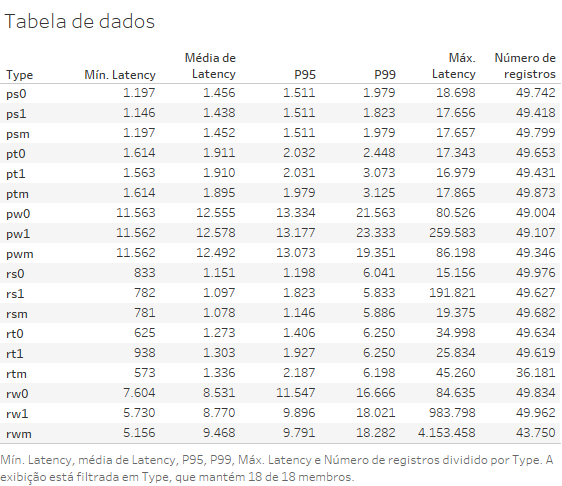
\includegraphics{graficos/Tabeladedados.png}
    \caption{Medições de latência}
    \label{tableau}
\end{figure}

\subsection{Comparativo por kernel}
\subsection{Comparativo por tipo de interrupção}
\subsection{Comparativo por carga de trabalho}
%\COM
 Resultados mais detalhados ser�o apresentados no cap�tulo
\ref{cap:implementacao}.
\MOC



\section{Estudou experimental)}
\label{cap:experimentos}

\section{Introdu��o}
\label{sec:introImp}

Nesta se��o, apresentar-se-� um estudo comparativo das quatro plataformas
apresentados no cap�tulo \ref{capSOTR}. Os experimentos realizados n�o tem
por objetivo de ser exaustivos. Eles apenas foram utilizados para entender
o comportamento temporal dos diferentes sistemas, tendo como foco principal
as lat�ncias de interrup��o e as lat�ncias de escalonamento relacionadas 
a camada de rede.

bla bla bla...


\section{Medidas de lat�ncias}
\label{sec:medLat}

Na se��o \ref{sec:latIRQ} do cap�tulo \ref{cap:SOTR}, o problema da medida das
lat�ncias de interrup��o foi brevemente apresentado. Uma das dificuldade apontada
foi esta da medi��o do instante exata no qual uma determinada interrup��o acontece
num certo hardware. Tendo como objetivo a compara��o das plataformas Linux, Linux
PREEMPT-RT, RTAI e Xenomai, adotou-se uma metodologia experimental simples,
inspirada de \cite{Proctor01}, que apesar de ser exclusivamente baseada em medidas
do rel�gio interno do computador, permitiu obter resultados significativos tanto quantitativa
quanto qualitativamente.

\subsection{O dispositivo experimental}
\label{sec:dispExp}

O dispositivo experimental utilizou a porta paralela, conectando um dos pinos
habilitados para escrita, presentemente o pino 9, ao pino 10 de interrup��o.  A
descri��o desta manipula��o e de v�rios exemplos de m�dulos para escrever na porta
paralela e capturar as interrup��es desta mesma porta foram encontrados no excelente
livro \ing{Linux Device Drivers} \cite{Corbet05}.  Para acessar valores de tempo
numa precis�o da ordem do $\mu s$, utilizou-se o contador do processador chamado de
\ing{Time Stamp Counter} (TSC)

Concretamente, um m�dulo especifico ($M$) foi desenvolvido para exportar as
funcionalidades seguintes:

\begin{itemize}
\item Acessar os 64 bits do TSC e gravar o valor na mem�ria.
\item Escrever na porta de entrada e sa�da 0x378 da porta paralela para gerar
  interrup��es de hardware.
\item Criar uma tarefa de tempo real $\tau$ que, possivelmente, executa algum c�digo
  �til. Neste experimento, $\tau$ simplesmente grava o valor do TSC.
\item Requisitar a captura das interrup��es na linha 7 associada a porta paralela e
  registrar o tratador de interrup��o $T_{pp}$ associado. $T_{pp}$ executa duas opera��es:
  (1) gravar o TSC; (2) Acordar $\tau$.
\item Implementar um canal de comunica��o FIFO ass�ncrono para transferir os dados
  coletados em modo protegido para o espa�o usu�rio.
\end{itemize}

Parte deste conjunto de fun��es foi disponibilizado sob forma de \cod{ioctl} para os processos
executando em modo usu�rio atrav�s de um arquivo especial \cod{/dev/M} do sistema de
arquivo. Outra parte � diretamente exportado sob forma de servi�os do \kernell
e podem ser acessadas somente por \ing{threads} do \kernell.

As medidas foram realizadas acompanhando o seguinte roteiro.  

\begin{itemize}
\item Ap�s a inser��o do m�dulo $M$ no \kernel, um processo $P$, executando em modo
  usu�rio, abre o arquivo especial \ing{/dev/M} para poder acessar as fun��es
  \ing{ioctl} disponibilizadas pelo m�dulo $M$. $P$ tenta ler o canal FIFO e fica
  bloqueado esperando dados.
\item Um computador remoto envia pacotes Ethernet numa freq��ncia de 20Hz para a
  esta��o de medi��o. No tratador de interrup��o $T-{eth}$ da placa de rede (RealTek
  8139), a fun��o de escrita na porta paralela � chamada.
\item No instante $t_1$ no qual $T$ executa a fun��o de escrita no pino 9 da
  porta paralela, o valor do TSC � memorizado na mem�ria do \kernel.
\item O tratador de interrup��o $T_{pp}$ da porta paralela � chamada. Ele grava o
  valor $t_2$ do TSC e acorda a tarefa $\tau$.
\item Eventualmente $\tau$ acorda e grava o valor $t_3$ do TSC e escreve o conjunto
  dos valores $t_1, t_2$ e $t_3$ no canal FIFO, antes de se suspender at� a pr�xima
  interrup��o na porta paralela.
\item $P$ � eventualmente acordado, e ap�s leitura do canal, escreve os dados num
  arquivo.
\end{itemize}

Este m�todo experimental tem as seguintes limita��es. Quando a interrup��o da placa
de rede acontece, o processador executa $T_{eth}$ no contexto do processo em
execu��o.  Depois de ter escrito na porta paralela, $T_{eth}$ retorna, e o
processador percebe imediatamente que uma outra interrup��o espere para ser
tratada. Ele portanto executa $T_{pp}$ em seguida, aproximadamente 10 $\mu s$
depois, possivelmente no contexto do mesmo processo que estava ocupando
o processador quando o pacote Ethernet chegou. Em 

 com uma troca de contexto m�nima.  
Por outro lado, este modo experimental garante que as interrup��es na porta
paralela sejam tratadas no contexto di
de gerar as interrup��es no contexto
da chegada de pacote Ethernet � que estes eventos s�o totalmente ass�ncronos em 
rela��o a atividade da esta��o de medi��o. 

No entanto, a principal vantagem 

Portanto, se o tempo de lat�ncia de
interrup��o observado � quase constante, 

Uma alternativa a este modo experimental � utilizar um processo para escrever
na porta paralela, mas neste caso, o processador sempre executaria $T_{pp}$ no
contexto deste processo. 
No entanto, este modo experimental foi preferido ao uso de um processo para escrever
na porta paralela por duas raz�es 

De fato, escrever no contexto da chegada de um pacote Ethernet 
tem a vantagem de ser  no lugar
do computador remot
antes de um
interrup��o, o processador est� sempre executando o processo usu�rio $P$ que acessa
a fun��o de \cod{ioctl} do m�dulo $M$ para escrever na porta paralela.  Portanto, a
presen�a de outros processos usu�rios sobrecarregando o processador n�o pode
interferir nas medidas. Uma outra limita��o provem do tempo de lat�ncia da pr�pria
porta paralela, que leva um certo tempo para estabilizar sua sa�da, na hora da
escrita. No entanto, os resultados obtidos usando esta metodologia podem servir para
medir um valor m�nimo do tempo de lat�ncia e para comparar diferentes plataformas
operacionais. Al�m disso, o impacto causado pela presen�a de outras atividades gerando
interrup��es pode ser observado. No caso deste trabalho, a placa de rede foi utilizado
para este efeito.

Observa que para evitar qualquer interfer�ncia nas medidas de lat�ncia, no caso do
Linux e de \preempt, o conjunto dos valores mensuradas foi salvo na mem�ria e
somente transferido para o sistema de arquivo depois do fim da execu��o do
experimento. Para as plataformas RTAI e Xenomai, foram utilizados os canais
\cod{RT-FIFO} de tempo real oferecidos pela API de ambas plataformas. A
implementa��o, sem \ing{lock}, destes canais garante a princ�pio a aus�ncia de
interfer�ncia com a execu��o das tarefas de tempo real no sistema.
 
No caso das duas plataformas RTAI e Xenomai, medidas complementares da lat�ncia de
escalonamento foram realizadas para avaliar a capacidade destas plataformas em
executar opera��es de transmiss�o de mensagens Ethernet com garantias
temporais. Para este efeito, o m�dulo $M$ foi acrescentado da seguinte maneira. Na
sua inser��o, ele cria uma tarefa $T$ (\ing{thread} de \kernel) que � acordada pelo
tratador de interrup��o da porta paralela. Quando a tarefa $T$ acorda, ela grava o
valor $t_3$ do TSC. Em seguida, $T$ executa a transmiss�o de um pacote Ethernet de
64 bytes, utilizando a fun��o \hardStartXmit, disponibilizada pelo controlador da
placa de rede.  No instante no qual esta fun��o � chamada, $T$ grava o valor $t_4$
do TSC. O valor da diferencia $t_3 - t_2$ representa portanto a lat�ncia de
escalonamento da tarefa $T$ e o valor $t_4 - t_3$, o tempo de execu��o necess�rio
para transmitir um pacote na rede.


\begin{sidewaysfigure}
  \centering
  \subfloat[Interrup��o - Sem estresse]{%
    \label{fig:kerSem}%
    {\scalebox{0.84}{\input{fig/kerSem}}}}
  \hspace{20pt}%
  \subfloat[][Escalonamento  - Sem estresse]{%
    \label{fig:kerSemSched}%
    {\scalebox{0.84}{\input{fig/kerSemSched}}}}\\%
%   \hspace{14pt}%
  \subfloat[Interrup��o - Com estresse]{%
    \label{fig:kerTot}%
    {\scalebox{0.84}{\input{fig/kerTot}}}}
  \hspace{20pt}%
  \subfloat[][Escalonamento  - Com estresse]{%
    \label{fig:kerTotSched}%
    {\scalebox{0.84}{\input{fig/kerTotSched}}}}%

  \caption[Lat�ncia de interrup��o e de escalonamento do Kernel Linux]{Lat�ncia de
    interrup��o e de escalonamento do Kernel Linux, vers�o 2.6.23.9, op��o
    \ing{Low-Latency}. As figuras \subref{fig:kerSem} e \subref{fig:kerSemSched}
    representam uma execu��o sem estresse e as figuras \subref{fig:kerTot} e
    \subref{fig:kerTotSched} representam uma execu��o com estresse do processador.
    A freq��ncia de escrita na porta paralela � de $20 Hz$.}
  \label{fig:klight}%
\end{sidewaysfigure}

\begin{sidewaysfigure}
  \centering
  \subfloat[Interrup��o - Sem estresse]{%
    \label{fig:preSem}%
    {\scalebox{0.84}{% GNUPLOT: LaTeX picture with Postscript
\begingroup
  \makeatletter
  \providecommand\color[2][]{%
    \GenericError{(gnuplot) \space\space\space\@spaces}{%
      Package color not loaded in conjunction with
      terminal option `colourtext'%
    }{See the gnuplot documentation for explanation.%
    }{Either use 'blacktext' in gnuplot or load the package
      color.sty in LaTeX.}%
    \renewcommand\color[2][]{}%
  }%
  \providecommand\includegraphics[2][]{%
    \GenericError{(gnuplot) \space\space\space\@spaces}{%
      Package graphicx or graphics not loaded%
    }{See the gnuplot documentation for explanation.%
    }{The gnuplot epslatex terminal needs graphicx.sty or graphics.sty.}%
    \renewcommand\includegraphics[2][]{}%
  }%
  \providecommand\rotatebox[2]{#2}%
  \@ifundefined{ifGPcolor}{%
    \newif\ifGPcolor
    \GPcolorfalse
  }{}%
  \@ifundefined{ifGPblacktext}{%
    \newif\ifGPblacktext
    \GPblacktextfalse
  }{}%
  % define a \g@addto@macro without @ in the name:
  \let\gplgaddtomacro\g@addto@macro
  % define empty templates for all commands taking text:
  \gdef\gplbacktext{}%
  \gdef\gplfronttext{}%
  \makeatother
  \ifGPblacktext
    % no textcolor at all
    \def\colorrgb#1{}%
    \def\colorgray#1{}%
  \else
    % gray or color?
    \ifGPcolor
      \def\colorrgb#1{\color[rgb]{#1}}%
      \def\colorgray#1{\color[gray]{#1}}%
      \expandafter\def\csname LTw\endcsname{\color{white}}%
      \expandafter\def\csname LTb\endcsname{\color{black}}%
      \expandafter\def\csname LTa\endcsname{\color{black}}%
      \expandafter\def\csname LT0\endcsname{\color[rgb]{1,0,0}}%
      \expandafter\def\csname LT1\endcsname{\color[rgb]{0,1,0}}%
      \expandafter\def\csname LT2\endcsname{\color[rgb]{0,0,1}}%
      \expandafter\def\csname LT3\endcsname{\color[rgb]{1,0,1}}%
      \expandafter\def\csname LT4\endcsname{\color[rgb]{0,1,1}}%
      \expandafter\def\csname LT5\endcsname{\color[rgb]{1,1,0}}%
      \expandafter\def\csname LT6\endcsname{\color[rgb]{0,0,0}}%
      \expandafter\def\csname LT7\endcsname{\color[rgb]{1,0.3,0}}%
      \expandafter\def\csname LT8\endcsname{\color[rgb]{0.5,0.5,0.5}}%
    \else
      % gray
      \def\colorrgb#1{\color{black}}%
      \def\colorgray#1{\color[gray]{#1}}%
      \expandafter\def\csname LTw\endcsname{\color{white}}%
      \expandafter\def\csname LTb\endcsname{\color{black}}%
      \expandafter\def\csname LTa\endcsname{\color{black}}%
      \expandafter\def\csname LT0\endcsname{\color{black}}%
      \expandafter\def\csname LT1\endcsname{\color{black}}%
      \expandafter\def\csname LT2\endcsname{\color{black}}%
      \expandafter\def\csname LT3\endcsname{\color{black}}%
      \expandafter\def\csname LT4\endcsname{\color{black}}%
      \expandafter\def\csname LT5\endcsname{\color{black}}%
      \expandafter\def\csname LT6\endcsname{\color{black}}%
      \expandafter\def\csname LT7\endcsname{\color{black}}%
      \expandafter\def\csname LT8\endcsname{\color{black}}%
    \fi
  \fi
  \setlength{\unitlength}{0.0500bp}%
  \begin{picture}(7200.00,5040.00)%
    \gplgaddtomacro\gplbacktext{%
      \csname LTb\endcsname%
      \put(1034,873){\makebox(0,0)[r]{\strut{}$16.0$}}%
      \put(1034,1430){\makebox(0,0)[r]{\strut{}$18.0$}}%
      \put(1034,1988){\makebox(0,0)[r]{\strut{}$20.0$}}%
      \put(1034,2546){\makebox(0,0)[r]{\strut{}$22.0$}}%
      \put(1034,3103){\makebox(0,0)[r]{\strut{}$24.0$}}%
      \put(1034,3661){\makebox(0,0)[r]{\strut{}$26.0$}}%
      \put(1034,4218){\makebox(0,0)[r]{\strut{}$28.0$}}%
      \put(1034,4776){\makebox(0,0)[r]{\strut{}$30.0$}}%
      \put(1166,374){\makebox(0,0){\strut{}$ 0$}}%
      \put(2109,374){\makebox(0,0){\strut{}$ 10$}}%
      \put(3053,374){\makebox(0,0){\strut{}$ 20$}}%
      \put(3996,374){\makebox(0,0){\strut{}$ 30$}}%
      \put(4939,374){\makebox(0,0){\strut{}$ 40$}}%
      \put(5883,374){\makebox(0,0){\strut{}$ 50$}}%
      \put(6826,374){\makebox(0,0){\strut{}$ 60$}}%
      \put(396,2685){\rotatebox{90}{\makebox(0,0){\strut{}Lat\^encia em $\mu s$}}}%
      \put(3996,110){\makebox(0,0){\strut{}Tempo de observa\c{c}\~ao em $s$}}%
    }%
    \gplgaddtomacro\gplfronttext{%
    }%
    \gplbacktext
    \put(0,0){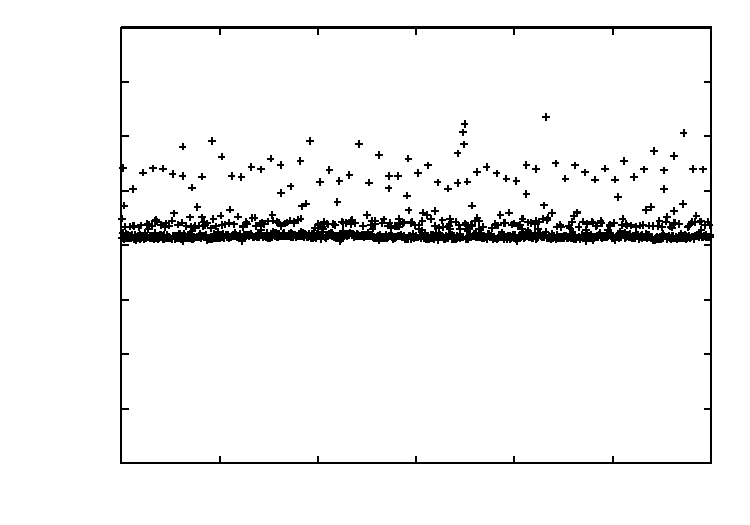
\includegraphics{fig2/preSem}}%
    \gplfronttext
  \end{picture}%
\endgroup
}}}
  \hspace{20pt}%
  \subfloat[][Escalonamento  - Sem estresse]{%
    \label{fig:preSemSched}%
    {\scalebox{0.84}{% GNUPLOT: LaTeX picture with Postscript
\begingroup
  \makeatletter
  \providecommand\color[2][]{%
    \GenericError{(gnuplot) \space\space\space\@spaces}{%
      Package color not loaded in conjunction with
      terminal option `colourtext'%
    }{See the gnuplot documentation for explanation.%
    }{Either use 'blacktext' in gnuplot or load the package
      color.sty in LaTeX.}%
    \renewcommand\color[2][]{}%
  }%
  \providecommand\includegraphics[2][]{%
    \GenericError{(gnuplot) \space\space\space\@spaces}{%
      Package graphicx or graphics not loaded%
    }{See the gnuplot documentation for explanation.%
    }{The gnuplot epslatex terminal needs graphicx.sty or graphics.sty.}%
    \renewcommand\includegraphics[2][]{}%
  }%
  \providecommand\rotatebox[2]{#2}%
  \@ifundefined{ifGPcolor}{%
    \newif\ifGPcolor
    \GPcolorfalse
  }{}%
  \@ifundefined{ifGPblacktext}{%
    \newif\ifGPblacktext
    \GPblacktextfalse
  }{}%
  % define a \g@addto@macro without @ in the name:
  \let\gplgaddtomacro\g@addto@macro
  % define empty templates for all commands taking text:
  \gdef\gplbacktext{}%
  \gdef\gplfronttext{}%
  \makeatother
  \ifGPblacktext
    % no textcolor at all
    \def\colorrgb#1{}%
    \def\colorgray#1{}%
  \else
    % gray or color?
    \ifGPcolor
      \def\colorrgb#1{\color[rgb]{#1}}%
      \def\colorgray#1{\color[gray]{#1}}%
      \expandafter\def\csname LTw\endcsname{\color{white}}%
      \expandafter\def\csname LTb\endcsname{\color{black}}%
      \expandafter\def\csname LTa\endcsname{\color{black}}%
      \expandafter\def\csname LT0\endcsname{\color[rgb]{1,0,0}}%
      \expandafter\def\csname LT1\endcsname{\color[rgb]{0,1,0}}%
      \expandafter\def\csname LT2\endcsname{\color[rgb]{0,0,1}}%
      \expandafter\def\csname LT3\endcsname{\color[rgb]{1,0,1}}%
      \expandafter\def\csname LT4\endcsname{\color[rgb]{0,1,1}}%
      \expandafter\def\csname LT5\endcsname{\color[rgb]{1,1,0}}%
      \expandafter\def\csname LT6\endcsname{\color[rgb]{0,0,0}}%
      \expandafter\def\csname LT7\endcsname{\color[rgb]{1,0.3,0}}%
      \expandafter\def\csname LT8\endcsname{\color[rgb]{0.5,0.5,0.5}}%
    \else
      % gray
      \def\colorrgb#1{\color{black}}%
      \def\colorgray#1{\color[gray]{#1}}%
      \expandafter\def\csname LTw\endcsname{\color{white}}%
      \expandafter\def\csname LTb\endcsname{\color{black}}%
      \expandafter\def\csname LTa\endcsname{\color{black}}%
      \expandafter\def\csname LT0\endcsname{\color{black}}%
      \expandafter\def\csname LT1\endcsname{\color{black}}%
      \expandafter\def\csname LT2\endcsname{\color{black}}%
      \expandafter\def\csname LT3\endcsname{\color{black}}%
      \expandafter\def\csname LT4\endcsname{\color{black}}%
      \expandafter\def\csname LT5\endcsname{\color{black}}%
      \expandafter\def\csname LT6\endcsname{\color{black}}%
      \expandafter\def\csname LT7\endcsname{\color{black}}%
      \expandafter\def\csname LT8\endcsname{\color{black}}%
    \fi
  \fi
  \setlength{\unitlength}{0.0500bp}%
  \begin{picture}(7200.00,5040.00)%
    \gplgaddtomacro\gplbacktext{%
      \csname LTb\endcsname%
      \put(1034,594){\makebox(0,0)[r]{\strut{}$0.0$}}%
      \put(1034,1640){\makebox(0,0)[r]{\strut{}$5.0$}}%
      \put(1034,2685){\makebox(0,0)[r]{\strut{}$10.0$}}%
      \put(1034,3731){\makebox(0,0)[r]{\strut{}$15.0$}}%
      \put(1034,4776){\makebox(0,0)[r]{\strut{}$20.0$}}%
      \put(1166,374){\makebox(0,0){\strut{}$ 0$}}%
      \put(2109,374){\makebox(0,0){\strut{}$ 10$}}%
      \put(3053,374){\makebox(0,0){\strut{}$ 20$}}%
      \put(3996,374){\makebox(0,0){\strut{}$ 30$}}%
      \put(4939,374){\makebox(0,0){\strut{}$ 40$}}%
      \put(5883,374){\makebox(0,0){\strut{}$ 50$}}%
      \put(6826,374){\makebox(0,0){\strut{}$ 60$}}%
      \put(396,2685){\rotatebox{90}{\makebox(0,0){\strut{}Lat\^encia em $\mu s$}}}%
      \put(3996,110){\makebox(0,0){\strut{}Tempo de observa\c{c}\~ao em $s$}}%
    }%
    \gplgaddtomacro\gplfronttext{%
    }%
    \gplbacktext
    \put(0,0){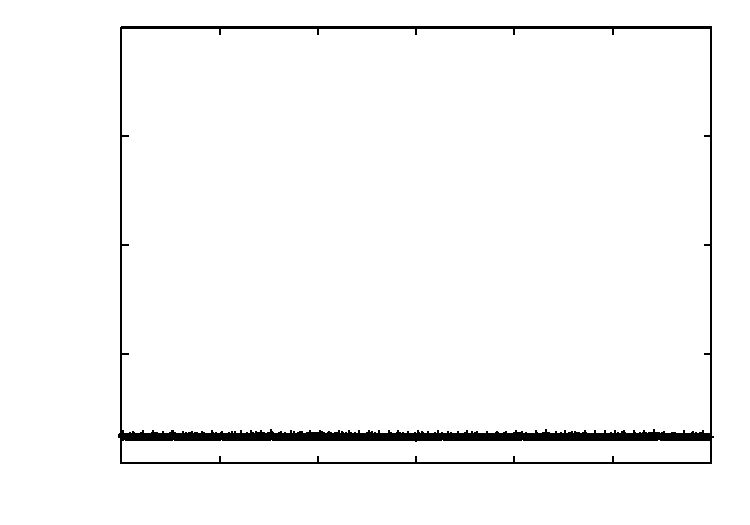
\includegraphics{fig/preSemSched.pdf}}%
    \gplfronttext
  \end{picture}%
\endgroup
}}}\\%
%   \hspace{14pt}%
  \subfloat[Interrup��o - Com estresse]{%
    \label{fig:preTot}%
    {\scalebox{0.84}{% GNUPLOT: LaTeX picture with Postscript
\begingroup
  \makeatletter
  \providecommand\color[2][]{%
    \GenericError{(gnuplot) \space\space\space\@spaces}{%
      Package color not loaded in conjunction with
      terminal option `colourtext'%
    }{See the gnuplot documentation for explanation.%
    }{Either use 'blacktext' in gnuplot or load the package
      color.sty in LaTeX.}%
    \renewcommand\color[2][]{}%
  }%
  \providecommand\includegraphics[2][]{%
    \GenericError{(gnuplot) \space\space\space\@spaces}{%
      Package graphicx or graphics not loaded%
    }{See the gnuplot documentation for explanation.%
    }{The gnuplot epslatex terminal needs graphicx.sty or graphics.sty.}%
    \renewcommand\includegraphics[2][]{}%
  }%
  \providecommand\rotatebox[2]{#2}%
  \@ifundefined{ifGPcolor}{%
    \newif\ifGPcolor
    \GPcolorfalse
  }{}%
  \@ifundefined{ifGPblacktext}{%
    \newif\ifGPblacktext
    \GPblacktextfalse
  }{}%
  % define a \g@addto@macro without @ in the name:
  \let\gplgaddtomacro\g@addto@macro
  % define empty templates for all commands taking text:
  \gdef\gplbacktext{}%
  \gdef\gplfronttext{}%
  \makeatother
  \ifGPblacktext
    % no textcolor at all
    \def\colorrgb#1{}%
    \def\colorgray#1{}%
  \else
    % gray or color?
    \ifGPcolor
      \def\colorrgb#1{\color[rgb]{#1}}%
      \def\colorgray#1{\color[gray]{#1}}%
      \expandafter\def\csname LTw\endcsname{\color{white}}%
      \expandafter\def\csname LTb\endcsname{\color{black}}%
      \expandafter\def\csname LTa\endcsname{\color{black}}%
      \expandafter\def\csname LT0\endcsname{\color[rgb]{1,0,0}}%
      \expandafter\def\csname LT1\endcsname{\color[rgb]{0,1,0}}%
      \expandafter\def\csname LT2\endcsname{\color[rgb]{0,0,1}}%
      \expandafter\def\csname LT3\endcsname{\color[rgb]{1,0,1}}%
      \expandafter\def\csname LT4\endcsname{\color[rgb]{0,1,1}}%
      \expandafter\def\csname LT5\endcsname{\color[rgb]{1,1,0}}%
      \expandafter\def\csname LT6\endcsname{\color[rgb]{0,0,0}}%
      \expandafter\def\csname LT7\endcsname{\color[rgb]{1,0.3,0}}%
      \expandafter\def\csname LT8\endcsname{\color[rgb]{0.5,0.5,0.5}}%
    \else
      % gray
      \def\colorrgb#1{\color{black}}%
      \def\colorgray#1{\color[gray]{#1}}%
      \expandafter\def\csname LTw\endcsname{\color{white}}%
      \expandafter\def\csname LTb\endcsname{\color{black}}%
      \expandafter\def\csname LTa\endcsname{\color{black}}%
      \expandafter\def\csname LT0\endcsname{\color{black}}%
      \expandafter\def\csname LT1\endcsname{\color{black}}%
      \expandafter\def\csname LT2\endcsname{\color{black}}%
      \expandafter\def\csname LT3\endcsname{\color{black}}%
      \expandafter\def\csname LT4\endcsname{\color{black}}%
      \expandafter\def\csname LT5\endcsname{\color{black}}%
      \expandafter\def\csname LT6\endcsname{\color{black}}%
      \expandafter\def\csname LT7\endcsname{\color{black}}%
      \expandafter\def\csname LT8\endcsname{\color{black}}%
    \fi
  \fi
  \setlength{\unitlength}{0.0500bp}%
  \begin{picture}(7200.00,5040.00)%
    \gplgaddtomacro\gplbacktext{%
      \csname LTb\endcsname%
      \put(1034,594){\makebox(0,0)[r]{\strut{}$0.0$}}%
      \put(1034,1430){\makebox(0,0)[r]{\strut{}$10.0$}}%
      \put(1034,2267){\makebox(0,0)[r]{\strut{}$20.0$}}%
      \put(1034,3103){\makebox(0,0)[r]{\strut{}$30.0$}}%
      \put(1034,3940){\makebox(0,0)[r]{\strut{}$40.0$}}%
      \put(1034,4776){\makebox(0,0)[r]{\strut{}$50.0$}}%
      \put(1166,374){\makebox(0,0){\strut{}$ 0$}}%
      \put(2109,374){\makebox(0,0){\strut{}$ 10$}}%
      \put(3053,374){\makebox(0,0){\strut{}$ 20$}}%
      \put(3996,374){\makebox(0,0){\strut{}$ 30$}}%
      \put(4939,374){\makebox(0,0){\strut{}$ 40$}}%
      \put(5883,374){\makebox(0,0){\strut{}$ 50$}}%
      \put(6826,374){\makebox(0,0){\strut{}$ 60$}}%
      \put(396,2685){\rotatebox{90}{\makebox(0,0){\strut{}Latency ($\mu s$)}}}%
      \put(3996,110){\makebox(0,0){\strut{}Time ($s$)}}%
    }%
    \gplgaddtomacro\gplfronttext{%
    }%
    \gplbacktext
    \put(0,0){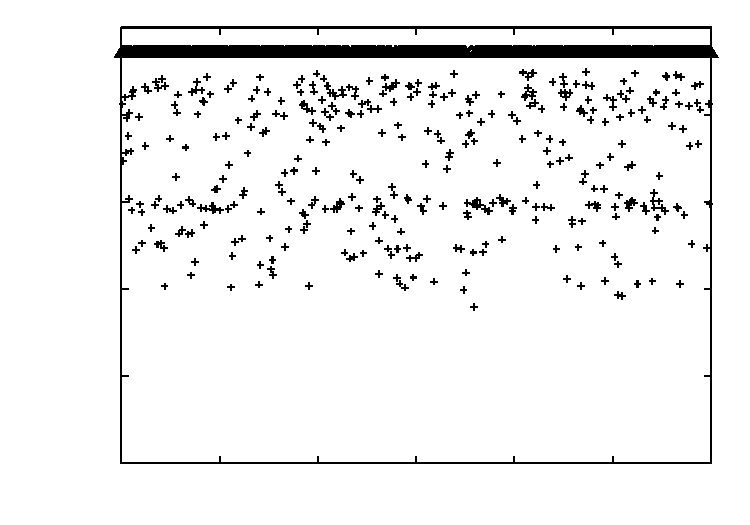
\includegraphics{fig/preTot.pdf}}%
    \gplfronttext
  \end{picture}%
\endgroup
}}}
  \hspace{20pt}%
  \subfloat[][Escalonamento  - Com estresse]{%
    \label{fig:preTotSched}%
    {\scalebox{0.84}{% GNUPLOT: LaTeX picture with Postscript
\begingroup
  \makeatletter
  \providecommand\color[2][]{%
    \GenericError{(gnuplot) \space\space\space\@spaces}{%
      Package color not loaded in conjunction with
      terminal option `colourtext'%
    }{See the gnuplot documentation for explanation.%
    }{Either use 'blacktext' in gnuplot or load the package
      color.sty in LaTeX.}%
    \renewcommand\color[2][]{}%
  }%
  \providecommand\includegraphics[2][]{%
    \GenericError{(gnuplot) \space\space\space\@spaces}{%
      Package graphicx or graphics not loaded%
    }{See the gnuplot documentation for explanation.%
    }{The gnuplot epslatex terminal needs graphicx.sty or graphics.sty.}%
    \renewcommand\includegraphics[2][]{}%
  }%
  \providecommand\rotatebox[2]{#2}%
  \@ifundefined{ifGPcolor}{%
    \newif\ifGPcolor
    \GPcolorfalse
  }{}%
  \@ifundefined{ifGPblacktext}{%
    \newif\ifGPblacktext
    \GPblacktextfalse
  }{}%
  % define a \g@addto@macro without @ in the name:
  \let\gplgaddtomacro\g@addto@macro
  % define empty templates for all commands taking text:
  \gdef\gplbacktext{}%
  \gdef\gplfronttext{}%
  \makeatother
  \ifGPblacktext
    % no textcolor at all
    \def\colorrgb#1{}%
    \def\colorgray#1{}%
  \else
    % gray or color?
    \ifGPcolor
      \def\colorrgb#1{\color[rgb]{#1}}%
      \def\colorgray#1{\color[gray]{#1}}%
      \expandafter\def\csname LTw\endcsname{\color{white}}%
      \expandafter\def\csname LTb\endcsname{\color{black}}%
      \expandafter\def\csname LTa\endcsname{\color{black}}%
      \expandafter\def\csname LT0\endcsname{\color[rgb]{1,0,0}}%
      \expandafter\def\csname LT1\endcsname{\color[rgb]{0,1,0}}%
      \expandafter\def\csname LT2\endcsname{\color[rgb]{0,0,1}}%
      \expandafter\def\csname LT3\endcsname{\color[rgb]{1,0,1}}%
      \expandafter\def\csname LT4\endcsname{\color[rgb]{0,1,1}}%
      \expandafter\def\csname LT5\endcsname{\color[rgb]{1,1,0}}%
      \expandafter\def\csname LT6\endcsname{\color[rgb]{0,0,0}}%
      \expandafter\def\csname LT7\endcsname{\color[rgb]{1,0.3,0}}%
      \expandafter\def\csname LT8\endcsname{\color[rgb]{0.5,0.5,0.5}}%
    \else
      % gray
      \def\colorrgb#1{\color{black}}%
      \def\colorgray#1{\color[gray]{#1}}%
      \expandafter\def\csname LTw\endcsname{\color{white}}%
      \expandafter\def\csname LTb\endcsname{\color{black}}%
      \expandafter\def\csname LTa\endcsname{\color{black}}%
      \expandafter\def\csname LT0\endcsname{\color{black}}%
      \expandafter\def\csname LT1\endcsname{\color{black}}%
      \expandafter\def\csname LT2\endcsname{\color{black}}%
      \expandafter\def\csname LT3\endcsname{\color{black}}%
      \expandafter\def\csname LT4\endcsname{\color{black}}%
      \expandafter\def\csname LT5\endcsname{\color{black}}%
      \expandafter\def\csname LT6\endcsname{\color{black}}%
      \expandafter\def\csname LT7\endcsname{\color{black}}%
      \expandafter\def\csname LT8\endcsname{\color{black}}%
    \fi
  \fi
  \setlength{\unitlength}{0.0500bp}%
  \begin{picture}(7200.00,5040.00)%
    \gplgaddtomacro\gplbacktext{%
      \csname LTb\endcsname%
      \put(1034,594){\makebox(0,0)[r]{\strut{}$0.0$}}%
      \put(1034,1640){\makebox(0,0)[r]{\strut{}$5.0$}}%
      \put(1034,2685){\makebox(0,0)[r]{\strut{}$10.0$}}%
      \put(1034,3731){\makebox(0,0)[r]{\strut{}$15.0$}}%
      \put(1034,4776){\makebox(0,0)[r]{\strut{}$20.0$}}%
      \put(1166,374){\makebox(0,0){\strut{}$ 0$}}%
      \put(2109,374){\makebox(0,0){\strut{}$ 10$}}%
      \put(3053,374){\makebox(0,0){\strut{}$ 20$}}%
      \put(3996,374){\makebox(0,0){\strut{}$ 30$}}%
      \put(4939,374){\makebox(0,0){\strut{}$ 40$}}%
      \put(5883,374){\makebox(0,0){\strut{}$ 50$}}%
      \put(6826,374){\makebox(0,0){\strut{}$ 60$}}%
      \put(396,2685){\rotatebox{90}{\makebox(0,0){\strut{}Lat\^encia em $\mu s$}}}%
      \put(3996,110){\makebox(0,0){\strut{}Tempo de observa\c{c}\~ao em $s$}}%
    }%
    \gplgaddtomacro\gplfronttext{%
    }%
    \gplbacktext
    \put(0,0){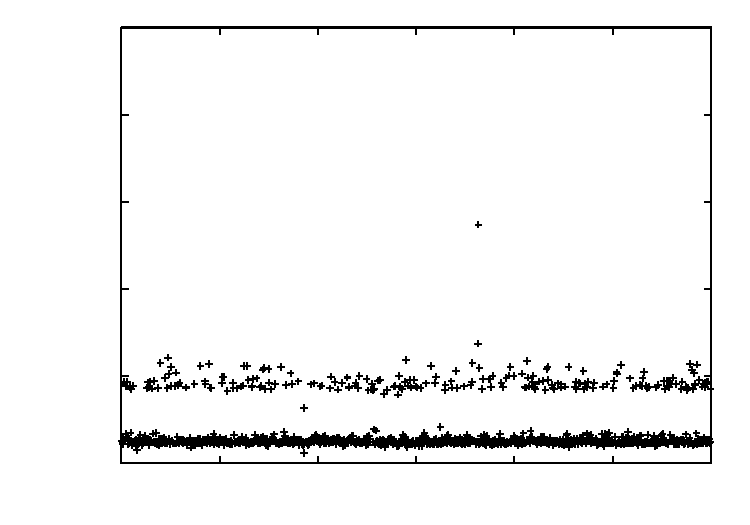
\includegraphics{fig/preTotSched}}%
    \gplfronttext
  \end{picture}%
\endgroup
}}}%

  \caption[Lat�ncia de interrup��o e de escalonamento de PREEMPT-RT]{Lat�ncia de
    interrup��o e de escalonamento do \ing{patch} PREEMPT-RT instalado no \kernel
    Linux, vers�o 2.6.23.9. As figuras \subref{fig:preSem} e
    \subref{fig:preSemSched} representam uma execu��o sem estresse e as figuras
    \subref{fig:preTot} e \subref{fig:preTotSched} representam uma execu��o com
    estresse do processador.  A freq��ncia de escrita na porta paralela � de $20
    Hz$.}
  \label{fig:preemptExp}%
\end{sidewaysfigure}

\begin{sidewaysfigure}
  \centering
  \subfloat[Interrup��o - Sem estresse]{%
    \label{fig:xenSem}%
    {\scalebox{0.84}{% GNUPLOT: LaTeX picture with Postscript
\begingroup
  \makeatletter
  \providecommand\color[2][]{%
    \GenericError{(gnuplot) \space\space\space\@spaces}{%
      Package color not loaded in conjunction with
      terminal option `colourtext'%
    }{See the gnuplot documentation for explanation.%
    }{Either use 'blacktext' in gnuplot or load the package
      color.sty in LaTeX.}%
    \renewcommand\color[2][]{}%
  }%
  \providecommand\includegraphics[2][]{%
    \GenericError{(gnuplot) \space\space\space\@spaces}{%
      Package graphicx or graphics not loaded%
    }{See the gnuplot documentation for explanation.%
    }{The gnuplot epslatex terminal needs graphicx.sty or graphics.sty.}%
    \renewcommand\includegraphics[2][]{}%
  }%
  \providecommand\rotatebox[2]{#2}%
  \@ifundefined{ifGPcolor}{%
    \newif\ifGPcolor
    \GPcolorfalse
  }{}%
  \@ifundefined{ifGPblacktext}{%
    \newif\ifGPblacktext
    \GPblacktexttrue
  }{}%
  % define a \g@addto@macro without @ in the name:
  \let\gplgaddtomacro\g@addto@macro
  % define empty templates for all commands taking text:
  \gdef\gplbacktext{}%
  \gdef\gplfronttext{}%
  \makeatother
  \ifGPblacktext
    % no textcolor at all
    \def\colorrgb#1{}%
    \def\colorgray#1{}%
  \else
    % gray or color?
    \ifGPcolor
      \def\colorrgb#1{\color[rgb]{#1}}%
      \def\colorgray#1{\color[gray]{#1}}%
      \expandafter\def\csname LTw\endcsname{\color{white}}%
      \expandafter\def\csname LTb\endcsname{\color{black}}%
      \expandafter\def\csname LTa\endcsname{\color{black}}%
      \expandafter\def\csname LT0\endcsname{\color[rgb]{1,0,0}}%
      \expandafter\def\csname LT1\endcsname{\color[rgb]{0,1,0}}%
      \expandafter\def\csname LT2\endcsname{\color[rgb]{0,0,1}}%
      \expandafter\def\csname LT3\endcsname{\color[rgb]{1,0,1}}%
      \expandafter\def\csname LT4\endcsname{\color[rgb]{0,1,1}}%
      \expandafter\def\csname LT5\endcsname{\color[rgb]{1,1,0}}%
      \expandafter\def\csname LT6\endcsname{\color[rgb]{0,0,0}}%
      \expandafter\def\csname LT7\endcsname{\color[rgb]{1,0.3,0}}%
      \expandafter\def\csname LT8\endcsname{\color[rgb]{0.5,0.5,0.5}}%
    \else
      % gray
      \def\colorrgb#1{\color{black}}%
      \def\colorgray#1{\color[gray]{#1}}%
      \expandafter\def\csname LTw\endcsname{\color{white}}%
      \expandafter\def\csname LTb\endcsname{\color{black}}%
      \expandafter\def\csname LTa\endcsname{\color{black}}%
      \expandafter\def\csname LT0\endcsname{\color{black}}%
      \expandafter\def\csname LT1\endcsname{\color{black}}%
      \expandafter\def\csname LT2\endcsname{\color{black}}%
      \expandafter\def\csname LT3\endcsname{\color{black}}%
      \expandafter\def\csname LT4\endcsname{\color{black}}%
      \expandafter\def\csname LT5\endcsname{\color{black}}%
      \expandafter\def\csname LT6\endcsname{\color{black}}%
      \expandafter\def\csname LT7\endcsname{\color{black}}%
      \expandafter\def\csname LT8\endcsname{\color{black}}%
    \fi
  \fi
  \setlength{\unitlength}{0.0500bp}%
  \begin{picture}(7200.00,5040.00)%
    \gplgaddtomacro\gplbacktext{%
      \csname LTb\endcsname%
      \put(1386,660){\makebox(0,0)[r]{\strut{}$0.0$}}%
      \put(1386,1483){\makebox(0,0)[r]{\strut{}$20.0$}}%
      \put(1386,2306){\makebox(0,0)[r]{\strut{}$40.0$}}%
      \put(1386,3130){\makebox(0,0)[r]{\strut{}$60.0$}}%
      \put(1386,3953){\makebox(0,0)[r]{\strut{}$80.0$}}%
      \put(1386,4776){\makebox(0,0)[r]{\strut{}$100.0$}}%
      \put(1518,440){\makebox(0,0){\strut{}$ 0$}}%
      \put(2403,440){\makebox(0,0){\strut{}$ 10$}}%
      \put(3287,440){\makebox(0,0){\strut{}$ 20$}}%
      \put(4172,440){\makebox(0,0){\strut{}$ 30$}}%
      \put(5057,440){\makebox(0,0){\strut{}$ 40$}}%
      \put(5941,440){\makebox(0,0){\strut{}$ 50$}}%
      \put(6826,440){\makebox(0,0){\strut{}$ 60$}}%
      \put(220,2718){\rotatebox{90}{\makebox(0,0){\strut{}Lat\^encia em $\mu s$}}}%
      \put(4172,110){\makebox(0,0){\strut{}Tempo de observa\c{c}\~ao em $s$}}%
    }%
    \gplgaddtomacro\gplfronttext{%
    }%
    \gplbacktext
    \put(0,0){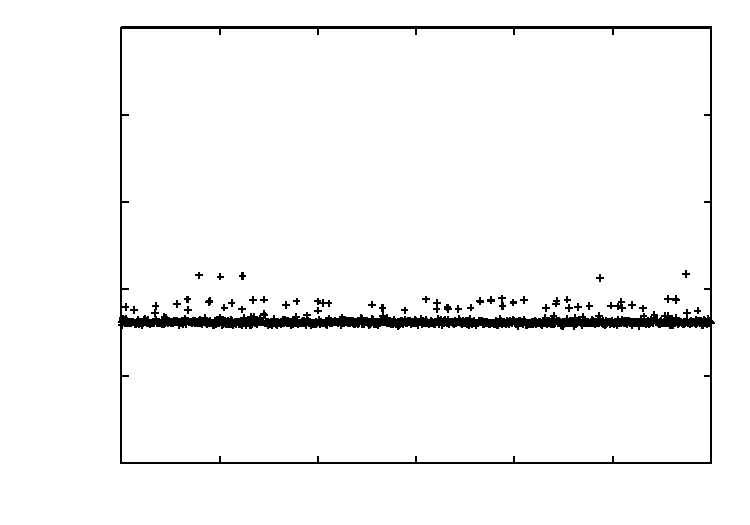
\includegraphics{fig/xenSem}}%
    \gplfronttext
  \end{picture}%
\endgroup
}}}
  \hspace{20pt}%
  \subfloat[][Escalonamento  - Sem estresse]{%
    \label{fig:xenSemSched}%
    {\scalebox{0.84}{% GNUPLOT: LaTeX picture with Postscript
\begingroup
  \makeatletter
  \providecommand\color[2][]{%
    \GenericError{(gnuplot) \space\space\space\@spaces}{%
      Package color not loaded in conjunction with
      terminal option `colourtext'%
    }{See the gnuplot documentation for explanation.%
    }{Either use 'blacktext' in gnuplot or load the package
      color.sty in LaTeX.}%
    \renewcommand\color[2][]{}%
  }%
  \providecommand\includegraphics[2][]{%
    \GenericError{(gnuplot) \space\space\space\@spaces}{%
      Package graphicx or graphics not loaded%
    }{See the gnuplot documentation for explanation.%
    }{The gnuplot epslatex terminal needs graphicx.sty or graphics.sty.}%
    \renewcommand\includegraphics[2][]{}%
  }%
  \providecommand\rotatebox[2]{#2}%
  \@ifundefined{ifGPcolor}{%
    \newif\ifGPcolor
    \GPcolorfalse
  }{}%
  \@ifundefined{ifGPblacktext}{%
    \newif\ifGPblacktext
    \GPblacktextfalse
  }{}%
  % define a \g@addto@macro without @ in the name:
  \let\gplgaddtomacro\g@addto@macro
  % define empty templates for all commands taking text:
  \gdef\gplbacktext{}%
  \gdef\gplfronttext{}%
  \makeatother
  \ifGPblacktext
    % no textcolor at all
    \def\colorrgb#1{}%
    \def\colorgray#1{}%
  \else
    % gray or color?
    \ifGPcolor
      \def\colorrgb#1{\color[rgb]{#1}}%
      \def\colorgray#1{\color[gray]{#1}}%
      \expandafter\def\csname LTw\endcsname{\color{white}}%
      \expandafter\def\csname LTb\endcsname{\color{black}}%
      \expandafter\def\csname LTa\endcsname{\color{black}}%
      \expandafter\def\csname LT0\endcsname{\color[rgb]{1,0,0}}%
      \expandafter\def\csname LT1\endcsname{\color[rgb]{0,1,0}}%
      \expandafter\def\csname LT2\endcsname{\color[rgb]{0,0,1}}%
      \expandafter\def\csname LT3\endcsname{\color[rgb]{1,0,1}}%
      \expandafter\def\csname LT4\endcsname{\color[rgb]{0,1,1}}%
      \expandafter\def\csname LT5\endcsname{\color[rgb]{1,1,0}}%
      \expandafter\def\csname LT6\endcsname{\color[rgb]{0,0,0}}%
      \expandafter\def\csname LT7\endcsname{\color[rgb]{1,0.3,0}}%
      \expandafter\def\csname LT8\endcsname{\color[rgb]{0.5,0.5,0.5}}%
    \else
      % gray
      \def\colorrgb#1{\color{black}}%
      \def\colorgray#1{\color[gray]{#1}}%
      \expandafter\def\csname LTw\endcsname{\color{white}}%
      \expandafter\def\csname LTb\endcsname{\color{black}}%
      \expandafter\def\csname LTa\endcsname{\color{black}}%
      \expandafter\def\csname LT0\endcsname{\color{black}}%
      \expandafter\def\csname LT1\endcsname{\color{black}}%
      \expandafter\def\csname LT2\endcsname{\color{black}}%
      \expandafter\def\csname LT3\endcsname{\color{black}}%
      \expandafter\def\csname LT4\endcsname{\color{black}}%
      \expandafter\def\csname LT5\endcsname{\color{black}}%
      \expandafter\def\csname LT6\endcsname{\color{black}}%
      \expandafter\def\csname LT7\endcsname{\color{black}}%
      \expandafter\def\csname LT8\endcsname{\color{black}}%
    \fi
  \fi
  \setlength{\unitlength}{0.0500bp}%
  \begin{picture}(7200.00,5040.00)%
    \gplgaddtomacro\gplbacktext{%
      \csname LTb\endcsname%
      \put(1034,594){\makebox(0,0)[r]{\strut{}$0.0$}}%
      \put(1034,1640){\makebox(0,0)[r]{\strut{}$5.0$}}%
      \put(1034,2685){\makebox(0,0)[r]{\strut{}$10.0$}}%
      \put(1034,3731){\makebox(0,0)[r]{\strut{}$15.0$}}%
      \put(1034,4776){\makebox(0,0)[r]{\strut{}$20.0$}}%
      \put(1166,374){\makebox(0,0){\strut{}$ 0$}}%
      \put(2109,374){\makebox(0,0){\strut{}$ 10$}}%
      \put(3053,374){\makebox(0,0){\strut{}$ 20$}}%
      \put(3996,374){\makebox(0,0){\strut{}$ 30$}}%
      \put(4939,374){\makebox(0,0){\strut{}$ 40$}}%
      \put(5883,374){\makebox(0,0){\strut{}$ 50$}}%
      \put(6826,374){\makebox(0,0){\strut{}$ 60$}}%
      \put(396,2685){\rotatebox{90}{\makebox(0,0){\strut{}Lat\^encia em $\mu s$}}}%
      \put(3996,110){\makebox(0,0){\strut{}Tempo de observa\c{c}\~ao em $s$}}%
    }%
    \gplgaddtomacro\gplfronttext{%
    }%
    \gplbacktext
    \put(0,0){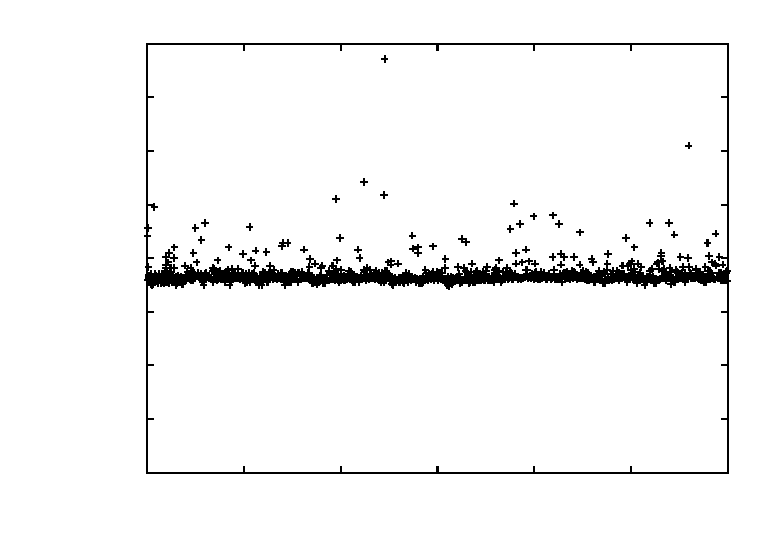
\includegraphics{fig/xenSemSched}}%
    \gplfronttext
  \end{picture}%
\endgroup
}}}\\%
%   \hspace{14pt}%
  \subfloat[Interrup��o - Com estresse]{%
    \label{fig:xenTot}%
    {\scalebox{0.84}{% GNUPLOT: LaTeX picture with Postscript
\begingroup
  \makeatletter
  \providecommand\color[2][]{%
    \GenericError{(gnuplot) \space\space\space\@spaces}{%
      Package color not loaded in conjunction with
      terminal option `colourtext'%
    }{See the gnuplot documentation for explanation.%
    }{Either use 'blacktext' in gnuplot or load the package
      color.sty in LaTeX.}%
    \renewcommand\color[2][]{}%
  }%
  \providecommand\includegraphics[2][]{%
    \GenericError{(gnuplot) \space\space\space\@spaces}{%
      Package graphicx or graphics not loaded%
    }{See the gnuplot documentation for explanation.%
    }{The gnuplot epslatex terminal needs graphicx.sty or graphics.sty.}%
    \renewcommand\includegraphics[2][]{}%
  }%
  \providecommand\rotatebox[2]{#2}%
  \@ifundefined{ifGPcolor}{%
    \newif\ifGPcolor
    \GPcolorfalse
  }{}%
  \@ifundefined{ifGPblacktext}{%
    \newif\ifGPblacktext
    \GPblacktextfalse
  }{}%
  % define a \g@addto@macro without @ in the name:
  \let\gplgaddtomacro\g@addto@macro
  % define empty templates for all commands taking text:
  \gdef\gplbacktext{}%
  \gdef\gplfronttext{}%
  \makeatother
  \ifGPblacktext
    % no textcolor at all
    \def\colorrgb#1{}%
    \def\colorgray#1{}%
  \else
    % gray or color?
    \ifGPcolor
      \def\colorrgb#1{\color[rgb]{#1}}%
      \def\colorgray#1{\color[gray]{#1}}%
      \expandafter\def\csname LTw\endcsname{\color{white}}%
      \expandafter\def\csname LTb\endcsname{\color{black}}%
      \expandafter\def\csname LTa\endcsname{\color{black}}%
      \expandafter\def\csname LT0\endcsname{\color[rgb]{1,0,0}}%
      \expandafter\def\csname LT1\endcsname{\color[rgb]{0,1,0}}%
      \expandafter\def\csname LT2\endcsname{\color[rgb]{0,0,1}}%
      \expandafter\def\csname LT3\endcsname{\color[rgb]{1,0,1}}%
      \expandafter\def\csname LT4\endcsname{\color[rgb]{0,1,1}}%
      \expandafter\def\csname LT5\endcsname{\color[rgb]{1,1,0}}%
      \expandafter\def\csname LT6\endcsname{\color[rgb]{0,0,0}}%
      \expandafter\def\csname LT7\endcsname{\color[rgb]{1,0.3,0}}%
      \expandafter\def\csname LT8\endcsname{\color[rgb]{0.5,0.5,0.5}}%
    \else
      % gray
      \def\colorrgb#1{\color{black}}%
      \def\colorgray#1{\color[gray]{#1}}%
      \expandafter\def\csname LTw\endcsname{\color{white}}%
      \expandafter\def\csname LTb\endcsname{\color{black}}%
      \expandafter\def\csname LTa\endcsname{\color{black}}%
      \expandafter\def\csname LT0\endcsname{\color{black}}%
      \expandafter\def\csname LT1\endcsname{\color{black}}%
      \expandafter\def\csname LT2\endcsname{\color{black}}%
      \expandafter\def\csname LT3\endcsname{\color{black}}%
      \expandafter\def\csname LT4\endcsname{\color{black}}%
      \expandafter\def\csname LT5\endcsname{\color{black}}%
      \expandafter\def\csname LT6\endcsname{\color{black}}%
      \expandafter\def\csname LT7\endcsname{\color{black}}%
      \expandafter\def\csname LT8\endcsname{\color{black}}%
    \fi
  \fi
  \setlength{\unitlength}{0.0500bp}%
  \begin{picture}(7200.00,5040.00)%
    \gplgaddtomacro\gplbacktext{%
      \csname LTb\endcsname%
      \put(1254,660){\makebox(0,0)[r]{\strut{}$8.0$}}%
      \put(1254,1117){\makebox(0,0)[r]{\strut{}$9.0$}}%
      \put(1254,1575){\makebox(0,0)[r]{\strut{}$10.0$}}%
      \put(1254,2032){\makebox(0,0)[r]{\strut{}$11.0$}}%
      \put(1254,2489){\makebox(0,0)[r]{\strut{}$12.0$}}%
      \put(1254,2947){\makebox(0,0)[r]{\strut{}$13.0$}}%
      \put(1254,3404){\makebox(0,0)[r]{\strut{}$14.0$}}%
      \put(1254,3861){\makebox(0,0)[r]{\strut{}$15.0$}}%
      \put(1254,4319){\makebox(0,0)[r]{\strut{}$16.0$}}%
      \put(1254,4776){\makebox(0,0)[r]{\strut{}$17.0$}}%
      \put(1386,440){\makebox(0,0){\strut{}$ 0$}}%
      \put(2293,440){\makebox(0,0){\strut{}$ 10$}}%
      \put(3199,440){\makebox(0,0){\strut{}$ 20$}}%
      \put(4106,440){\makebox(0,0){\strut{}$ 30$}}%
      \put(5013,440){\makebox(0,0){\strut{}$ 40$}}%
      \put(5919,440){\makebox(0,0){\strut{}$ 50$}}%
      \put(6826,440){\makebox(0,0){\strut{}$ 60$}}%
      \put(220,2718){\rotatebox{90}{\makebox(0,0){\strut{}Lat\^encia em $\mu s$}}}%
      \put(4106,110){\makebox(0,0){\strut{}Tempo de observa\c{c}\~ao em $s$}}%
    }%
    \gplgaddtomacro\gplfronttext{%
    }%
    \gplbacktext
    \put(0,0){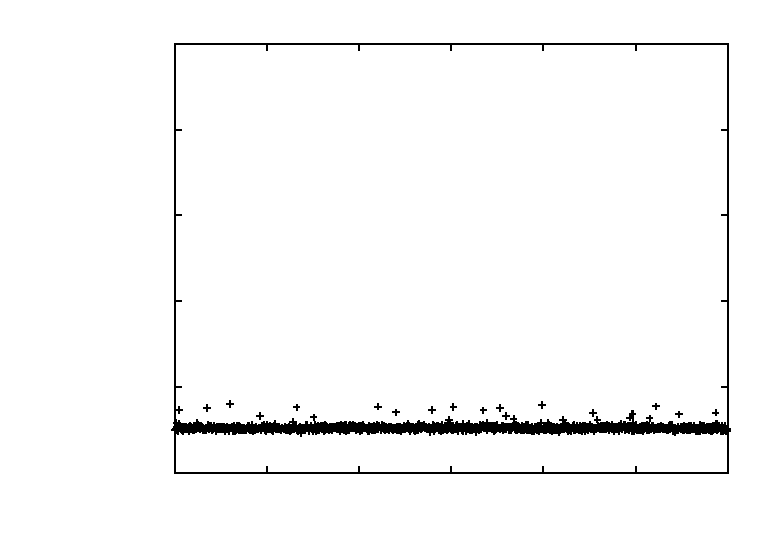
\includegraphics{fig/xenTot}}%
    \gplfronttext
  \end{picture}%
\endgroup
}}}
  \hspace{20pt}%
  \subfloat[][Escalonamento  - Com estresse]{%
    \label{fig:xenTotSched}%
    {\scalebox{0.84}{% GNUPLOT: LaTeX picture with Postscript
\begingroup
  \makeatletter
  \providecommand\color[2][]{%
    \GenericError{(gnuplot) \space\space\space\@spaces}{%
      Package color not loaded in conjunction with
      terminal option `colourtext'%
    }{See the gnuplot documentation for explanation.%
    }{Either use 'blacktext' in gnuplot or load the package
      color.sty in LaTeX.}%
    \renewcommand\color[2][]{}%
  }%
  \providecommand\includegraphics[2][]{%
    \GenericError{(gnuplot) \space\space\space\@spaces}{%
      Package graphicx or graphics not loaded%
    }{See the gnuplot documentation for explanation.%
    }{The gnuplot epslatex terminal needs graphicx.sty or graphics.sty.}%
    \renewcommand\includegraphics[2][]{}%
  }%
  \providecommand\rotatebox[2]{#2}%
  \@ifundefined{ifGPcolor}{%
    \newif\ifGPcolor
    \GPcolorfalse
  }{}%
  \@ifundefined{ifGPblacktext}{%
    \newif\ifGPblacktext
    \GPblacktextfalse
  }{}%
  % define a \g@addto@macro without @ in the name:
  \let\gplgaddtomacro\g@addto@macro
  % define empty templates for all commands taking text:
  \gdef\gplbacktext{}%
  \gdef\gplfronttext{}%
  \makeatother
  \ifGPblacktext
    % no textcolor at all
    \def\colorrgb#1{}%
    \def\colorgray#1{}%
  \else
    % gray or color?
    \ifGPcolor
      \def\colorrgb#1{\color[rgb]{#1}}%
      \def\colorgray#1{\color[gray]{#1}}%
      \expandafter\def\csname LTw\endcsname{\color{white}}%
      \expandafter\def\csname LTb\endcsname{\color{black}}%
      \expandafter\def\csname LTa\endcsname{\color{black}}%
      \expandafter\def\csname LT0\endcsname{\color[rgb]{1,0,0}}%
      \expandafter\def\csname LT1\endcsname{\color[rgb]{0,1,0}}%
      \expandafter\def\csname LT2\endcsname{\color[rgb]{0,0,1}}%
      \expandafter\def\csname LT3\endcsname{\color[rgb]{1,0,1}}%
      \expandafter\def\csname LT4\endcsname{\color[rgb]{0,1,1}}%
      \expandafter\def\csname LT5\endcsname{\color[rgb]{1,1,0}}%
      \expandafter\def\csname LT6\endcsname{\color[rgb]{0,0,0}}%
      \expandafter\def\csname LT7\endcsname{\color[rgb]{1,0.3,0}}%
      \expandafter\def\csname LT8\endcsname{\color[rgb]{0.5,0.5,0.5}}%
    \else
      % gray
      \def\colorrgb#1{\color{black}}%
      \def\colorgray#1{\color[gray]{#1}}%
      \expandafter\def\csname LTw\endcsname{\color{white}}%
      \expandafter\def\csname LTb\endcsname{\color{black}}%
      \expandafter\def\csname LTa\endcsname{\color{black}}%
      \expandafter\def\csname LT0\endcsname{\color{black}}%
      \expandafter\def\csname LT1\endcsname{\color{black}}%
      \expandafter\def\csname LT2\endcsname{\color{black}}%
      \expandafter\def\csname LT3\endcsname{\color{black}}%
      \expandafter\def\csname LT4\endcsname{\color{black}}%
      \expandafter\def\csname LT5\endcsname{\color{black}}%
      \expandafter\def\csname LT6\endcsname{\color{black}}%
      \expandafter\def\csname LT7\endcsname{\color{black}}%
      \expandafter\def\csname LT8\endcsname{\color{black}}%
    \fi
  \fi
  \setlength{\unitlength}{0.0500bp}%
  \begin{picture}(7200.00,5040.00)%
    \gplgaddtomacro\gplbacktext{%
      \csname LTb\endcsname%
      \put(1034,594){\makebox(0,0)[r]{\strut{}$0.0$}}%
      \put(1034,1291){\makebox(0,0)[r]{\strut{}$5.0$}}%
      \put(1034,1988){\makebox(0,0)[r]{\strut{}$10.0$}}%
      \put(1034,2685){\makebox(0,0)[r]{\strut{}$15.0$}}%
      \put(1034,3382){\makebox(0,0)[r]{\strut{}$20.0$}}%
      \put(1034,4079){\makebox(0,0)[r]{\strut{}$25.0$}}%
      \put(1034,4776){\makebox(0,0)[r]{\strut{}$30.0$}}%
      \put(1166,374){\makebox(0,0){\strut{}$ 0$}}%
      \put(2109,374){\makebox(0,0){\strut{}$ 10$}}%
      \put(3053,374){\makebox(0,0){\strut{}$ 20$}}%
      \put(3996,374){\makebox(0,0){\strut{}$ 30$}}%
      \put(4939,374){\makebox(0,0){\strut{}$ 40$}}%
      \put(5883,374){\makebox(0,0){\strut{}$ 50$}}%
      \put(6826,374){\makebox(0,0){\strut{}$ 60$}}%
      \put(396,2685){\rotatebox{90}{\makebox(0,0){\strut{}Lat\^encia em $\mu s$}}}%
      \put(3996,110){\makebox(0,0){\strut{}Tempo de observa\c{c}\~ao em $s$}}%
    }%
    \gplgaddtomacro\gplfronttext{%
    }%
    \gplbacktext
    \put(0,0){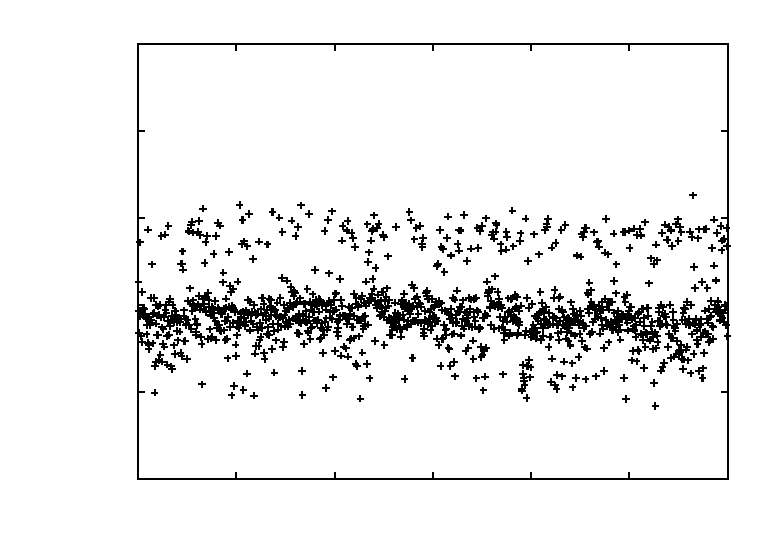
\includegraphics{fig2/xenTotSched}}%
    \gplfronttext
  \end{picture}%
\endgroup
}}}%

  \caption[Lat�ncia de interrup��o e de escalonamento do Xenomai-Linux]{Lat�ncia de
    interrup��o e de escalonamento do Xenomai 2.4-rc5 instalado no \kernell Linux,
    vers�o 2.6.19.7. As figuras \subref{fig:xenSem} e \subref{fig:xenSemSched}
    representam uma execu��o sem estresse e as figuras \subref{fig:xenTot} e
    \subref{fig:xenTotSched} representam uma execu��o com estresse do processador.
    A freq��ncia de escrita na porta paralela � de $20 Hz$.}
  \label{fig:xenoExp}%
\end{sidewaysfigure}


\begin{sidewaysfigure}
  \centering
  \subfloat[Interrup��o - Sem estresse]{%
    \label{fig:rtaiSem}%
    {\scalebox{0.84}{% GNUPLOT: LaTeX picture with Postscript
\begingroup
  \makeatletter
  \providecommand\color[2][]{%
    \GenericError{(gnuplot) \space\space\space\@spaces}{%
      Package color not loaded in conjunction with
      terminal option `colourtext'%
    }{See the gnuplot documentation for explanation.%
    }{Either use 'blacktext' in gnuplot or load the package
      color.sty in LaTeX.}%
    \renewcommand\color[2][]{}%
  }%
  \providecommand\includegraphics[2][]{%
    \GenericError{(gnuplot) \space\space\space\@spaces}{%
      Package graphicx or graphics not loaded%
    }{See the gnuplot documentation for explanation.%
    }{The gnuplot epslatex terminal needs graphicx.sty or graphics.sty.}%
    \renewcommand\includegraphics[2][]{}%
  }%
  \providecommand\rotatebox[2]{#2}%
  \@ifundefined{ifGPcolor}{%
    \newif\ifGPcolor
    \GPcolorfalse
  }{}%
  \@ifundefined{ifGPblacktext}{%
    \newif\ifGPblacktext
    \GPblacktexttrue
  }{}%
  % define a \g@addto@macro without @ in the name:
  \let\gplgaddtomacro\g@addto@macro
  % define empty templates for all commands taking text:
  \gdef\gplbacktext{}%
  \gdef\gplfronttext{}%
  \makeatother
  \ifGPblacktext
    % no textcolor at all
    \def\colorrgb#1{}%
    \def\colorgray#1{}%
  \else
    % gray or color?
    \ifGPcolor
      \def\colorrgb#1{\color[rgb]{#1}}%
      \def\colorgray#1{\color[gray]{#1}}%
      \expandafter\def\csname LTw\endcsname{\color{white}}%
      \expandafter\def\csname LTb\endcsname{\color{black}}%
      \expandafter\def\csname LTa\endcsname{\color{black}}%
      \expandafter\def\csname LT0\endcsname{\color[rgb]{1,0,0}}%
      \expandafter\def\csname LT1\endcsname{\color[rgb]{0,1,0}}%
      \expandafter\def\csname LT2\endcsname{\color[rgb]{0,0,1}}%
      \expandafter\def\csname LT3\endcsname{\color[rgb]{1,0,1}}%
      \expandafter\def\csname LT4\endcsname{\color[rgb]{0,1,1}}%
      \expandafter\def\csname LT5\endcsname{\color[rgb]{1,1,0}}%
      \expandafter\def\csname LT6\endcsname{\color[rgb]{0,0,0}}%
      \expandafter\def\csname LT7\endcsname{\color[rgb]{1,0.3,0}}%
      \expandafter\def\csname LT8\endcsname{\color[rgb]{0.5,0.5,0.5}}%
    \else
      % gray
      \def\colorrgb#1{\color{black}}%
      \def\colorgray#1{\color[gray]{#1}}%
      \expandafter\def\csname LTw\endcsname{\color{white}}%
      \expandafter\def\csname LTb\endcsname{\color{black}}%
      \expandafter\def\csname LTa\endcsname{\color{black}}%
      \expandafter\def\csname LT0\endcsname{\color{black}}%
      \expandafter\def\csname LT1\endcsname{\color{black}}%
      \expandafter\def\csname LT2\endcsname{\color{black}}%
      \expandafter\def\csname LT3\endcsname{\color{black}}%
      \expandafter\def\csname LT4\endcsname{\color{black}}%
      \expandafter\def\csname LT5\endcsname{\color{black}}%
      \expandafter\def\csname LT6\endcsname{\color{black}}%
      \expandafter\def\csname LT7\endcsname{\color{black}}%
      \expandafter\def\csname LT8\endcsname{\color{black}}%
    \fi
  \fi
  \setlength{\unitlength}{0.0500bp}%
  \begin{picture}(7200.00,5040.00)%
    \gplgaddtomacro\gplbacktext{%
      \csname LTb\endcsname%
      \put(1254,660){\makebox(0,0)[r]{\strut{}$5.0$}}%
      \put(1254,1346){\makebox(0,0)[r]{\strut{}$10.0$}}%
      \put(1254,2032){\makebox(0,0)[r]{\strut{}$15.0$}}%
      \put(1254,2718){\makebox(0,0)[r]{\strut{}$20.0$}}%
      \put(1254,3404){\makebox(0,0)[r]{\strut{}$25.0$}}%
      \put(1254,4090){\makebox(0,0)[r]{\strut{}$30.0$}}%
      \put(1254,4776){\makebox(0,0)[r]{\strut{}$35.0$}}%
      \put(1386,440){\makebox(0,0){\strut{}$ 0$}}%
      \put(2293,440){\makebox(0,0){\strut{}$ 10$}}%
      \put(3199,440){\makebox(0,0){\strut{}$ 20$}}%
      \put(4106,440){\makebox(0,0){\strut{}$ 30$}}%
      \put(5013,440){\makebox(0,0){\strut{}$ 40$}}%
      \put(5919,440){\makebox(0,0){\strut{}$ 50$}}%
      \put(6826,440){\makebox(0,0){\strut{}$ 60$}}%
      \put(220,2718){\rotatebox{90}{\makebox(0,0){\strut{}Lat\^encia em $\mu s$}}}%
      \put(4106,110){\makebox(0,0){\strut{}Tempo de observa\c{c}\~ao em $s$}}%
    }%
    \gplgaddtomacro\gplfronttext{%
    }%
    \gplbacktext
    \put(0,0){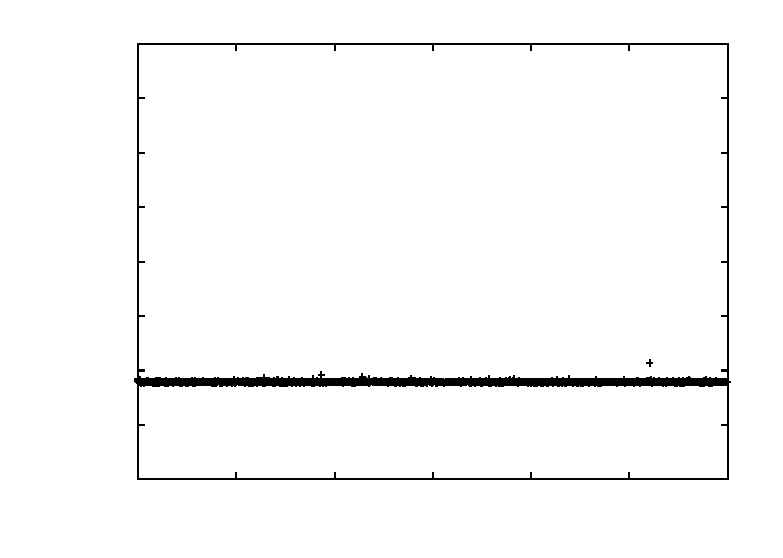
\includegraphics{fig/rtaiSem}}%
    \gplfronttext
  \end{picture}%
\endgroup
}}}
  \hspace{20pt}%
  \subfloat[][Escalonamento  - Sem estresse]{%
    \label{fig:rtaiSemSched}%
    {\scalebox{0.84}{% GNUPLOT: LaTeX picture with Postscript
\begingroup
  \makeatletter
  \providecommand\color[2][]{%
    \GenericError{(gnuplot) \space\space\space\@spaces}{%
      Package color not loaded in conjunction with
      terminal option `colourtext'%
    }{See the gnuplot documentation for explanation.%
    }{Either use 'blacktext' in gnuplot or load the package
      color.sty in LaTeX.}%
    \renewcommand\color[2][]{}%
  }%
  \providecommand\includegraphics[2][]{%
    \GenericError{(gnuplot) \space\space\space\@spaces}{%
      Package graphicx or graphics not loaded%
    }{See the gnuplot documentation for explanation.%
    }{The gnuplot epslatex terminal needs graphicx.sty or graphics.sty.}%
    \renewcommand\includegraphics[2][]{}%
  }%
  \providecommand\rotatebox[2]{#2}%
  \@ifundefined{ifGPcolor}{%
    \newif\ifGPcolor
    \GPcolorfalse
  }{}%
  \@ifundefined{ifGPblacktext}{%
    \newif\ifGPblacktext
    \GPblacktextfalse
  }{}%
  % define a \g@addto@macro without @ in the name:
  \let\gplgaddtomacro\g@addto@macro
  % define empty templates for all commands taking text:
  \gdef\gplbacktext{}%
  \gdef\gplfronttext{}%
  \makeatother
  \ifGPblacktext
    % no textcolor at all
    \def\colorrgb#1{}%
    \def\colorgray#1{}%
  \else
    % gray or color?
    \ifGPcolor
      \def\colorrgb#1{\color[rgb]{#1}}%
      \def\colorgray#1{\color[gray]{#1}}%
      \expandafter\def\csname LTw\endcsname{\color{white}}%
      \expandafter\def\csname LTb\endcsname{\color{black}}%
      \expandafter\def\csname LTa\endcsname{\color{black}}%
      \expandafter\def\csname LT0\endcsname{\color[rgb]{1,0,0}}%
      \expandafter\def\csname LT1\endcsname{\color[rgb]{0,1,0}}%
      \expandafter\def\csname LT2\endcsname{\color[rgb]{0,0,1}}%
      \expandafter\def\csname LT3\endcsname{\color[rgb]{1,0,1}}%
      \expandafter\def\csname LT4\endcsname{\color[rgb]{0,1,1}}%
      \expandafter\def\csname LT5\endcsname{\color[rgb]{1,1,0}}%
      \expandafter\def\csname LT6\endcsname{\color[rgb]{0,0,0}}%
      \expandafter\def\csname LT7\endcsname{\color[rgb]{1,0.3,0}}%
      \expandafter\def\csname LT8\endcsname{\color[rgb]{0.5,0.5,0.5}}%
    \else
      % gray
      \def\colorrgb#1{\color{black}}%
      \def\colorgray#1{\color[gray]{#1}}%
      \expandafter\def\csname LTw\endcsname{\color{white}}%
      \expandafter\def\csname LTb\endcsname{\color{black}}%
      \expandafter\def\csname LTa\endcsname{\color{black}}%
      \expandafter\def\csname LT0\endcsname{\color{black}}%
      \expandafter\def\csname LT1\endcsname{\color{black}}%
      \expandafter\def\csname LT2\endcsname{\color{black}}%
      \expandafter\def\csname LT3\endcsname{\color{black}}%
      \expandafter\def\csname LT4\endcsname{\color{black}}%
      \expandafter\def\csname LT5\endcsname{\color{black}}%
      \expandafter\def\csname LT6\endcsname{\color{black}}%
      \expandafter\def\csname LT7\endcsname{\color{black}}%
      \expandafter\def\csname LT8\endcsname{\color{black}}%
    \fi
  \fi
  \setlength{\unitlength}{0.0500bp}%
  \begin{picture}(7200.00,5040.00)%
    \gplgaddtomacro\gplbacktext{%
      \csname LTb\endcsname%
      \put(1034,594){\makebox(0,0)[r]{\strut{}$0.0$}}%
      \put(1034,1640){\makebox(0,0)[r]{\strut{}$5.0$}}%
      \put(1034,2685){\makebox(0,0)[r]{\strut{}$10.0$}}%
      \put(1034,3731){\makebox(0,0)[r]{\strut{}$15.0$}}%
      \put(1034,4776){\makebox(0,0)[r]{\strut{}$20.0$}}%
      \put(1166,374){\makebox(0,0){\strut{}$ 0$}}%
      \put(2109,374){\makebox(0,0){\strut{}$ 10$}}%
      \put(3053,374){\makebox(0,0){\strut{}$ 20$}}%
      \put(3996,374){\makebox(0,0){\strut{}$ 30$}}%
      \put(4939,374){\makebox(0,0){\strut{}$ 40$}}%
      \put(5883,374){\makebox(0,0){\strut{}$ 50$}}%
      \put(6826,374){\makebox(0,0){\strut{}$ 60$}}%
      \put(396,2685){\rotatebox{90}{\makebox(0,0){\strut{}Latency ($\mu s$)}}}%
      \put(3996,110){\makebox(0,0){\strut{}Time ($s$)}}%
    }%
    \gplgaddtomacro\gplfronttext{%
    }%
    \gplbacktext
    \put(0,0){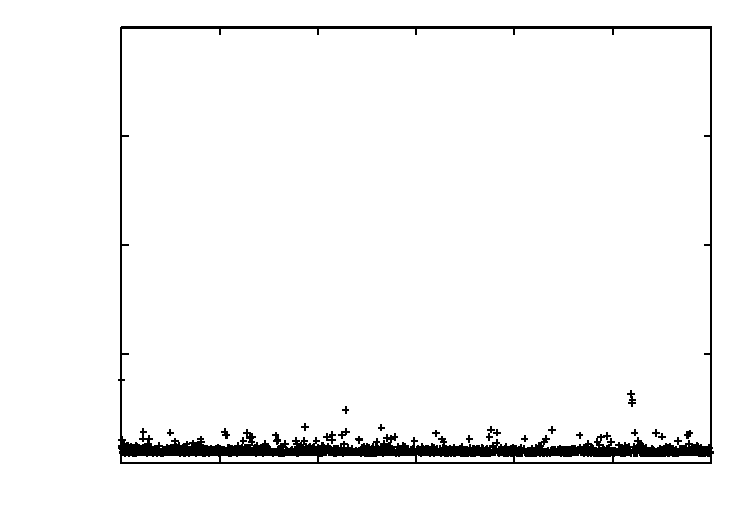
\includegraphics{fig/rtaiSemSched.pdf}}%
    \gplfronttext
  \end{picture}%
\endgroup
}}}\\%
%   \hspace{14pt}%
  \subfloat[Interrup��o - Com estresse]{%
    \label{fig:rtaiTot}%
    {\scalebox{0.84}{% GNUPLOT: LaTeX picture with Postscript
\begingroup
  \makeatletter
  \providecommand\color[2][]{%
    \GenericError{(gnuplot) \space\space\space\@spaces}{%
      Package color not loaded in conjunction with
      terminal option `colourtext'%
    }{See the gnuplot documentation for explanation.%
    }{Either use 'blacktext' in gnuplot or load the package
      color.sty in LaTeX.}%
    \renewcommand\color[2][]{}%
  }%
  \providecommand\includegraphics[2][]{%
    \GenericError{(gnuplot) \space\space\space\@spaces}{%
      Package graphicx or graphics not loaded%
    }{See the gnuplot documentation for explanation.%
    }{The gnuplot epslatex terminal needs graphicx.sty or graphics.sty.}%
    \renewcommand\includegraphics[2][]{}%
  }%
  \providecommand\rotatebox[2]{#2}%
  \@ifundefined{ifGPcolor}{%
    \newif\ifGPcolor
    \GPcolorfalse
  }{}%
  \@ifundefined{ifGPblacktext}{%
    \newif\ifGPblacktext
    \GPblacktextfalse
  }{}%
  % define a \g@addto@macro without @ in the name:
  \let\gplgaddtomacro\g@addto@macro
  % define empty templates for all commands taking text:
  \gdef\gplbacktext{}%
  \gdef\gplfronttext{}%
  \makeatother
  \ifGPblacktext
    % no textcolor at all
    \def\colorrgb#1{}%
    \def\colorgray#1{}%
  \else
    % gray or color?
    \ifGPcolor
      \def\colorrgb#1{\color[rgb]{#1}}%
      \def\colorgray#1{\color[gray]{#1}}%
      \expandafter\def\csname LTw\endcsname{\color{white}}%
      \expandafter\def\csname LTb\endcsname{\color{black}}%
      \expandafter\def\csname LTa\endcsname{\color{black}}%
      \expandafter\def\csname LT0\endcsname{\color[rgb]{1,0,0}}%
      \expandafter\def\csname LT1\endcsname{\color[rgb]{0,1,0}}%
      \expandafter\def\csname LT2\endcsname{\color[rgb]{0,0,1}}%
      \expandafter\def\csname LT3\endcsname{\color[rgb]{1,0,1}}%
      \expandafter\def\csname LT4\endcsname{\color[rgb]{0,1,1}}%
      \expandafter\def\csname LT5\endcsname{\color[rgb]{1,1,0}}%
      \expandafter\def\csname LT6\endcsname{\color[rgb]{0,0,0}}%
      \expandafter\def\csname LT7\endcsname{\color[rgb]{1,0.3,0}}%
      \expandafter\def\csname LT8\endcsname{\color[rgb]{0.5,0.5,0.5}}%
    \else
      % gray
      \def\colorrgb#1{\color{black}}%
      \def\colorgray#1{\color[gray]{#1}}%
      \expandafter\def\csname LTw\endcsname{\color{white}}%
      \expandafter\def\csname LTb\endcsname{\color{black}}%
      \expandafter\def\csname LTa\endcsname{\color{black}}%
      \expandafter\def\csname LT0\endcsname{\color{black}}%
      \expandafter\def\csname LT1\endcsname{\color{black}}%
      \expandafter\def\csname LT2\endcsname{\color{black}}%
      \expandafter\def\csname LT3\endcsname{\color{black}}%
      \expandafter\def\csname LT4\endcsname{\color{black}}%
      \expandafter\def\csname LT5\endcsname{\color{black}}%
      \expandafter\def\csname LT6\endcsname{\color{black}}%
      \expandafter\def\csname LT7\endcsname{\color{black}}%
      \expandafter\def\csname LT8\endcsname{\color{black}}%
    \fi
  \fi
  \setlength{\unitlength}{0.0500bp}%
  \begin{picture}(7200.00,5040.00)%
    \gplgaddtomacro\gplbacktext{%
      \csname LTb\endcsname%
      \put(1034,594){\makebox(0,0)[r]{\strut{}$0.0$}}%
      \put(1034,1117){\makebox(0,0)[r]{\strut{}$5.0$}}%
      \put(1034,1640){\makebox(0,0)[r]{\strut{}$10.0$}}%
      \put(1034,2162){\makebox(0,0)[r]{\strut{}$15.0$}}%
      \put(1034,2685){\makebox(0,0)[r]{\strut{}$20.0$}}%
      \put(1034,3208){\makebox(0,0)[r]{\strut{}$25.0$}}%
      \put(1034,3731){\makebox(0,0)[r]{\strut{}$30.0$}}%
      \put(1034,4253){\makebox(0,0)[r]{\strut{}$35.0$}}%
      \put(1034,4776){\makebox(0,0)[r]{\strut{}$40.0$}}%
      \put(1166,374){\makebox(0,0){\strut{}$ 0$}}%
      \put(2109,374){\makebox(0,0){\strut{}$ 10$}}%
      \put(3053,374){\makebox(0,0){\strut{}$ 20$}}%
      \put(3996,374){\makebox(0,0){\strut{}$ 30$}}%
      \put(4939,374){\makebox(0,0){\strut{}$ 40$}}%
      \put(5883,374){\makebox(0,0){\strut{}$ 50$}}%
      \put(6826,374){\makebox(0,0){\strut{}$ 60$}}%
      \put(396,2685){\rotatebox{90}{\makebox(0,0){\strut{}Lat\^encia em $\mu s$}}}%
      \put(3996,110){\makebox(0,0){\strut{}Tempo de observa\c{c}\~ao em $s$}}%
    }%
    \gplgaddtomacro\gplfronttext{%
    }%
    \gplbacktext
    \put(0,0){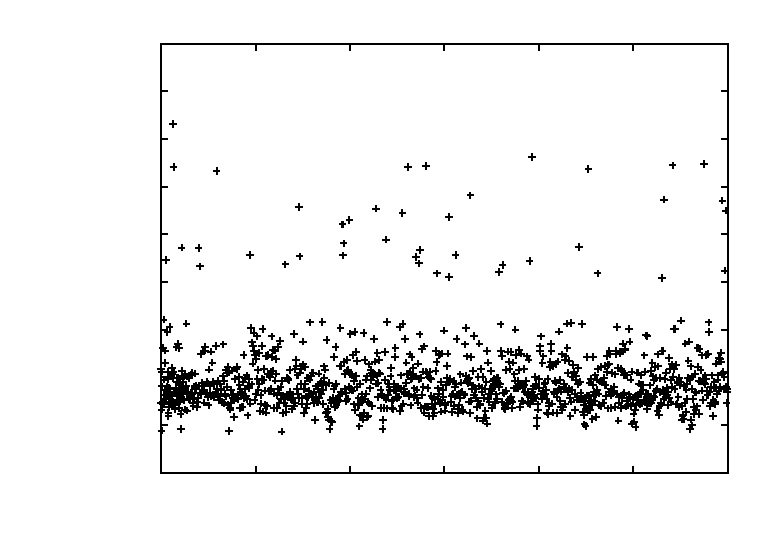
\includegraphics{fig/rtaiTot}}%
    \gplfronttext
  \end{picture}%
\endgroup
}}}
  \hspace{20pt}%
  \subfloat[][Escalonamento  - Com estresse]{%
    \label{fig:rtaiTotSched}%
    {\scalebox{0.84}{% GNUPLOT: LaTeX picture with Postscript
\begingroup
  \makeatletter
  \providecommand\color[2][]{%
    \GenericError{(gnuplot) \space\space\space\@spaces}{%
      Package color not loaded in conjunction with
      terminal option `colourtext'%
    }{See the gnuplot documentation for explanation.%
    }{Either use 'blacktext' in gnuplot or load the package
      color.sty in LaTeX.}%
    \renewcommand\color[2][]{}%
  }%
  \providecommand\includegraphics[2][]{%
    \GenericError{(gnuplot) \space\space\space\@spaces}{%
      Package graphicx or graphics not loaded%
    }{See the gnuplot documentation for explanation.%
    }{The gnuplot epslatex terminal needs graphicx.sty or graphics.sty.}%
    \renewcommand\includegraphics[2][]{}%
  }%
  \providecommand\rotatebox[2]{#2}%
  \@ifundefined{ifGPcolor}{%
    \newif\ifGPcolor
    \GPcolorfalse
  }{}%
  \@ifundefined{ifGPblacktext}{%
    \newif\ifGPblacktext
    \GPblacktextfalse
  }{}%
  % define a \g@addto@macro without @ in the name:
  \let\gplgaddtomacro\g@addto@macro
  % define empty templates for all commands taking text:
  \gdef\gplbacktext{}%
  \gdef\gplfronttext{}%
  \makeatother
  \ifGPblacktext
    % no textcolor at all
    \def\colorrgb#1{}%
    \def\colorgray#1{}%
  \else
    % gray or color?
    \ifGPcolor
      \def\colorrgb#1{\color[rgb]{#1}}%
      \def\colorgray#1{\color[gray]{#1}}%
      \expandafter\def\csname LTw\endcsname{\color{white}}%
      \expandafter\def\csname LTb\endcsname{\color{black}}%
      \expandafter\def\csname LTa\endcsname{\color{black}}%
      \expandafter\def\csname LT0\endcsname{\color[rgb]{1,0,0}}%
      \expandafter\def\csname LT1\endcsname{\color[rgb]{0,1,0}}%
      \expandafter\def\csname LT2\endcsname{\color[rgb]{0,0,1}}%
      \expandafter\def\csname LT3\endcsname{\color[rgb]{1,0,1}}%
      \expandafter\def\csname LT4\endcsname{\color[rgb]{0,1,1}}%
      \expandafter\def\csname LT5\endcsname{\color[rgb]{1,1,0}}%
      \expandafter\def\csname LT6\endcsname{\color[rgb]{0,0,0}}%
      \expandafter\def\csname LT7\endcsname{\color[rgb]{1,0.3,0}}%
      \expandafter\def\csname LT8\endcsname{\color[rgb]{0.5,0.5,0.5}}%
    \else
      % gray
      \def\colorrgb#1{\color{black}}%
      \def\colorgray#1{\color[gray]{#1}}%
      \expandafter\def\csname LTw\endcsname{\color{white}}%
      \expandafter\def\csname LTb\endcsname{\color{black}}%
      \expandafter\def\csname LTa\endcsname{\color{black}}%
      \expandafter\def\csname LT0\endcsname{\color{black}}%
      \expandafter\def\csname LT1\endcsname{\color{black}}%
      \expandafter\def\csname LT2\endcsname{\color{black}}%
      \expandafter\def\csname LT3\endcsname{\color{black}}%
      \expandafter\def\csname LT4\endcsname{\color{black}}%
      \expandafter\def\csname LT5\endcsname{\color{black}}%
      \expandafter\def\csname LT6\endcsname{\color{black}}%
      \expandafter\def\csname LT7\endcsname{\color{black}}%
      \expandafter\def\csname LT8\endcsname{\color{black}}%
    \fi
  \fi
  \setlength{\unitlength}{0.0500bp}%
  \begin{picture}(7200.00,5040.00)%
    \gplgaddtomacro\gplbacktext{%
      \csname LTb\endcsname%
      \put(1034,594){\makebox(0,0)[r]{\strut{}$0.0$}}%
      \put(1034,1640){\makebox(0,0)[r]{\strut{}$5.0$}}%
      \put(1034,2685){\makebox(0,0)[r]{\strut{}$10.0$}}%
      \put(1034,3731){\makebox(0,0)[r]{\strut{}$15.0$}}%
      \put(1034,4776){\makebox(0,0)[r]{\strut{}$20.0$}}%
      \put(1166,374){\makebox(0,0){\strut{}$ 0$}}%
      \put(2109,374){\makebox(0,0){\strut{}$ 10$}}%
      \put(3053,374){\makebox(0,0){\strut{}$ 20$}}%
      \put(3996,374){\makebox(0,0){\strut{}$ 30$}}%
      \put(4939,374){\makebox(0,0){\strut{}$ 40$}}%
      \put(5883,374){\makebox(0,0){\strut{}$ 50$}}%
      \put(6826,374){\makebox(0,0){\strut{}$ 60$}}%
      \put(396,2685){\rotatebox{90}{\makebox(0,0){\strut{}Lat\^encia em $\mu s$}}}%
      \put(3996,110){\makebox(0,0){\strut{}Tempo de observa\c{c}\~ao em $s$}}%
    }%
    \gplgaddtomacro\gplfronttext{%
    }%
    \gplbacktext
    \put(0,0){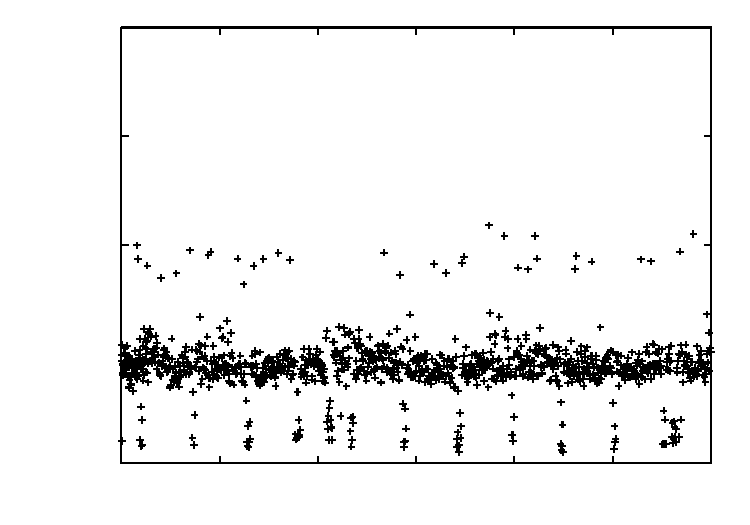
\includegraphics{fig/rtaiTotSched.pdf}}%
    \gplfronttext
  \end{picture}%
\endgroup
}}}%

  \caption[Lat�ncia de interrup��o e de escalonamento do RTAI-Linux]{Lat�ncia de
    interrup��o e de escalonamento do RTAI magma instalado no \kernell Linux, vers�o
    2.6.19.7.  As figuras \subref{fig:rtaiSem} e \subref{fig:rtaiSemSched}
    representam uma execu��o sem estresse e as figuras \subref{fig:rtaiTot} e
    \subref{fig:rtaiTotSched} representam uma execu��o com estresse do processador.
    A freq��ncia de escrita na porta paralela � de $20 Hz$.}
  \label{fig:rtaiExp}%
\end{sidewaysfigure}



\begin{comment}

\subsection{Modo operacional}
\label{sec:modOp}

Para realizar as medidas de lat�ncia de interrup��o e de tratamento, o processo $P$
executou escritas no pino 9 da porta paralela com uma freq��ncia aproximada de $20
Hz$. J� que as medidas n�o dependem do valor do instante inicial da escrita, esta
freq��ncia foi obtida utilizando uma chamada a fun��o \cod{sleep} com um argumento
de $50 ms$.  Esta freq��ncia relativamente baixa foi escolhida para garantir o
processamento completo de todas as opera��es de medida e o escalonamento eventual de
outros processos entre cada escrita na porta paralela.  No entanto, resultados
quantitativamente id�nticos ser�o mostrados na se��o \ref{} para o RTAI e o Xenomai
com uma freq��ncia de $1000 Hz$.

No caso destas duas plataformas, RTAI e do Xenomai, o foco foi dado a lat�ncia de
interrup��o associadas ao dom�nio prim�rio, descrito na se��o \ref{sec:adeos}, j�
que a proposta do protocolo \doriss � oferecer garantias temporais para tarefas de
tempo real cr�ticas.

Cada um dos cen�rios de medida durou aproximadamente 70 segundos e foi realizados
usando um ambiente gr�fico. No entanto, experimentos em modo \ing{single}, no qual o
n�mero de \ing{thread} de \kernell � m�nimo, deram os mesmos resultados
quantitativos. Nos primeiros 10 segundos dos experimentos, o processo $P$ gerou as
interrup��es na freq��ncia de $20 Hz$ sem que nenhum outra atividade interfere.

Entre a d�cima e a vig�sima segunda, um estresse de comunica��o foi aplicado ao
sistema via a rede Ethernet durante aproximadamente 10 segundos. O estresse aplicado
utilizou o comando \cod{ssh} da seguinte maneira. Uma m�quina remota executou o
comando \ing{shell} \cod{ssh IP "echo \$ITER >> /tmp/stress"}, 60 vezes
consecutivas.  Nesta express�o, $IP$ era o n�mero IP da esta��o na qual as medidas
eram realizadas e $\$ITER$ era o �ndice de itera��o do la�o de execu��o do
comando. Constatou-se que 60 vezes corespondiam aproximadamente a um tempo de
execu��o de 10 segundos.

A escolha deste tipo de estresse se justificou por duas raz�es principais.  Em
primeiro lugar, a placa de rede utiliza a linha de interrup��o 18 cuja prioridade �
menor que a prioridade da porta paralela. Portanto, as interrup��es geradas nesta
pela placa de rede n�o deveriam interferir a princ�pios nas medidas efetuadas.  Em
segundo lugar, j� que este trabalho tem por objetivo a implementa��o de um protocolo
de rede baseado em Ethernet, pude-se avaliar a capacidade das diferentes plataformas
em garantir uma lat�ncia determin�stica no tratamento das interrup��es, mesmo na
presen�a de um estresse de comunica��o.

Todos os experimentos foram realizados pelo menos tr�s vezes e selecionou-se
os cen�rios com as lat�ncias maiores no pior caso.

% Este estresse foi criado simplesmente, utilizando uma comunica��o UDP do tipo
% cliente-servidor. Para gerar as interrup��es no computador no qual as medidas eram
% efetuadas, confi\-gurou-se este como servidor da comunica��o UDP. O processo servidor
% foi criado utilizando a API das bibliotecas \cod{pthread} com a prioridade mais
% alta poss�vel. O cliente, instalado numa m�quina remota, foi configurado para 
% transmitir pequenos pacotes de 64 \ing{bytes} na freq��ncia m�xima permitida pela
% rede, ou seja, com uma freq��ncia de quase $200 kHz$ (um pacote a cada $5 \mu s$).
% Desta forma, 200.000 interrup��es por segundos aconteciam na placa de rede
% do servidor.

\subsection{Resultados experimentais}
\label{sec:resulExp}

O dispositivo experimental descrito nas se��es \ref{sec:dispExp} e \ref{sec:modOp}
foi implementado em computadores Pentium 4 com processadores de 2.4 Ghz e 512 Mb de
mem�ria. Os resultados experimentais s�o apresentados pelo meio de figuras nas quais
o eixo horizontal representa o tempo variando de 0 a 70 segundos e o eixo vertical
representa a lat�ncia de interrup��o em $\mu s$ medida a cada escrita na porta
paralela. 

As seguintes configura��es das quatro plataformas Linux, PREEMP-RT, RTAI e Xenomai
foram utilizadas. A vers�o do \kernell de Linux 2.6.19.7 foi utilizada para os
testes do \kernell Linux, de RTAI e de Xenomai \cite{kernel}. Nos tr�s casos,
compilou-se o \kernell Linux com a configura��o de preemp��o habilitada
(\ing{Low-Latency}). Apesar de existir vers�es do \kernell mais recentes suportadas
por estas tr�s plataformas, RTAI e Xenomai disponibilizavam \ing{patchs} est�veis
para esta vers�o do \kernell no in�cio deste trabalho, em janeiro de 2007. J� que
estas duas plataformas s�o baseados no Adeos, como foi visto na descri��o da se��o
\ref{sec:adeos}, suas propriedades temporais n�o dependem, a princ�pio, do \kernel
Linux. Considerou-se ent�o desnecess�rio atualizar a vers�o do \kernell. No entanto,
utilizou-se as vers�es mais recentes das duas distribui��es do RTAI e Xenomai. No
caso do RTAI, a vers�o \ing{magma} foi baixada diretamente do site \cite{RTAI},
utilizando o sistema de controle de vers�o \ing{CVS}. Para o Xenomai, utilizou-se a
vers�o 2.4-rc5 dispon�vel desde outubro 2007 \cite{Xenomai}.

Para estas duas plataformas, os diferentes testes de lat�ncias fornecidos foram
utilizados, dando resultados de menos de $10 \mu s$ no pior caso para a lat�ncia de
interrup��o, conforme os padr�es da arquitetura Intel Pentium 4. Observa-se que, em
ambas plataformas, desabilitou-se as interrup��es de gerenciamento do sistema
(\ing{SMI}), conforme as recomenda��es dos desenvolvedores \cite{RTAI,
  Xenomai}. Isto permitiu cancelar uma lat�ncia da ordem de $2.5ms$ que aparecia nos
testes periodicamente a cada 32 segundos. No caso do Linux e de PREEMP-RT, as
interrup��es de gerenciamento do sistema n�o foram desabilitadas. No entanto, n�o se
observou nenhuma lat�ncia da ordem de $2.5ms$ nos experimentos relativos a estas duas
plataformas. Provavelmente, porque a interrup��o peri�dica de SMI aconteceu num
intervalo de tempo sem medida.

Em rela��o ao \ing{patch} PREEMPT-RT, ele tem evolu�do rapidamente no decorrer do
seus dois anos de vida. Notadamente, desde a vers�o 2.6.21, o \kernell Linux
disponibiliza temporizadores de alta precis�o para as arquiteturas x86, ARM e PPC, o
que permite ao \ing{patch} \preemptt de trabalhar com resolu��o da ordem do $\mu s$
(ver se��o \ref{sec:preemptRT}) no escalonamento de tarefas. Portanto, utilizou-se a
vers�o est�vel do \kernell em dezembro de 2007, isto �, a vers�o 2.6.23.9.

\subsubsection{Linux e \preempt}

\begin{figure}%
  \centering
  \subfloat[][Os tri�ngulos vermelhos correspondem aos piores casos.]{%
    \label{fig:klight1}%
    {\scalebox{1}{% GNUPLOT: LaTeX picture with Postscript
\begingroup
  \makeatletter
  \providecommand\color[2][]{%
    \GenericError{(gnuplot) \space\space\space\@spaces}{%
      Package color not loaded in conjunction with
      terminal option `colourtext'%
    }{See the gnuplot documentation for explanation.%
    }{Either use 'blacktext' in gnuplot or load the package
      color.sty in LaTeX.}%
    \renewcommand\color[2][]{}%
  }%
  \providecommand\includegraphics[2][]{%
    \GenericError{(gnuplot) \space\space\space\@spaces}{%
      Package graphicx or graphics not loaded%
    }{See the gnuplot documentation for explanation.%
    }{The gnuplot epslatex terminal needs graphicx.sty or graphics.sty.}%
    \renewcommand\includegraphics[2][]{}%
  }%
  \providecommand\rotatebox[2]{#2}%
  \@ifundefined{ifGPcolor}{%
    \newif\ifGPcolor
    \GPcolorfalse
  }{}%
  \@ifundefined{ifGPblacktext}{%
    \newif\ifGPblacktext
    \GPblacktextfalse
  }{}%
  % define a \g@addto@macro without @ in the name:
  \let\gplgaddtomacro\g@addto@macro
  % define empty templates for all commands taking text:
  \gdef\gplbacktext{}%
  \gdef\gplfronttext{}%
  \makeatother
  \ifGPblacktext
    % no textcolor at all
    \def\colorrgb#1{}%
    \def\colorgray#1{}%
  \else
    % gray or color?
    \ifGPcolor
      \def\colorrgb#1{\color[rgb]{#1}}%
      \def\colorgray#1{\color[gray]{#1}}%
      \expandafter\def\csname LTw\endcsname{\color{white}}%
      \expandafter\def\csname LTb\endcsname{\color{black}}%
      \expandafter\def\csname LTa\endcsname{\color{black}}%
      \expandafter\def\csname LT0\endcsname{\color[rgb]{1,0,0}}%
      \expandafter\def\csname LT1\endcsname{\color[rgb]{0,1,0}}%
      \expandafter\def\csname LT2\endcsname{\color[rgb]{0,0,1}}%
      \expandafter\def\csname LT3\endcsname{\color[rgb]{1,0,1}}%
      \expandafter\def\csname LT4\endcsname{\color[rgb]{0,1,1}}%
      \expandafter\def\csname LT5\endcsname{\color[rgb]{1,1,0}}%
      \expandafter\def\csname LT6\endcsname{\color[rgb]{0,0,0}}%
      \expandafter\def\csname LT7\endcsname{\color[rgb]{1,0.3,0}}%
      \expandafter\def\csname LT8\endcsname{\color[rgb]{0.5,0.5,0.5}}%
    \else
      % gray
      \def\colorrgb#1{\color{black}}%
      \def\colorgray#1{\color[gray]{#1}}%
      \expandafter\def\csname LTw\endcsname{\color{white}}%
      \expandafter\def\csname LTb\endcsname{\color{black}}%
      \expandafter\def\csname LTa\endcsname{\color{black}}%
      \expandafter\def\csname LT0\endcsname{\color{black}}%
      \expandafter\def\csname LT1\endcsname{\color{black}}%
      \expandafter\def\csname LT2\endcsname{\color{black}}%
      \expandafter\def\csname LT3\endcsname{\color{black}}%
      \expandafter\def\csname LT4\endcsname{\color{black}}%
      \expandafter\def\csname LT5\endcsname{\color{black}}%
      \expandafter\def\csname LT6\endcsname{\color{black}}%
      \expandafter\def\csname LT7\endcsname{\color{black}}%
      \expandafter\def\csname LT8\endcsname{\color{black}}%
    \fi
  \fi
  \setlength{\unitlength}{0.0500bp}%
  \begin{picture}(7200.00,5040.00)%
    \gplgaddtomacro\gplbacktext{%
      \csname LTb\endcsname%
      \put(1518,660){\makebox(0,0)[r]{\strut{}$0.0$}}%
      \put(1518,1175){\makebox(0,0)[r]{\strut{}$1000.0$}}%
      \put(1518,1689){\makebox(0,0)[r]{\strut{}$2000.0$}}%
      \put(1518,2204){\makebox(0,0)[r]{\strut{}$3000.0$}}%
      \put(1518,2718){\makebox(0,0)[r]{\strut{}$4000.0$}}%
      \put(1518,3233){\makebox(0,0)[r]{\strut{}$5000.0$}}%
      \put(1518,3747){\makebox(0,0)[r]{\strut{}$6000.0$}}%
      \put(1518,4262){\makebox(0,0)[r]{\strut{}$7000.0$}}%
      \put(1518,4776){\makebox(0,0)[r]{\strut{}$8000.0$}}%
      \put(1650,440){\makebox(0,0){\strut{}$ 0$}}%
      \put(2389,440){\makebox(0,0){\strut{}$ 10$}}%
      \put(3129,440){\makebox(0,0){\strut{}$ 20$}}%
      \put(3868,440){\makebox(0,0){\strut{}$ 30$}}%
      \put(4608,440){\makebox(0,0){\strut{}$ 40$}}%
      \put(5347,440){\makebox(0,0){\strut{}$ 50$}}%
      \put(6087,440){\makebox(0,0){\strut{}$ 60$}}%
      \put(6826,440){\makebox(0,0){\strut{}$ 70$}}%
      \put(220,2718){\rotatebox{90}{\makebox(0,0){\strut{}Lat\^encia em $\mu s$}}}%
      \put(4238,110){\makebox(0,0){\strut{}Tempo de execu\c{c}\~ao em $s$}}%
    }%
    \gplgaddtomacro\gplfronttext{%
    }%
    \gplbacktext
    \put(0,0){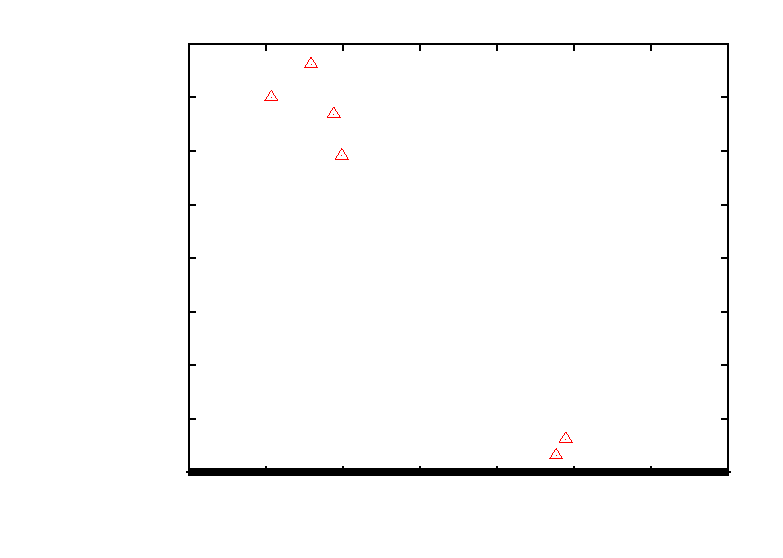
\includegraphics{fig/klight1}}%
    \gplfronttext
  \end{picture}%
\endgroup
}}}\\
  \vspace{10pt}%
  \subfloat[][Os piores casos s�o representados no valor $15 \mu s$.]{%
    \label{fig:klight2}%
    {\scalebox{1}{% GNUPLOT: LaTeX picture with Postscript
\begingroup
  \makeatletter
  \providecommand\color[2][]{%
    \GenericError{(gnuplot) \space\space\space\@spaces}{%
      Package color not loaded in conjunction with
      terminal option `colourtext'%
    }{See the gnuplot documentation for explanation.%
    }{Either use 'blacktext' in gnuplot or load the package
      color.sty in LaTeX.}%
    \renewcommand\color[2][]{}%
  }%
  \providecommand\includegraphics[2][]{%
    \GenericError{(gnuplot) \space\space\space\@spaces}{%
      Package graphicx or graphics not loaded%
    }{See the gnuplot documentation for explanation.%
    }{The gnuplot epslatex terminal needs graphicx.sty or graphics.sty.}%
    \renewcommand\includegraphics[2][]{}%
  }%
  \providecommand\rotatebox[2]{#2}%
  \@ifundefined{ifGPcolor}{%
    \newif\ifGPcolor
    \GPcolorfalse
  }{}%
  \@ifundefined{ifGPblacktext}{%
    \newif\ifGPblacktext
    \GPblacktextfalse
  }{}%
  % define a \g@addto@macro without @ in the name:
  \let\gplgaddtomacro\g@addto@macro
  % define empty templates for all commands taking text:
  \gdef\gplbacktext{}%
  \gdef\gplfronttext{}%
  \makeatother
  \ifGPblacktext
    % no textcolor at all
    \def\colorrgb#1{}%
    \def\colorgray#1{}%
  \else
    % gray or color?
    \ifGPcolor
      \def\colorrgb#1{\color[rgb]{#1}}%
      \def\colorgray#1{\color[gray]{#1}}%
      \expandafter\def\csname LTw\endcsname{\color{white}}%
      \expandafter\def\csname LTb\endcsname{\color{black}}%
      \expandafter\def\csname LTa\endcsname{\color{black}}%
      \expandafter\def\csname LT0\endcsname{\color[rgb]{1,0,0}}%
      \expandafter\def\csname LT1\endcsname{\color[rgb]{0,1,0}}%
      \expandafter\def\csname LT2\endcsname{\color[rgb]{0,0,1}}%
      \expandafter\def\csname LT3\endcsname{\color[rgb]{1,0,1}}%
      \expandafter\def\csname LT4\endcsname{\color[rgb]{0,1,1}}%
      \expandafter\def\csname LT5\endcsname{\color[rgb]{1,1,0}}%
      \expandafter\def\csname LT6\endcsname{\color[rgb]{0,0,0}}%
      \expandafter\def\csname LT7\endcsname{\color[rgb]{1,0.3,0}}%
      \expandafter\def\csname LT8\endcsname{\color[rgb]{0.5,0.5,0.5}}%
    \else
      % gray
      \def\colorrgb#1{\color{black}}%
      \def\colorgray#1{\color[gray]{#1}}%
      \expandafter\def\csname LTw\endcsname{\color{white}}%
      \expandafter\def\csname LTb\endcsname{\color{black}}%
      \expandafter\def\csname LTa\endcsname{\color{black}}%
      \expandafter\def\csname LT0\endcsname{\color{black}}%
      \expandafter\def\csname LT1\endcsname{\color{black}}%
      \expandafter\def\csname LT2\endcsname{\color{black}}%
      \expandafter\def\csname LT3\endcsname{\color{black}}%
      \expandafter\def\csname LT4\endcsname{\color{black}}%
      \expandafter\def\csname LT5\endcsname{\color{black}}%
      \expandafter\def\csname LT6\endcsname{\color{black}}%
      \expandafter\def\csname LT7\endcsname{\color{black}}%
      \expandafter\def\csname LT8\endcsname{\color{black}}%
    \fi
  \fi
  \setlength{\unitlength}{0.0500bp}%
  \begin{picture}(7200.00,5040.00)%
    \gplgaddtomacro\gplbacktext{%
      \csname LTb\endcsname%
      \put(1254,660){\makebox(0,0)[r]{\strut{}$8.0$}}%
      \put(1254,1175){\makebox(0,0)[r]{\strut{}$9.0$}}%
      \put(1254,1689){\makebox(0,0)[r]{\strut{}$10.0$}}%
      \put(1254,2204){\makebox(0,0)[r]{\strut{}$11.0$}}%
      \put(1254,2718){\makebox(0,0)[r]{\strut{}$12.0$}}%
      \put(1254,3233){\makebox(0,0)[r]{\strut{}$13.0$}}%
      \put(1254,3747){\makebox(0,0)[r]{\strut{}$14.0$}}%
      \put(1254,4262){\makebox(0,0)[r]{\strut{}$15.0$}}%
      \put(1254,4776){\makebox(0,0)[r]{\strut{}$16.0$}}%
      \put(1386,440){\makebox(0,0){\strut{}$ 0$}}%
      \put(2163,440){\makebox(0,0){\strut{}$ 10$}}%
      \put(2940,440){\makebox(0,0){\strut{}$ 20$}}%
      \put(3717,440){\makebox(0,0){\strut{}$ 30$}}%
      \put(4495,440){\makebox(0,0){\strut{}$ 40$}}%
      \put(5272,440){\makebox(0,0){\strut{}$ 50$}}%
      \put(6049,440){\makebox(0,0){\strut{}$ 60$}}%
      \put(6826,440){\makebox(0,0){\strut{}$ 70$}}%
      \put(220,2718){\rotatebox{90}{\makebox(0,0){\strut{}Lat\^encia em $\mu s$}}}%
      \put(4106,110){\makebox(0,0){\strut{}Tempo de execu\c{c}\~ao em $s$}}%
    }%
    \gplgaddtomacro\gplfronttext{%
    }%
    \gplbacktext
    \put(0,0){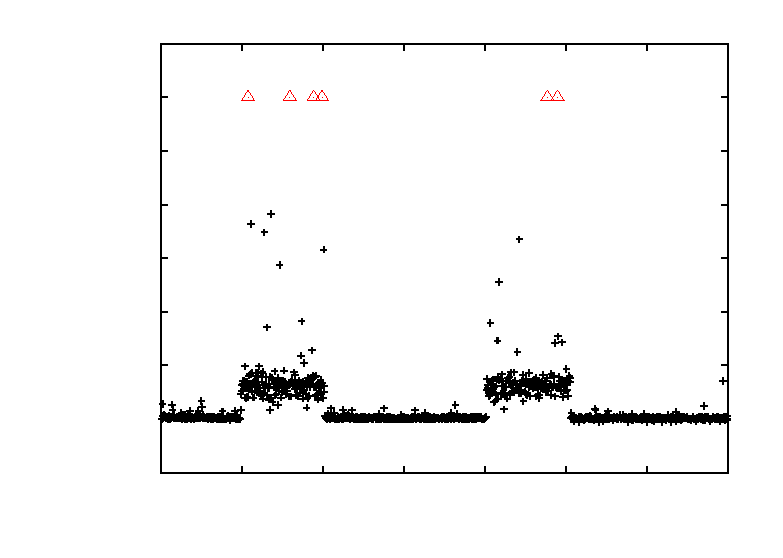
\includegraphics{fig/klight2}}%
    \gplfronttext
  \end{picture}%
\endgroup
}}}%
  \caption[Lat�ncia de interrup��o do Kernel Linux]{Lat�ncia de interrup��o do
    \kernell Linux 2.6.19.7, op��o \ing{Low-Latency}. As figuras
    \subref{fig:klight1} e \subref{fig:klight2} representam a mesma execu��o.  A
    freq��ncia de interrup��o de $20 Hz$ e os dois estresses (60 aberturas e
    fechamento de sess�o \cod{ssh}) s�o aplicados nos instantes 10s e 40s.  Na
    figura \subref{fig:klight2}, os piores casos s�o mostrados no valor $15 \mu s$ para
    deixar os detalhes das demais medidas aparecer.}
%    \subref{fig:ex3-d} describes the last sub-float.}%
  \label{fig:klight}%
\end{figure}

\begin{figure}%
  \centering
  \subfloat[Os tri�ngulos vermelhos correspondem aos piores casos.]{%
    \label{fig:preempt1}%
    {\scalebox{1}{% GNUPLOT: LaTeX picture with Postscript
\begingroup
  \makeatletter
  \providecommand\color[2][]{%
    \GenericError{(gnuplot) \space\space\space\@spaces}{%
      Package color not loaded in conjunction with
      terminal option `colourtext'%
    }{See the gnuplot documentation for explanation.%
    }{Either use 'blacktext' in gnuplot or load the package
      color.sty in LaTeX.}%
    \renewcommand\color[2][]{}%
  }%
  \providecommand\includegraphics[2][]{%
    \GenericError{(gnuplot) \space\space\space\@spaces}{%
      Package graphicx or graphics not loaded%
    }{See the gnuplot documentation for explanation.%
    }{The gnuplot epslatex terminal needs graphicx.sty or graphics.sty.}%
    \renewcommand\includegraphics[2][]{}%
  }%
  \providecommand\rotatebox[2]{#2}%
  \@ifundefined{ifGPcolor}{%
    \newif\ifGPcolor
    \GPcolorfalse
  }{}%
  \@ifundefined{ifGPblacktext}{%
    \newif\ifGPblacktext
    \GPblacktextfalse
  }{}%
  % define a \g@addto@macro without @ in the name:
  \let\gplgaddtomacro\g@addto@macro
  % define empty templates for all commands taking text:
  \gdef\gplbacktext{}%
  \gdef\gplfronttext{}%
  \makeatother
  \ifGPblacktext
    % no textcolor at all
    \def\colorrgb#1{}%
    \def\colorgray#1{}%
  \else
    % gray or color?
    \ifGPcolor
      \def\colorrgb#1{\color[rgb]{#1}}%
      \def\colorgray#1{\color[gray]{#1}}%
      \expandafter\def\csname LTw\endcsname{\color{white}}%
      \expandafter\def\csname LTb\endcsname{\color{black}}%
      \expandafter\def\csname LTa\endcsname{\color{black}}%
      \expandafter\def\csname LT0\endcsname{\color[rgb]{1,0,0}}%
      \expandafter\def\csname LT1\endcsname{\color[rgb]{0,1,0}}%
      \expandafter\def\csname LT2\endcsname{\color[rgb]{0,0,1}}%
      \expandafter\def\csname LT3\endcsname{\color[rgb]{1,0,1}}%
      \expandafter\def\csname LT4\endcsname{\color[rgb]{0,1,1}}%
      \expandafter\def\csname LT5\endcsname{\color[rgb]{1,1,0}}%
      \expandafter\def\csname LT6\endcsname{\color[rgb]{0,0,0}}%
      \expandafter\def\csname LT7\endcsname{\color[rgb]{1,0.3,0}}%
      \expandafter\def\csname LT8\endcsname{\color[rgb]{0.5,0.5,0.5}}%
    \else
      % gray
      \def\colorrgb#1{\color{black}}%
      \def\colorgray#1{\color[gray]{#1}}%
      \expandafter\def\csname LTw\endcsname{\color{white}}%
      \expandafter\def\csname LTb\endcsname{\color{black}}%
      \expandafter\def\csname LTa\endcsname{\color{black}}%
      \expandafter\def\csname LT0\endcsname{\color{black}}%
      \expandafter\def\csname LT1\endcsname{\color{black}}%
      \expandafter\def\csname LT2\endcsname{\color{black}}%
      \expandafter\def\csname LT3\endcsname{\color{black}}%
      \expandafter\def\csname LT4\endcsname{\color{black}}%
      \expandafter\def\csname LT5\endcsname{\color{black}}%
      \expandafter\def\csname LT6\endcsname{\color{black}}%
      \expandafter\def\csname LT7\endcsname{\color{black}}%
      \expandafter\def\csname LT8\endcsname{\color{black}}%
    \fi
  \fi
  \setlength{\unitlength}{0.0500bp}%
  \begin{picture}(7200.00,5040.00)%
    \gplgaddtomacro\gplbacktext{%
      \csname LTb\endcsname%
      \put(1518,660){\makebox(0,0)[r]{\strut{}$0.0$}}%
      \put(1518,1175){\makebox(0,0)[r]{\strut{}$1000.0$}}%
      \put(1518,1689){\makebox(0,0)[r]{\strut{}$2000.0$}}%
      \put(1518,2204){\makebox(0,0)[r]{\strut{}$3000.0$}}%
      \put(1518,2718){\makebox(0,0)[r]{\strut{}$4000.0$}}%
      \put(1518,3233){\makebox(0,0)[r]{\strut{}$5000.0$}}%
      \put(1518,3747){\makebox(0,0)[r]{\strut{}$6000.0$}}%
      \put(1518,4262){\makebox(0,0)[r]{\strut{}$7000.0$}}%
      \put(1518,4776){\makebox(0,0)[r]{\strut{}$8000.0$}}%
      \put(1650,440){\makebox(0,0){\strut{}$ 0$}}%
      \put(2389,440){\makebox(0,0){\strut{}$ 10$}}%
      \put(3129,440){\makebox(0,0){\strut{}$ 20$}}%
      \put(3868,440){\makebox(0,0){\strut{}$ 30$}}%
      \put(4608,440){\makebox(0,0){\strut{}$ 40$}}%
      \put(5347,440){\makebox(0,0){\strut{}$ 50$}}%
      \put(6087,440){\makebox(0,0){\strut{}$ 60$}}%
      \put(6826,440){\makebox(0,0){\strut{}$ 70$}}%
      \put(220,2718){\rotatebox{90}{\makebox(0,0){\strut{}Lat\^encia em $\mu s$}}}%
      \put(4238,110){\makebox(0,0){\strut{}Tempo de execu\c{c}\~ao em $s$}}%
    }%
    \gplgaddtomacro\gplfronttext{%
    }%
    \gplbacktext
    \put(0,0){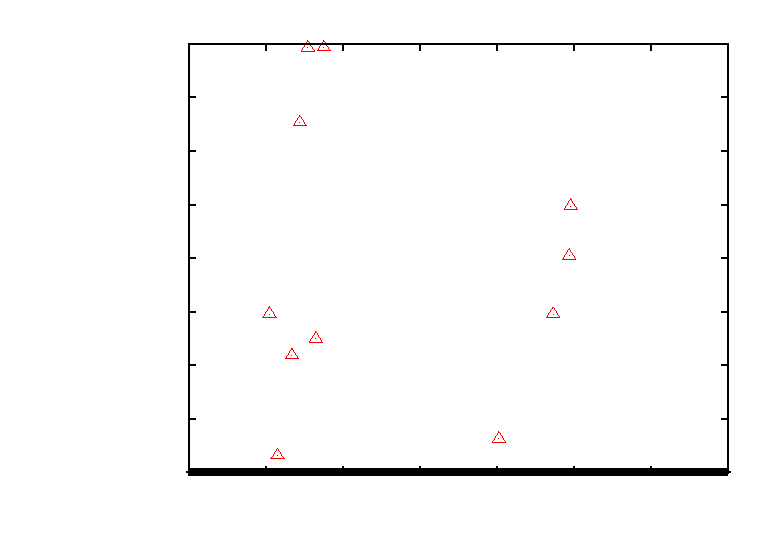
\includegraphics{fig/preempt1}}%
    \gplfronttext
  \end{picture}%
\endgroup
}}}\\
  \vspace{10pt}%
  \subfloat[][Os piores casos s�o representados no valor $15 \mu s$.]{%
    \label{fig:preempt2}%
    {\scalebox{1}{% GNUPLOT: LaTeX picture with Postscript
\begingroup
  \makeatletter
  \providecommand\color[2][]{%
    \GenericError{(gnuplot) \space\space\space\@spaces}{%
      Package color not loaded in conjunction with
      terminal option `colourtext'%
    }{See the gnuplot documentation for explanation.%
    }{Either use 'blacktext' in gnuplot or load the package
      color.sty in LaTeX.}%
    \renewcommand\color[2][]{}%
  }%
  \providecommand\includegraphics[2][]{%
    \GenericError{(gnuplot) \space\space\space\@spaces}{%
      Package graphicx or graphics not loaded%
    }{See the gnuplot documentation for explanation.%
    }{The gnuplot epslatex terminal needs graphicx.sty or graphics.sty.}%
    \renewcommand\includegraphics[2][]{}%
  }%
  \providecommand\rotatebox[2]{#2}%
  \@ifundefined{ifGPcolor}{%
    \newif\ifGPcolor
    \GPcolorfalse
  }{}%
  \@ifundefined{ifGPblacktext}{%
    \newif\ifGPblacktext
    \GPblacktextfalse
  }{}%
  % define a \g@addto@macro without @ in the name:
  \let\gplgaddtomacro\g@addto@macro
  % define empty templates for all commands taking text:
  \gdef\gplbacktext{}%
  \gdef\gplfronttext{}%
  \makeatother
  \ifGPblacktext
    % no textcolor at all
    \def\colorrgb#1{}%
    \def\colorgray#1{}%
  \else
    % gray or color?
    \ifGPcolor
      \def\colorrgb#1{\color[rgb]{#1}}%
      \def\colorgray#1{\color[gray]{#1}}%
      \expandafter\def\csname LTw\endcsname{\color{white}}%
      \expandafter\def\csname LTb\endcsname{\color{black}}%
      \expandafter\def\csname LTa\endcsname{\color{black}}%
      \expandafter\def\csname LT0\endcsname{\color[rgb]{1,0,0}}%
      \expandafter\def\csname LT1\endcsname{\color[rgb]{0,1,0}}%
      \expandafter\def\csname LT2\endcsname{\color[rgb]{0,0,1}}%
      \expandafter\def\csname LT3\endcsname{\color[rgb]{1,0,1}}%
      \expandafter\def\csname LT4\endcsname{\color[rgb]{0,1,1}}%
      \expandafter\def\csname LT5\endcsname{\color[rgb]{1,1,0}}%
      \expandafter\def\csname LT6\endcsname{\color[rgb]{0,0,0}}%
      \expandafter\def\csname LT7\endcsname{\color[rgb]{1,0.3,0}}%
      \expandafter\def\csname LT8\endcsname{\color[rgb]{0.5,0.5,0.5}}%
    \else
      % gray
      \def\colorrgb#1{\color{black}}%
      \def\colorgray#1{\color[gray]{#1}}%
      \expandafter\def\csname LTw\endcsname{\color{white}}%
      \expandafter\def\csname LTb\endcsname{\color{black}}%
      \expandafter\def\csname LTa\endcsname{\color{black}}%
      \expandafter\def\csname LT0\endcsname{\color{black}}%
      \expandafter\def\csname LT1\endcsname{\color{black}}%
      \expandafter\def\csname LT2\endcsname{\color{black}}%
      \expandafter\def\csname LT3\endcsname{\color{black}}%
      \expandafter\def\csname LT4\endcsname{\color{black}}%
      \expandafter\def\csname LT5\endcsname{\color{black}}%
      \expandafter\def\csname LT6\endcsname{\color{black}}%
      \expandafter\def\csname LT7\endcsname{\color{black}}%
      \expandafter\def\csname LT8\endcsname{\color{black}}%
    \fi
  \fi
  \setlength{\unitlength}{0.0500bp}%
  \begin{picture}(7200.00,5040.00)%
    \gplgaddtomacro\gplbacktext{%
      \csname LTb\endcsname%
      \put(1254,660){\makebox(0,0)[r]{\strut{}$8.0$}}%
      \put(1254,1175){\makebox(0,0)[r]{\strut{}$9.0$}}%
      \put(1254,1689){\makebox(0,0)[r]{\strut{}$10.0$}}%
      \put(1254,2204){\makebox(0,0)[r]{\strut{}$11.0$}}%
      \put(1254,2718){\makebox(0,0)[r]{\strut{}$12.0$}}%
      \put(1254,3233){\makebox(0,0)[r]{\strut{}$13.0$}}%
      \put(1254,3747){\makebox(0,0)[r]{\strut{}$14.0$}}%
      \put(1254,4262){\makebox(0,0)[r]{\strut{}$15.0$}}%
      \put(1254,4776){\makebox(0,0)[r]{\strut{}$16.0$}}%
      \put(1386,440){\makebox(0,0){\strut{}$ 0$}}%
      \put(2163,440){\makebox(0,0){\strut{}$ 10$}}%
      \put(2940,440){\makebox(0,0){\strut{}$ 20$}}%
      \put(3717,440){\makebox(0,0){\strut{}$ 30$}}%
      \put(4495,440){\makebox(0,0){\strut{}$ 40$}}%
      \put(5272,440){\makebox(0,0){\strut{}$ 50$}}%
      \put(6049,440){\makebox(0,0){\strut{}$ 60$}}%
      \put(6826,440){\makebox(0,0){\strut{}$ 70$}}%
      \put(220,2718){\rotatebox{90}{\makebox(0,0){\strut{}Lat\^encia em $\mu s$}}}%
      \put(4106,110){\makebox(0,0){\strut{}Tempo de execu\c{c}\~ao em $s$}}%
    }%
    \gplgaddtomacro\gplfronttext{%
    }%
    \gplbacktext
    \put(0,0){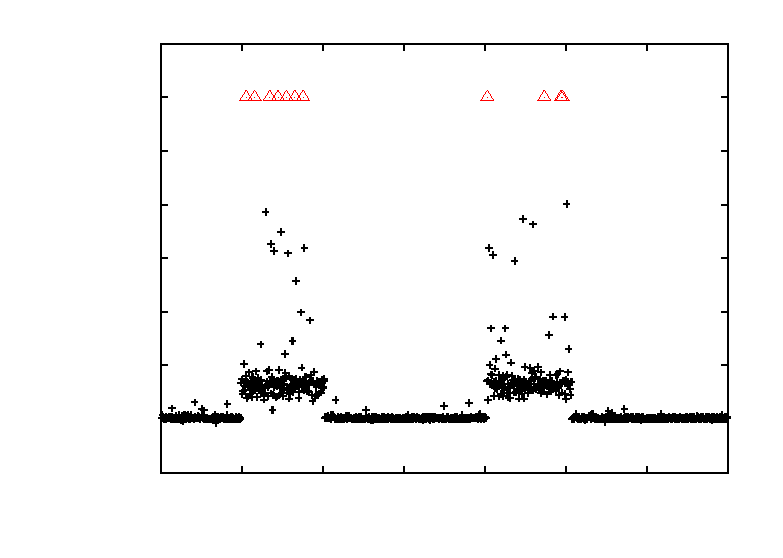
\includegraphics{fig/preempt2}}%
    \gplfronttext
  \end{picture}%
\endgroup
}}}%
  \caption[Lat�ncia de interrup��o de \preemptt]{Lat�ncia de interrup��o do
    \kernell Linux 2.6.23.9, com o \ing{patch} \preemptt. As figuras
    \subref{fig:preempt1} e \subref{fig:preempt2} representam a mesma execu��o.  A
    freq��ncia de interrup��o de $20 Hz$ e os dois estresses (60 aberturas e
    fechamento de sess�o \cod{ssh}) s�o aplicados nos instantes 10s e 40s.  Na
    figura \subref{fig:preempt2}, os piores casos s�o mostrados no valor $15 \mu s$
    para deixar os detalhes das demais medidas aparecer.}
  \label{fig:preempt}%
\end{figure}

A figura \ref{fig:klight} apresenta as lat�ncias de interrup��o observadas para o
\kernell Linux padr�o. Durante os dois per�odos de $10 s$ nos quais o estresse
\cod{ssh} � aplicado, os piores casos de lat�ncia, representados pelos tri�ngulos
vermelhos na figura \ref{fig:klight1}, chegam quase a $10 ms$.  No detalhe da figura
\ref{fig:klight2}, na qual os piores casos s�o representados no valor arbitr�rio de
$15 \mu s$, percebe-se que na aus�ncia de estresse, os tempos de lat�ncias s�o
bastante est�veis, abaixo de $10 \mu s$, em acordo com valores encontrados na
literatura \cite{Proctor01, Rostedt07, Siro07}. Durante a aplica��o dos estresses, a
lat�ncia da maioria dos eventos aumenta apenas de $1 \mu s$. Alguns eventos isolados
chegam a atingir at� 13 $\mu s$ de lat�ncia, enquanto, nos piores casos, a lat�ncia
atingi quase 1000 vezes o caso m�dio sem estresse.

Resultados similares foram obtidos com \preemptt como pode ser observado
nas figuras \ref{fig:preempt1} e \ref{fig:preempt2}. Esta semelhan�a era
de se esperar, j� que o c�digo da camada de rede do Linux � bastante otimizado, e que,
conseq�entemente, as melhorias trazidas por \preemptt n�o afetam as caracter�sticas 
temporal desta camada.

No caso do Linux, $6$ eventos tiveram uma lat�ncia superior a $20 \mu s$ e no
\preemptt foram 11 eventos similares observados.  Portanto, apesar da maioria dos
eventos - mais de 400 ao total nos dois per�odos de estresse - n�o sofrer lat�ncia
superior a $14 \mu s$, pode-se concluir que a exist�ncia de lat�ncias de quase $10ms$
nos piores casos observados inviabilizam a utiliza��o destas duas plataformas no
contexto de sistema de tempo real cr�tico.


\subsubsection{RTAI e Xenomai}

Para os experimentos com RTAI e Xenomai, foi mencionado na se��o \ref{sec:dispExp}
que a transfer�ncia dos dados da mem�ria do \kernell para o sistema de arquivo foi
realizada com os canais \ing{RT-FIFO} proporcionados pela API destas duas
plataformas. Apesar das garantias ofertas pela implementa��o destas plataformas,
considerou-se a possibilidade que o acesso ass�ncrono aos canais \cod{RT-FIFO} por
um processo usu�rio poderia interferir nas medidas. Portanto, realizou-se os
experimentos com duas configura��es diferentes. Na primeira, os canais foram
consultados entre cada escrita na porta paralela e na segunda, o acesso s� aconteceu
a cada 20 escrita na porta paralela.  Em ambos os casos, a freq��ncia de escrita na
porta paralela era de $20 Hz$.

Os resultados destes dois modos de opera��o s�o apresentados nas figuras
\ref{fig:rtai} para RTAI e \ref{fig:xeno} para Xenomai. Constata-se que os eventos
extremos s�o mais raros e tem valores menores que no caso do Linux e do
\preempt. Com RTAI, observou-se um evento extremo de $165 \mu s$ na primeira
configura��o do experimento. Nos dois outros modos, um evento extremo isolado tamb�m
aconteceu, com a mesma ordem de grandeza.

Com o Xenomai, v�rios experimentos repetidos na primeira configura��o n�o permitiram
de observar evento extremo algum. No entanto, com o segundo modo experimental, no
qual a leitura do canal \cod{RT-FIFO} foi realizada com uma freq��ncia menor,
piores casos da mesma ordem de grandeza que no RTAI foram observados.

\begin{figure}%
  \centering
  \subfloat[O tri�ngulo vermelho corresponde a um pior caso isolado (de $165.3 \mu s$)]{%
    \label{fig:rtai2}%
    {\scalebox{1}{% GNUPLOT: LaTeX picture with Postscript
\begingroup
  \makeatletter
  \providecommand\color[2][]{%
    \GenericError{(gnuplot) \space\space\space\@spaces}{%
      Package color not loaded in conjunction with
      terminal option `colourtext'%
    }{See the gnuplot documentation for explanation.%
    }{Either use 'blacktext' in gnuplot or load the package
      color.sty in LaTeX.}%
    \renewcommand\color[2][]{}%
  }%
  \providecommand\includegraphics[2][]{%
    \GenericError{(gnuplot) \space\space\space\@spaces}{%
      Package graphicx or graphics not loaded%
    }{See the gnuplot documentation for explanation.%
    }{The gnuplot epslatex terminal needs graphicx.sty or graphics.sty.}%
    \renewcommand\includegraphics[2][]{}%
  }%
  \providecommand\rotatebox[2]{#2}%
  \@ifundefined{ifGPcolor}{%
    \newif\ifGPcolor
    \GPcolorfalse
  }{}%
  \@ifundefined{ifGPblacktext}{%
    \newif\ifGPblacktext
    \GPblacktextfalse
  }{}%
  % define a \g@addto@macro without @ in the name:
  \let\gplgaddtomacro\g@addto@macro
  % define empty templates for all commands taking text:
  \gdef\gplbacktext{}%
  \gdef\gplfronttext{}%
  \makeatother
  \ifGPblacktext
    % no textcolor at all
    \def\colorrgb#1{}%
    \def\colorgray#1{}%
  \else
    % gray or color?
    \ifGPcolor
      \def\colorrgb#1{\color[rgb]{#1}}%
      \def\colorgray#1{\color[gray]{#1}}%
      \expandafter\def\csname LTw\endcsname{\color{white}}%
      \expandafter\def\csname LTb\endcsname{\color{black}}%
      \expandafter\def\csname LTa\endcsname{\color{black}}%
      \expandafter\def\csname LT0\endcsname{\color[rgb]{1,0,0}}%
      \expandafter\def\csname LT1\endcsname{\color[rgb]{0,1,0}}%
      \expandafter\def\csname LT2\endcsname{\color[rgb]{0,0,1}}%
      \expandafter\def\csname LT3\endcsname{\color[rgb]{1,0,1}}%
      \expandafter\def\csname LT4\endcsname{\color[rgb]{0,1,1}}%
      \expandafter\def\csname LT5\endcsname{\color[rgb]{1,1,0}}%
      \expandafter\def\csname LT6\endcsname{\color[rgb]{0,0,0}}%
      \expandafter\def\csname LT7\endcsname{\color[rgb]{1,0.3,0}}%
      \expandafter\def\csname LT8\endcsname{\color[rgb]{0.5,0.5,0.5}}%
    \else
      % gray
      \def\colorrgb#1{\color{black}}%
      \def\colorgray#1{\color[gray]{#1}}%
      \expandafter\def\csname LTw\endcsname{\color{white}}%
      \expandafter\def\csname LTb\endcsname{\color{black}}%
      \expandafter\def\csname LTa\endcsname{\color{black}}%
      \expandafter\def\csname LT0\endcsname{\color{black}}%
      \expandafter\def\csname LT1\endcsname{\color{black}}%
      \expandafter\def\csname LT2\endcsname{\color{black}}%
      \expandafter\def\csname LT3\endcsname{\color{black}}%
      \expandafter\def\csname LT4\endcsname{\color{black}}%
      \expandafter\def\csname LT5\endcsname{\color{black}}%
      \expandafter\def\csname LT6\endcsname{\color{black}}%
      \expandafter\def\csname LT7\endcsname{\color{black}}%
      \expandafter\def\csname LT8\endcsname{\color{black}}%
    \fi
  \fi
  \setlength{\unitlength}{0.0500bp}%
  \begin{picture}(7200.00,5040.00)%
    \gplgaddtomacro\gplbacktext{%
      \csname LTb\endcsname%
      \put(1254,660){\makebox(0,0)[r]{\strut{}$9.0$}}%
      \put(1254,1248){\makebox(0,0)[r]{\strut{}$10.0$}}%
      \put(1254,1836){\makebox(0,0)[r]{\strut{}$11.0$}}%
      \put(1254,2424){\makebox(0,0)[r]{\strut{}$12.0$}}%
      \put(1254,3012){\makebox(0,0)[r]{\strut{}$13.0$}}%
      \put(1254,3600){\makebox(0,0)[r]{\strut{}$14.0$}}%
      \put(1254,4188){\makebox(0,0)[r]{\strut{}$15.0$}}%
      \put(1254,4776){\makebox(0,0)[r]{\strut{}$16.0$}}%
      \put(1386,440){\makebox(0,0){\strut{}$ 0$}}%
      \put(2163,440){\makebox(0,0){\strut{}$ 10$}}%
      \put(2940,440){\makebox(0,0){\strut{}$ 20$}}%
      \put(3717,440){\makebox(0,0){\strut{}$ 30$}}%
      \put(4495,440){\makebox(0,0){\strut{}$ 40$}}%
      \put(5272,440){\makebox(0,0){\strut{}$ 50$}}%
      \put(6049,440){\makebox(0,0){\strut{}$ 60$}}%
      \put(6826,440){\makebox(0,0){\strut{}$ 70$}}%
      \put(220,2718){\rotatebox{90}{\makebox(0,0){\strut{}Lat\^encia em $\mu s$}}}%
      \put(4106,110){\makebox(0,0){\strut{}Tempo de execu\c{c}\~ao em $s$}}%
      \put(4339,4364){\makebox(0,0)[l]{\strut{}165.3}}%
    }%
    \gplgaddtomacro\gplfronttext{%
    }%
    \gplbacktext
    \put(0,0){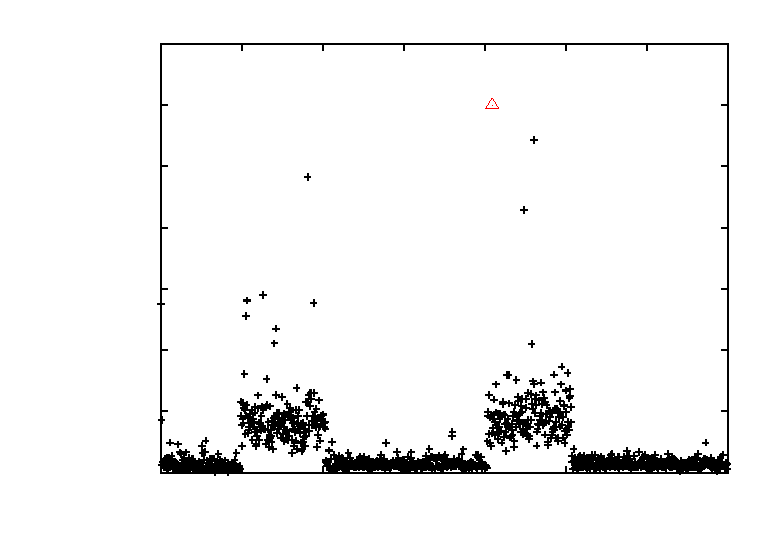
\includegraphics{fig/rtai2}}%
    \gplfronttext
  \end{picture}%
\endgroup
}}}\\
  \vspace{10pt}%
  \subfloat[][M�dia sobre 20 eventos.]{%
    \label{fig:rtaiM2}%
    {\scalebox{1}{% GNUPLOT: LaTeX picture with Postscript
\begingroup
  \makeatletter
  \providecommand\color[2][]{%
    \GenericError{(gnuplot) \space\space\space\@spaces}{%
      Package color not loaded in conjunction with
      terminal option `colourtext'%
    }{See the gnuplot documentation for explanation.%
    }{Either use 'blacktext' in gnuplot or load the package
      color.sty in LaTeX.}%
    \renewcommand\color[2][]{}%
  }%
  \providecommand\includegraphics[2][]{%
    \GenericError{(gnuplot) \space\space\space\@spaces}{%
      Package graphicx or graphics not loaded%
    }{See the gnuplot documentation for explanation.%
    }{The gnuplot epslatex terminal needs graphicx.sty or graphics.sty.}%
    \renewcommand\includegraphics[2][]{}%
  }%
  \providecommand\rotatebox[2]{#2}%
  \@ifundefined{ifGPcolor}{%
    \newif\ifGPcolor
    \GPcolorfalse
  }{}%
  \@ifundefined{ifGPblacktext}{%
    \newif\ifGPblacktext
    \GPblacktextfalse
  }{}%
  % define a \g@addto@macro without @ in the name:
  \let\gplgaddtomacro\g@addto@macro
  % define empty templates for all commands taking text:
  \gdef\gplbacktext{}%
  \gdef\gplfronttext{}%
  \makeatother
  \ifGPblacktext
    % no textcolor at all
    \def\colorrgb#1{}%
    \def\colorgray#1{}%
  \else
    % gray or color?
    \ifGPcolor
      \def\colorrgb#1{\color[rgb]{#1}}%
      \def\colorgray#1{\color[gray]{#1}}%
      \expandafter\def\csname LTw\endcsname{\color{white}}%
      \expandafter\def\csname LTb\endcsname{\color{black}}%
      \expandafter\def\csname LTa\endcsname{\color{black}}%
      \expandafter\def\csname LT0\endcsname{\color[rgb]{1,0,0}}%
      \expandafter\def\csname LT1\endcsname{\color[rgb]{0,1,0}}%
      \expandafter\def\csname LT2\endcsname{\color[rgb]{0,0,1}}%
      \expandafter\def\csname LT3\endcsname{\color[rgb]{1,0,1}}%
      \expandafter\def\csname LT4\endcsname{\color[rgb]{0,1,1}}%
      \expandafter\def\csname LT5\endcsname{\color[rgb]{1,1,0}}%
      \expandafter\def\csname LT6\endcsname{\color[rgb]{0,0,0}}%
      \expandafter\def\csname LT7\endcsname{\color[rgb]{1,0.3,0}}%
      \expandafter\def\csname LT8\endcsname{\color[rgb]{0.5,0.5,0.5}}%
    \else
      % gray
      \def\colorrgb#1{\color{black}}%
      \def\colorgray#1{\color[gray]{#1}}%
      \expandafter\def\csname LTw\endcsname{\color{white}}%
      \expandafter\def\csname LTb\endcsname{\color{black}}%
      \expandafter\def\csname LTa\endcsname{\color{black}}%
      \expandafter\def\csname LT0\endcsname{\color{black}}%
      \expandafter\def\csname LT1\endcsname{\color{black}}%
      \expandafter\def\csname LT2\endcsname{\color{black}}%
      \expandafter\def\csname LT3\endcsname{\color{black}}%
      \expandafter\def\csname LT4\endcsname{\color{black}}%
      \expandafter\def\csname LT5\endcsname{\color{black}}%
      \expandafter\def\csname LT6\endcsname{\color{black}}%
      \expandafter\def\csname LT7\endcsname{\color{black}}%
      \expandafter\def\csname LT8\endcsname{\color{black}}%
    \fi
  \fi
  \setlength{\unitlength}{0.0500bp}%
  \begin{picture}(7200.00,5040.00)%
    \gplgaddtomacro\gplbacktext{%
      \csname LTb\endcsname%
      \put(1254,660){\makebox(0,0)[r]{\strut{}$9.0$}}%
      \put(1254,1117){\makebox(0,0)[r]{\strut{}$10.0$}}%
      \put(1254,1575){\makebox(0,0)[r]{\strut{}$11.0$}}%
      \put(1254,2032){\makebox(0,0)[r]{\strut{}$12.0$}}%
      \put(1254,2489){\makebox(0,0)[r]{\strut{}$13.0$}}%
      \put(1254,2947){\makebox(0,0)[r]{\strut{}$14.0$}}%
      \put(1254,3404){\makebox(0,0)[r]{\strut{}$15.0$}}%
      \put(1254,3861){\makebox(0,0)[r]{\strut{}$16.0$}}%
      \put(1254,4319){\makebox(0,0)[r]{\strut{}$17.0$}}%
      \put(1254,4776){\makebox(0,0)[r]{\strut{}$18.0$}}%
      \put(1386,440){\makebox(0,0){\strut{}$ 0$}}%
      \put(2163,440){\makebox(0,0){\strut{}$ 10$}}%
      \put(2940,440){\makebox(0,0){\strut{}$ 20$}}%
      \put(3717,440){\makebox(0,0){\strut{}$ 30$}}%
      \put(4495,440){\makebox(0,0){\strut{}$ 40$}}%
      \put(5272,440){\makebox(0,0){\strut{}$ 50$}}%
      \put(6049,440){\makebox(0,0){\strut{}$ 60$}}%
      \put(6826,440){\makebox(0,0){\strut{}$ 70$}}%
      \put(220,2718){\rotatebox{90}{\makebox(0,0){\strut{}Lat\^encia em $\mu s$}}}%
      \put(4106,110){\makebox(0,0){\strut{}Tempo de execu\c{c}\~ao em $s$}}%
      \put(4883,4319){\makebox(0,0)[l]{\strut{}Desvio padr\~ao}}%
      \put(4883,4099){\makebox(0,0)[l]{\strut{}m\'{a}ximo 44.0}}%
    }%
    \gplgaddtomacro\gplfronttext{%
    }%
    \gplbacktext
    \put(0,0){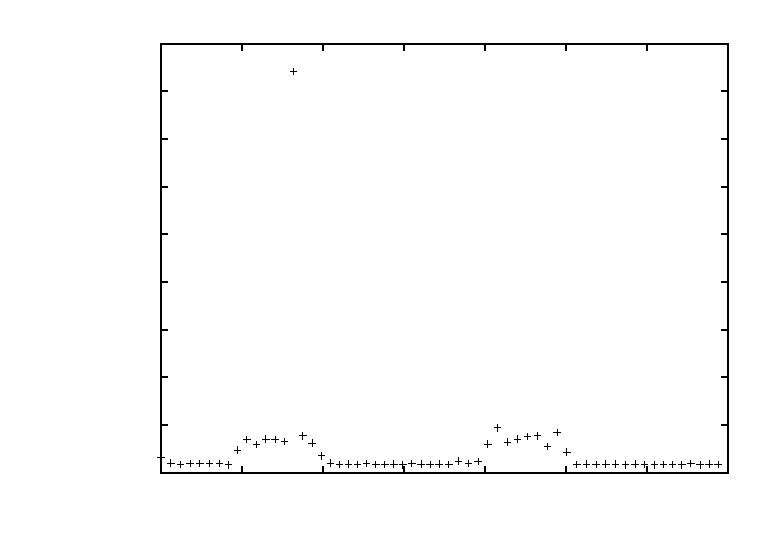
\includegraphics{fig/rtaiM2}}%
    \gplfronttext
  \end{picture}%
\endgroup
}}}%
  \caption[Lat�ncia de interrup��o do RTAI]{Lat�ncia de interrup��o do \kernell
    Linux 2.6.19.7, com o \ing{patch} RTAI ``magma''. As figuras \subref{fig:rtai2}
    e \subref{fig:rtaiM2} representam execu��es na freq��ncia de interrup��o de $20
    Hz$. Os dois estresses (60 aberturas e fechamento de sess�o \cod{ssh}) s�o
    aplicados nos instantes 10s e 40s.  Na figura \subref{fig:rtai2}, o pior caso �
    mostrado no valor $15 \mu s$ para deixar os detalhes das demais medidas
    aparecer. Na figura \subref{fig:rtaiM2}, o canal RT-FIFO � consultado a cada 20
    interrup��es e a m�dia correspondente � calculada.}
  \label{fig:rtai}%
\end{figure}

\begin{figure}%
  \centering
  \subfloat[Valores instant�neos.]{%
    \label{fig:xeno1}%
    {\scalebox{1}{% GNUPLOT: LaTeX picture with Postscript
\begingroup
  \makeatletter
  \providecommand\color[2][]{%
    \GenericError{(gnuplot) \space\space\space\@spaces}{%
      Package color not loaded in conjunction with
      terminal option `colourtext'%
    }{See the gnuplot documentation for explanation.%
    }{Either use 'blacktext' in gnuplot or load the package
      color.sty in LaTeX.}%
    \renewcommand\color[2][]{}%
  }%
  \providecommand\includegraphics[2][]{%
    \GenericError{(gnuplot) \space\space\space\@spaces}{%
      Package graphicx or graphics not loaded%
    }{See the gnuplot documentation for explanation.%
    }{The gnuplot epslatex terminal needs graphicx.sty or graphics.sty.}%
    \renewcommand\includegraphics[2][]{}%
  }%
  \providecommand\rotatebox[2]{#2}%
  \@ifundefined{ifGPcolor}{%
    \newif\ifGPcolor
    \GPcolorfalse
  }{}%
  \@ifundefined{ifGPblacktext}{%
    \newif\ifGPblacktext
    \GPblacktextfalse
  }{}%
  % define a \g@addto@macro without @ in the name:
  \let\gplgaddtomacro\g@addto@macro
  % define empty templates for all commands taking text:
  \gdef\gplbacktext{}%
  \gdef\gplfronttext{}%
  \makeatother
  \ifGPblacktext
    % no textcolor at all
    \def\colorrgb#1{}%
    \def\colorgray#1{}%
  \else
    % gray or color?
    \ifGPcolor
      \def\colorrgb#1{\color[rgb]{#1}}%
      \def\colorgray#1{\color[gray]{#1}}%
      \expandafter\def\csname LTw\endcsname{\color{white}}%
      \expandafter\def\csname LTb\endcsname{\color{black}}%
      \expandafter\def\csname LTa\endcsname{\color{black}}%
      \expandafter\def\csname LT0\endcsname{\color[rgb]{1,0,0}}%
      \expandafter\def\csname LT1\endcsname{\color[rgb]{0,1,0}}%
      \expandafter\def\csname LT2\endcsname{\color[rgb]{0,0,1}}%
      \expandafter\def\csname LT3\endcsname{\color[rgb]{1,0,1}}%
      \expandafter\def\csname LT4\endcsname{\color[rgb]{0,1,1}}%
      \expandafter\def\csname LT5\endcsname{\color[rgb]{1,1,0}}%
      \expandafter\def\csname LT6\endcsname{\color[rgb]{0,0,0}}%
      \expandafter\def\csname LT7\endcsname{\color[rgb]{1,0.3,0}}%
      \expandafter\def\csname LT8\endcsname{\color[rgb]{0.5,0.5,0.5}}%
    \else
      % gray
      \def\colorrgb#1{\color{black}}%
      \def\colorgray#1{\color[gray]{#1}}%
      \expandafter\def\csname LTw\endcsname{\color{white}}%
      \expandafter\def\csname LTb\endcsname{\color{black}}%
      \expandafter\def\csname LTa\endcsname{\color{black}}%
      \expandafter\def\csname LT0\endcsname{\color{black}}%
      \expandafter\def\csname LT1\endcsname{\color{black}}%
      \expandafter\def\csname LT2\endcsname{\color{black}}%
      \expandafter\def\csname LT3\endcsname{\color{black}}%
      \expandafter\def\csname LT4\endcsname{\color{black}}%
      \expandafter\def\csname LT5\endcsname{\color{black}}%
      \expandafter\def\csname LT6\endcsname{\color{black}}%
      \expandafter\def\csname LT7\endcsname{\color{black}}%
      \expandafter\def\csname LT8\endcsname{\color{black}}%
    \fi
  \fi
  \setlength{\unitlength}{0.0500bp}%
  \begin{picture}(7200.00,5040.00)%
    \gplgaddtomacro\gplbacktext{%
      \csname LTb\endcsname%
      \put(1254,660){\makebox(0,0)[r]{\strut{}$9.0$}}%
      \put(1254,1346){\makebox(0,0)[r]{\strut{}$10.0$}}%
      \put(1254,2032){\makebox(0,0)[r]{\strut{}$11.0$}}%
      \put(1254,2718){\makebox(0,0)[r]{\strut{}$12.0$}}%
      \put(1254,3404){\makebox(0,0)[r]{\strut{}$13.0$}}%
      \put(1254,4090){\makebox(0,0)[r]{\strut{}$14.0$}}%
      \put(1254,4776){\makebox(0,0)[r]{\strut{}$15.0$}}%
      \put(1386,440){\makebox(0,0){\strut{}$ 0$}}%
      \put(2163,440){\makebox(0,0){\strut{}$ 10$}}%
      \put(2940,440){\makebox(0,0){\strut{}$ 20$}}%
      \put(3717,440){\makebox(0,0){\strut{}$ 30$}}%
      \put(4495,440){\makebox(0,0){\strut{}$ 40$}}%
      \put(5272,440){\makebox(0,0){\strut{}$ 50$}}%
      \put(6049,440){\makebox(0,0){\strut{}$ 60$}}%
      \put(6826,440){\makebox(0,0){\strut{}$ 70$}}%
      \put(220,2718){\rotatebox{90}{\makebox(0,0){\strut{}Lat\^encia em $\mu s$}}}%
      \put(4106,110){\makebox(0,0){\strut{}Tempo de execu\c{c}\~ao em $s$}}%
    }%
    \gplgaddtomacro\gplfronttext{%
    }%
    \gplbacktext
    \put(0,0){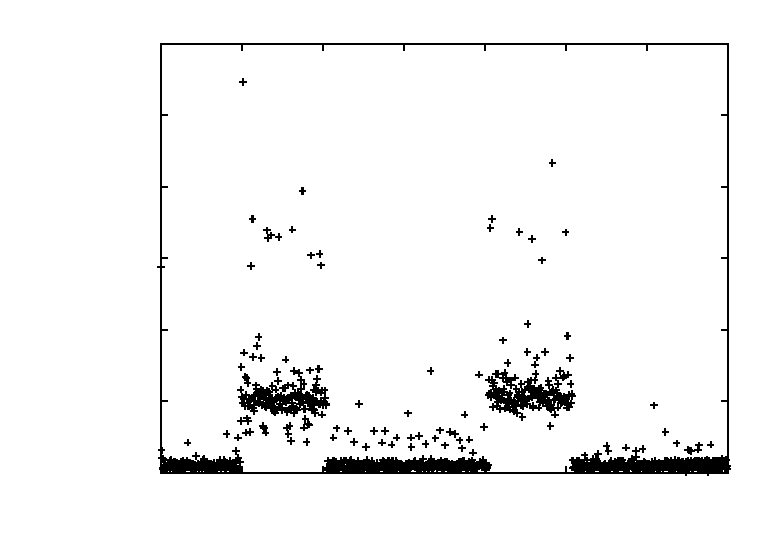
\includegraphics{fig/xeno1}}%
    \gplfronttext
  \end{picture}%
\endgroup
}}}\\
  \vspace{10pt}%
  \subfloat[][M�dia sobre 20 eventos.]{%
    \label{fig:xenoM1}%
    {\scalebox{1}{% GNUPLOT: LaTeX picture with Postscript
\begingroup
  \makeatletter
  \providecommand\color[2][]{%
    \GenericError{(gnuplot) \space\space\space\@spaces}{%
      Package color not loaded in conjunction with
      terminal option `colourtext'%
    }{See the gnuplot documentation for explanation.%
    }{Either use 'blacktext' in gnuplot or load the package
      color.sty in LaTeX.}%
    \renewcommand\color[2][]{}%
  }%
  \providecommand\includegraphics[2][]{%
    \GenericError{(gnuplot) \space\space\space\@spaces}{%
      Package graphicx or graphics not loaded%
    }{See the gnuplot documentation for explanation.%
    }{The gnuplot epslatex terminal needs graphicx.sty or graphics.sty.}%
    \renewcommand\includegraphics[2][]{}%
  }%
  \providecommand\rotatebox[2]{#2}%
  \@ifundefined{ifGPcolor}{%
    \newif\ifGPcolor
    \GPcolorfalse
  }{}%
  \@ifundefined{ifGPblacktext}{%
    \newif\ifGPblacktext
    \GPblacktextfalse
  }{}%
  % define a \g@addto@macro without @ in the name:
  \let\gplgaddtomacro\g@addto@macro
  % define empty templates for all commands taking text:
  \gdef\gplbacktext{}%
  \gdef\gplfronttext{}%
  \makeatother
  \ifGPblacktext
    % no textcolor at all
    \def\colorrgb#1{}%
    \def\colorgray#1{}%
  \else
    % gray or color?
    \ifGPcolor
      \def\colorrgb#1{\color[rgb]{#1}}%
      \def\colorgray#1{\color[gray]{#1}}%
      \expandafter\def\csname LTw\endcsname{\color{white}}%
      \expandafter\def\csname LTb\endcsname{\color{black}}%
      \expandafter\def\csname LTa\endcsname{\color{black}}%
      \expandafter\def\csname LT0\endcsname{\color[rgb]{1,0,0}}%
      \expandafter\def\csname LT1\endcsname{\color[rgb]{0,1,0}}%
      \expandafter\def\csname LT2\endcsname{\color[rgb]{0,0,1}}%
      \expandafter\def\csname LT3\endcsname{\color[rgb]{1,0,1}}%
      \expandafter\def\csname LT4\endcsname{\color[rgb]{0,1,1}}%
      \expandafter\def\csname LT5\endcsname{\color[rgb]{1,1,0}}%
      \expandafter\def\csname LT6\endcsname{\color[rgb]{0,0,0}}%
      \expandafter\def\csname LT7\endcsname{\color[rgb]{1,0.3,0}}%
      \expandafter\def\csname LT8\endcsname{\color[rgb]{0.5,0.5,0.5}}%
    \else
      % gray
      \def\colorrgb#1{\color{black}}%
      \def\colorgray#1{\color[gray]{#1}}%
      \expandafter\def\csname LTw\endcsname{\color{white}}%
      \expandafter\def\csname LTb\endcsname{\color{black}}%
      \expandafter\def\csname LTa\endcsname{\color{black}}%
      \expandafter\def\csname LT0\endcsname{\color{black}}%
      \expandafter\def\csname LT1\endcsname{\color{black}}%
      \expandafter\def\csname LT2\endcsname{\color{black}}%
      \expandafter\def\csname LT3\endcsname{\color{black}}%
      \expandafter\def\csname LT4\endcsname{\color{black}}%
      \expandafter\def\csname LT5\endcsname{\color{black}}%
      \expandafter\def\csname LT6\endcsname{\color{black}}%
      \expandafter\def\csname LT7\endcsname{\color{black}}%
      \expandafter\def\csname LT8\endcsname{\color{black}}%
    \fi
  \fi
  \setlength{\unitlength}{0.0500bp}%
  \begin{picture}(7200.00,5040.00)%
    \gplgaddtomacro\gplbacktext{%
      \csname LTb\endcsname%
      \put(1254,660){\makebox(0,0)[r]{\strut{}$9.0$}}%
      \put(1254,1072){\makebox(0,0)[r]{\strut{}$10.0$}}%
      \put(1254,1483){\makebox(0,0)[r]{\strut{}$11.0$}}%
      \put(1254,1895){\makebox(0,0)[r]{\strut{}$12.0$}}%
      \put(1254,2306){\makebox(0,0)[r]{\strut{}$13.0$}}%
      \put(1254,2718){\makebox(0,0)[r]{\strut{}$14.0$}}%
      \put(1254,3130){\makebox(0,0)[r]{\strut{}$15.0$}}%
      \put(1254,3541){\makebox(0,0)[r]{\strut{}$16.0$}}%
      \put(1254,3953){\makebox(0,0)[r]{\strut{}$17.0$}}%
      \put(1254,4364){\makebox(0,0)[r]{\strut{}$18.0$}}%
      \put(1254,4776){\makebox(0,0)[r]{\strut{}$19.0$}}%
      \put(1386,440){\makebox(0,0){\strut{}$ 0$}}%
      \put(2163,440){\makebox(0,0){\strut{}$ 10$}}%
      \put(2940,440){\makebox(0,0){\strut{}$ 20$}}%
      \put(3717,440){\makebox(0,0){\strut{}$ 30$}}%
      \put(4495,440){\makebox(0,0){\strut{}$ 40$}}%
      \put(5272,440){\makebox(0,0){\strut{}$ 50$}}%
      \put(6049,440){\makebox(0,0){\strut{}$ 60$}}%
      \put(6826,440){\makebox(0,0){\strut{}$ 70$}}%
      \put(220,2718){\rotatebox{90}{\makebox(0,0){\strut{}Lat\^encia em $\mu s$}}}%
      \put(4106,110){\makebox(0,0){\strut{}Tempo de execu\c{c}\~ao em $s$}}%
      \put(5116,4364){\makebox(0,0)[l]{\strut{}Desvio padr\~ao}}%
      \put(5116,4144){\makebox(0,0)[l]{\strut{}m\'{a}ximo 34.1}}%
    }%
    \gplgaddtomacro\gplfronttext{%
    }%
    \gplbacktext
    \put(0,0){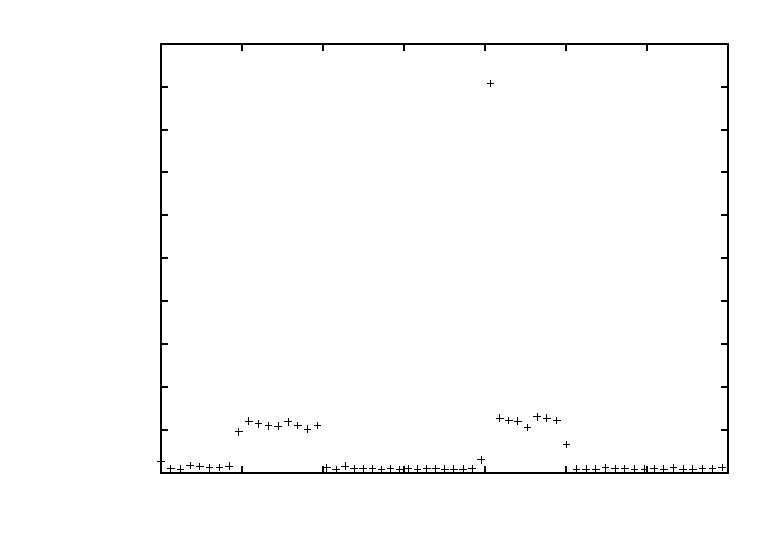
\includegraphics{fig/xenoM1}}%
    \gplfronttext
  \end{picture}%
\endgroup
}}}%
  \caption[Lat�ncia de interrup��o do Xenomai]{Lat�ncia de interrup��o do \kernell
    Linux 2.6.19.7, com o \ing{patch} Xenomai 2.4-rc5. As figuras \subref{fig:xeno1}
    e \subref{fig:xenoM1} representam execu��es na freq��ncia de interrup��o de $20
    Hz$. Os dois estresses (60 aberturas e fechamento de sess�o \cod{ssh}) s�o
    aplicados nos instantes 10s e 40s. Na figura \subref{fig:xenoM1}, o canal
    RT-FIFO � consultado a cada 20 interrup��es e a m�dia correspondente �
    calculada.}
  \label{fig:xeno}%
\end{figure}

Em conclus�o destes experimentos, considerou-se que as plataformas Linux e \preemptt
n�o podiam dar as garantias temporais necess�rias para a implementa��o do protocolo
\doris. Apesar de n�o constituir um conjunto suficiente de avalia��o, os resultados
com as plataformas RTAI e Xenomai mostraram que estas plataformas tem um
comportamento similares em que diz respeito a lat�ncia de interrup��o e que elas s�o
mais determin�sticas que Linux e \preempt. As ocorr�ncias de valores de lat�ncias
altas n�o ultrapassaram $200 \mu s$ e aconteceram numa freq��ncia m�xima 
de uma vez em 400 eventos. Do ponto de visto da implementa��o do protocolo 
\doris, estes resultados confirmaram o ganho significativo de se trabalhar com 
as plataformas RTAI e Xenomai. No entanto, a exist�ncia de piores casos 
demonstra a necessidade de utilizar mecanismo de toler�ncia para 
manter as garantias do protocolo de comunica��o, apesar destes eventos isolados.

Observa-se tamb�m que os experimentos foram realizadas numa
arquitetura especifica e que resultados quantitativamente diferentes teriam
provavelmente sido encontradas em outras configura��es de m�quinas. No entanto,
os resultados obtidos aqui s�o qualitativamente consistente com os resultados
apresentados em trabalhos similares \cite{McKenney05, Siro07, Dozio03}.

Al�m das medidas de interrup��o, medidas de lat�ncias de escalonamento e de tempos
de execu��o s�o mostradas nas figuras \ref{fig:latEscal}. Estas medidas foram
realizadas com a metodologia descrita na se��o \label{sec:dispExp}. A lat�ncia de
escalonamento corresponde ao tempo que passa entre a execu��o do tratador de
interrup��o e o instante no qual a tarefa $T$ suspensa come�a a executar. O tempo de
execu��o corresponde ao tempo do qual $T$ precisa para criar um pacote Ethernet de
64 bytes e transferi-lo para a placa de rede. Na aus�ncia de estresse, observa-se na
figura \ref{fig:latEscal} que estes tempos s�o est�vel em ambas plataformas. No caso
do RTAI, observa-se que a lat�ncia de escalonamento � da ordem de $1 \mu s$,
enquanto para Xenomai, ela � da ordem de $4 \mu s$.  Esta diferen�a se deve aos
modelos de tarefas diferentes nestas duas plataformas. Como foi visto na se��o
\ref{sec:adeos}, Xenomai privilegia a integra��o com o modo usu�rio do Linux e uma
das conseq��ncias deste modelo de desenvolvimento � a exist�ncia de uma sobrecarga
na troca de contexto de uma tarefa \cite{Gerum05}.

\begin{figure}%
  \centering
  \subfloat[Lat�ncias do RTAI]{%
    \label{fig:rtaiEsc}%
    {\scalebox{0.9}{% GNUPLOT: LaTeX picture with Postscript
\begingroup
  \makeatletter
  \providecommand\color[2][]{%
    \GenericError{(gnuplot) \space\space\space\@spaces}{%
      Package color not loaded in conjunction with
      terminal option `colourtext'%
    }{See the gnuplot documentation for explanation.%
    }{Either use 'blacktext' in gnuplot or load the package
      color.sty in LaTeX.}%
    \renewcommand\color[2][]{}%
  }%
  \providecommand\includegraphics[2][]{%
    \GenericError{(gnuplot) \space\space\space\@spaces}{%
      Package graphicx or graphics not loaded%
    }{See the gnuplot documentation for explanation.%
    }{The gnuplot epslatex terminal needs graphicx.sty or graphics.sty.}%
    \renewcommand\includegraphics[2][]{}%
  }%
  \providecommand\rotatebox[2]{#2}%
  \@ifundefined{ifGPcolor}{%
    \newif\ifGPcolor
    \GPcolorfalse
  }{}%
  \@ifundefined{ifGPblacktext}{%
    \newif\ifGPblacktext
    \GPblacktextfalse
  }{}%
  % define a \g@addto@macro without @ in the name:
  \let\gplgaddtomacro\g@addto@macro
  % define empty templates for all commands taking text:
  \gdef\gplbacktext{}%
  \gdef\gplfronttext{}%
  \makeatother
  \ifGPblacktext
    % no textcolor at all
    \def\colorrgb#1{}%
    \def\colorgray#1{}%
  \else
    % gray or color?
    \ifGPcolor
      \def\colorrgb#1{\color[rgb]{#1}}%
      \def\colorgray#1{\color[gray]{#1}}%
      \expandafter\def\csname LTw\endcsname{\color{white}}%
      \expandafter\def\csname LTb\endcsname{\color{black}}%
      \expandafter\def\csname LTa\endcsname{\color{black}}%
      \expandafter\def\csname LT0\endcsname{\color[rgb]{1,0,0}}%
      \expandafter\def\csname LT1\endcsname{\color[rgb]{0,1,0}}%
      \expandafter\def\csname LT2\endcsname{\color[rgb]{0,0,1}}%
      \expandafter\def\csname LT3\endcsname{\color[rgb]{1,0,1}}%
      \expandafter\def\csname LT4\endcsname{\color[rgb]{0,1,1}}%
      \expandafter\def\csname LT5\endcsname{\color[rgb]{1,1,0}}%
      \expandafter\def\csname LT6\endcsname{\color[rgb]{0,0,0}}%
      \expandafter\def\csname LT7\endcsname{\color[rgb]{1,0.3,0}}%
      \expandafter\def\csname LT8\endcsname{\color[rgb]{0.5,0.5,0.5}}%
    \else
      % gray
      \def\colorrgb#1{\color{black}}%
      \def\colorgray#1{\color[gray]{#1}}%
      \expandafter\def\csname LTw\endcsname{\color{white}}%
      \expandafter\def\csname LTb\endcsname{\color{black}}%
      \expandafter\def\csname LTa\endcsname{\color{black}}%
      \expandafter\def\csname LT0\endcsname{\color{black}}%
      \expandafter\def\csname LT1\endcsname{\color{black}}%
      \expandafter\def\csname LT2\endcsname{\color{black}}%
      \expandafter\def\csname LT3\endcsname{\color{black}}%
      \expandafter\def\csname LT4\endcsname{\color{black}}%
      \expandafter\def\csname LT5\endcsname{\color{black}}%
      \expandafter\def\csname LT6\endcsname{\color{black}}%
      \expandafter\def\csname LT7\endcsname{\color{black}}%
      \expandafter\def\csname LT8\endcsname{\color{black}}%
    \fi
  \fi
  \setlength{\unitlength}{0.0500bp}%
  \begin{picture}(7200.00,5040.00)%
    \gplgaddtomacro\gplbacktext{%
      \csname LTb\endcsname%
      \put(1254,660){\makebox(0,0)[r]{\strut{}$0.0$}}%
      \put(1254,1346){\makebox(0,0)[r]{\strut{}$5.0$}}%
      \put(1254,2032){\makebox(0,0)[r]{\strut{}$10.0$}}%
      \put(1254,2718){\makebox(0,0)[r]{\strut{}$15.0$}}%
      \put(1254,3404){\makebox(0,0)[r]{\strut{}$20.0$}}%
      \put(1254,4090){\makebox(0,0)[r]{\strut{}$25.0$}}%
      \put(1254,4776){\makebox(0,0)[r]{\strut{}$30.0$}}%
      \put(1633,440){\makebox(0,0){\strut{}0}}%
      \put(2334,440){\makebox(0,0){\strut{}10}}%
      \put(3034,440){\makebox(0,0){\strut{}20}}%
      \put(3735,440){\makebox(0,0){\strut{}30}}%
      \put(4436,440){\makebox(0,0){\strut{}40}}%
      \put(5136,440){\makebox(0,0){\strut{}50}}%
      \put(5837,440){\makebox(0,0){\strut{}60}}%
      \put(6538,440){\makebox(0,0){\strut{}70}}%
      \put(220,2718){\rotatebox{90}{\makebox(0,0){\strut{}Lat\^encia em $\mu s$}}}%
      \put(4106,110){\makebox(0,0){\strut{}Tempo de execu\c{c}\~ao em $s$}}%
    }%
    \gplgaddtomacro\gplfronttext{%
    }%
    \gplbacktext
    \put(0,0){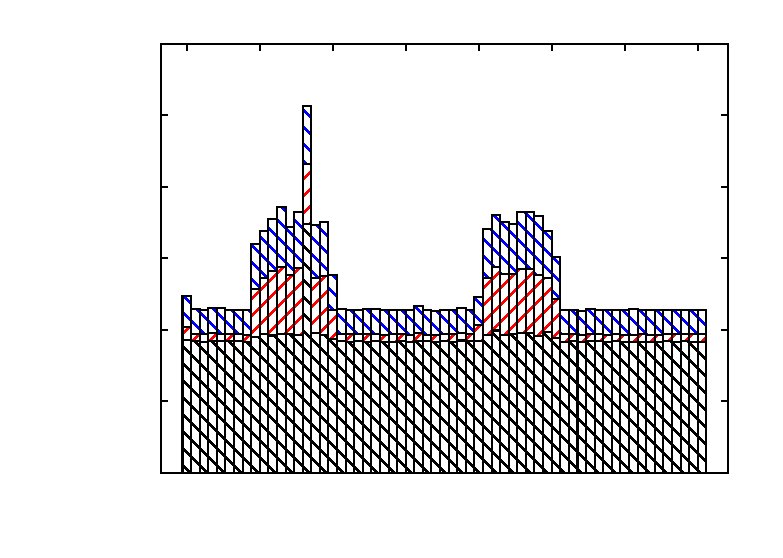
\includegraphics{fig/rtaiEsc}}%
    \gplfronttext
  \end{picture}%
\endgroup
}}}\\
  \vspace{20pt}
  \subfloat[Lat�ncias do Xenomai]{%
    \label{fig:xenoEsc}%
    {\scalebox{0.9}{% GNUPLOT: LaTeX picture with Postscript
\begingroup
  \makeatletter
  \providecommand\color[2][]{%
    \GenericError{(gnuplot) \space\space\space\@spaces}{%
      Package color not loaded in conjunction with
      terminal option `colourtext'%
    }{See the gnuplot documentation for explanation.%
    }{Either use 'blacktext' in gnuplot or load the package
      color.sty in LaTeX.}%
    \renewcommand\color[2][]{}%
  }%
  \providecommand\includegraphics[2][]{%
    \GenericError{(gnuplot) \space\space\space\@spaces}{%
      Package graphicx or graphics not loaded%
    }{See the gnuplot documentation for explanation.%
    }{The gnuplot epslatex terminal needs graphicx.sty or graphics.sty.}%
    \renewcommand\includegraphics[2][]{}%
  }%
  \providecommand\rotatebox[2]{#2}%
  \@ifundefined{ifGPcolor}{%
    \newif\ifGPcolor
    \GPcolorfalse
  }{}%
  \@ifundefined{ifGPblacktext}{%
    \newif\ifGPblacktext
    \GPblacktextfalse
  }{}%
  % define a \g@addto@macro without @ in the name:
  \let\gplgaddtomacro\g@addto@macro
  % define empty templates for all commands taking text:
  \gdef\gplbacktext{}%
  \gdef\gplfronttext{}%
  \makeatother
  \ifGPblacktext
    % no textcolor at all
    \def\colorrgb#1{}%
    \def\colorgray#1{}%
  \else
    % gray or color?
    \ifGPcolor
      \def\colorrgb#1{\color[rgb]{#1}}%
      \def\colorgray#1{\color[gray]{#1}}%
      \expandafter\def\csname LTw\endcsname{\color{white}}%
      \expandafter\def\csname LTb\endcsname{\color{black}}%
      \expandafter\def\csname LTa\endcsname{\color{black}}%
      \expandafter\def\csname LT0\endcsname{\color[rgb]{1,0,0}}%
      \expandafter\def\csname LT1\endcsname{\color[rgb]{0,1,0}}%
      \expandafter\def\csname LT2\endcsname{\color[rgb]{0,0,1}}%
      \expandafter\def\csname LT3\endcsname{\color[rgb]{1,0,1}}%
      \expandafter\def\csname LT4\endcsname{\color[rgb]{0,1,1}}%
      \expandafter\def\csname LT5\endcsname{\color[rgb]{1,1,0}}%
      \expandafter\def\csname LT6\endcsname{\color[rgb]{0,0,0}}%
      \expandafter\def\csname LT7\endcsname{\color[rgb]{1,0.3,0}}%
      \expandafter\def\csname LT8\endcsname{\color[rgb]{0.5,0.5,0.5}}%
    \else
      % gray
      \def\colorrgb#1{\color{black}}%
      \def\colorgray#1{\color[gray]{#1}}%
      \expandafter\def\csname LTw\endcsname{\color{white}}%
      \expandafter\def\csname LTb\endcsname{\color{black}}%
      \expandafter\def\csname LTa\endcsname{\color{black}}%
      \expandafter\def\csname LT0\endcsname{\color{black}}%
      \expandafter\def\csname LT1\endcsname{\color{black}}%
      \expandafter\def\csname LT2\endcsname{\color{black}}%
      \expandafter\def\csname LT3\endcsname{\color{black}}%
      \expandafter\def\csname LT4\endcsname{\color{black}}%
      \expandafter\def\csname LT5\endcsname{\color{black}}%
      \expandafter\def\csname LT6\endcsname{\color{black}}%
      \expandafter\def\csname LT7\endcsname{\color{black}}%
      \expandafter\def\csname LT8\endcsname{\color{black}}%
    \fi
  \fi
  \setlength{\unitlength}{0.0500bp}%
  \begin{picture}(7200.00,5040.00)%
    \gplgaddtomacro\gplbacktext{%
      \csname LTb\endcsname%
      \put(1254,660){\makebox(0,0)[r]{\strut{}$0.0$}}%
      \put(1254,1346){\makebox(0,0)[r]{\strut{}$5.0$}}%
      \put(1254,2032){\makebox(0,0)[r]{\strut{}$10.0$}}%
      \put(1254,2718){\makebox(0,0)[r]{\strut{}$15.0$}}%
      \put(1254,3404){\makebox(0,0)[r]{\strut{}$20.0$}}%
      \put(1254,4090){\makebox(0,0)[r]{\strut{}$25.0$}}%
      \put(1254,4776){\makebox(0,0)[r]{\strut{}$30.0$}}%
      \put(1633,440){\makebox(0,0){\strut{}0}}%
      \put(2334,440){\makebox(0,0){\strut{}10}}%
      \put(3034,440){\makebox(0,0){\strut{}20}}%
      \put(3735,440){\makebox(0,0){\strut{}30}}%
      \put(4436,440){\makebox(0,0){\strut{}40}}%
      \put(5136,440){\makebox(0,0){\strut{}50}}%
      \put(5837,440){\makebox(0,0){\strut{}60}}%
      \put(6538,440){\makebox(0,0){\strut{}70}}%
      \put(220,2718){\rotatebox{90}{\makebox(0,0){\strut{}Lat\^encia em $\mu s$}}}%
      \put(4106,110){\makebox(0,0){\strut{}Tempo de execu\c{c}\~ao em $s$}}%
    }%
    \gplgaddtomacro\gplfronttext{%
    }%
    \gplbacktext
    \put(0,0){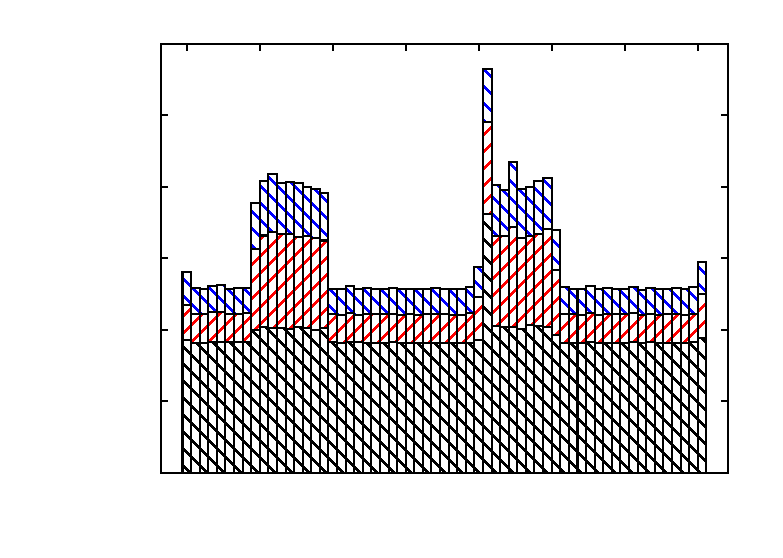
\includegraphics{fig/xenoEsc}}%
    \gplfronttext
  \end{picture}%
\endgroup
}}}\\
  \caption[Lat�ncia de interrup��o, de escalonamento e de execu��o do RTAI e do
  Xenomai]{Lat�ncia de interrup��o de escalonamento e de execu��o do Kernel Linux
    vers�o 2.6.19.7, com o \ing{patch} $RTAI$ e com o \ing{patch} Xenomai. As
    figuras \subref{fig:rtaiEsc} e \subref{fig:xenoEsc} apresentam as tr�s
    lat�ncias, na forma de histogramas sobreposto um em cima do outro.  A base
    coresponde a lat�ncia de interrup��o, a caixa do meio, a lat�ncia de
    escalonamento e a caixa de cima a lat�ncia de execu��o. Em ambos experimentos, a
    freq��ncia de interrup��o � $20 Hz$ e o canal RT-FIFO � consultado e as m�dias
    correspondentes calculadas a cada 20 eventos. Os dois estresses (60 aberturas e
    fechamento de sess�o \cod{ssh}) s�o aplicados nos instantes 10s e 40s.}
  \label{fig:latEscal}%
\end{figure}

Para observar o efeito do estresse sobre a lat�ncia de escalonamento e o tempo de
execu��o da tarefa $T$, a figura \ref{fig:stress} apresenta o detalhe das medidas
destes dois valores correspondendo aos experimentos das figuras
\ref{fig:rtai}\subref{fig:rtai2} e \ref{fig:xeno}\subref{fig:xeno1}.  Constata-se
que as duas plataformas comportam-se de forma bastante similares, com um aumento de
aproximadamente $4 \mu s$ na lat�ncia de interrup��o e de $2$ a $3 \mu s$ no tempo
de execu��o. O primeiro aumento corresponde provavelmente ao tratamento de uma (ou
duas nos piores casos) interrup��o da placa de rede, devida ao estresse. A segunda,
por ser mais espalhadas e ter valores menores, corresponde provavelmente a
atualiza��o da mem�ria tamp�o.

\begin{figure}%
  \centering
  \subfloat[][RTAI]{%
    \label{fig:rtaiStress}%
    {\scalebox{1}{% GNUPLOT: LaTeX picture with Postscript
\begingroup
  \makeatletter
  \providecommand\color[2][]{%
    \GenericError{(gnuplot) \space\space\space\@spaces}{%
      Package color not loaded in conjunction with
      terminal option `colourtext'%
    }{See the gnuplot documentation for explanation.%
    }{Either use 'blacktext' in gnuplot or load the package
      color.sty in LaTeX.}%
    \renewcommand\color[2][]{}%
  }%
  \providecommand\includegraphics[2][]{%
    \GenericError{(gnuplot) \space\space\space\@spaces}{%
      Package graphicx or graphics not loaded%
    }{See the gnuplot documentation for explanation.%
    }{The gnuplot epslatex terminal needs graphicx.sty or graphics.sty.}%
    \renewcommand\includegraphics[2][]{}%
  }%
  \providecommand\rotatebox[2]{#2}%
  \@ifundefined{ifGPcolor}{%
    \newif\ifGPcolor
    \GPcolorfalse
  }{}%
  \@ifundefined{ifGPblacktext}{%
    \newif\ifGPblacktext
    \GPblacktextfalse
  }{}%
  % define a \g@addto@macro without @ in the name:
  \let\gplgaddtomacro\g@addto@macro
  % define empty templates for all commands taking text:
  \gdef\gplbacktext{}%
  \gdef\gplfronttext{}%
  \makeatother
  \ifGPblacktext
    % no textcolor at all
    \def\colorrgb#1{}%
    \def\colorgray#1{}%
  \else
    % gray or color?
    \ifGPcolor
      \def\colorrgb#1{\color[rgb]{#1}}%
      \def\colorgray#1{\color[gray]{#1}}%
      \expandafter\def\csname LTw\endcsname{\color{white}}%
      \expandafter\def\csname LTb\endcsname{\color{black}}%
      \expandafter\def\csname LTa\endcsname{\color{black}}%
      \expandafter\def\csname LT0\endcsname{\color[rgb]{1,0,0}}%
      \expandafter\def\csname LT1\endcsname{\color[rgb]{0,1,0}}%
      \expandafter\def\csname LT2\endcsname{\color[rgb]{0,0,1}}%
      \expandafter\def\csname LT3\endcsname{\color[rgb]{1,0,1}}%
      \expandafter\def\csname LT4\endcsname{\color[rgb]{0,1,1}}%
      \expandafter\def\csname LT5\endcsname{\color[rgb]{1,1,0}}%
      \expandafter\def\csname LT6\endcsname{\color[rgb]{0,0,0}}%
      \expandafter\def\csname LT7\endcsname{\color[rgb]{1,0.3,0}}%
      \expandafter\def\csname LT8\endcsname{\color[rgb]{0.5,0.5,0.5}}%
    \else
      % gray
      \def\colorrgb#1{\color{black}}%
      \def\colorgray#1{\color[gray]{#1}}%
      \expandafter\def\csname LTw\endcsname{\color{white}}%
      \expandafter\def\csname LTb\endcsname{\color{black}}%
      \expandafter\def\csname LTa\endcsname{\color{black}}%
      \expandafter\def\csname LT0\endcsname{\color{black}}%
      \expandafter\def\csname LT1\endcsname{\color{black}}%
      \expandafter\def\csname LT2\endcsname{\color{black}}%
      \expandafter\def\csname LT3\endcsname{\color{black}}%
      \expandafter\def\csname LT4\endcsname{\color{black}}%
      \expandafter\def\csname LT5\endcsname{\color{black}}%
      \expandafter\def\csname LT6\endcsname{\color{black}}%
      \expandafter\def\csname LT7\endcsname{\color{black}}%
      \expandafter\def\csname LT8\endcsname{\color{black}}%
    \fi
  \fi
  \setlength{\unitlength}{0.0500bp}%
  \begin{picture}(7200.00,5040.00)%
    \gplgaddtomacro\gplbacktext{%
      \csname LTb\endcsname%
      \put(1254,660){\makebox(0,0)[r]{\strut{}$0.0$}}%
      \put(1254,1346){\makebox(0,0)[r]{\strut{}$2.0$}}%
      \put(1254,2032){\makebox(0,0)[r]{\strut{}$4.0$}}%
      \put(1254,2718){\makebox(0,0)[r]{\strut{}$6.0$}}%
      \put(1254,3404){\makebox(0,0)[r]{\strut{}$8.0$}}%
      \put(1254,4090){\makebox(0,0)[r]{\strut{}$10.0$}}%
      \put(1254,4776){\makebox(0,0)[r]{\strut{}$12.0$}}%
      \put(1386,440){\makebox(0,0){\strut{}$ 5$}}%
      \put(2746,440){\makebox(0,0){\strut{}$ 10$}}%
      \put(4106,440){\makebox(0,0){\strut{}$ 15$}}%
      \put(5466,440){\makebox(0,0){\strut{}$ 20$}}%
      \put(6826,440){\makebox(0,0){\strut{}$ 25$}}%
      \put(220,2718){\rotatebox{90}{\makebox(0,0){\strut{}Lat\^encia em $\mu s$}}}%
      \put(4106,110){\makebox(0,0){\strut{}Tempo de execu\c{c}\~ao em $s$}}%
    }%
    \gplgaddtomacro\gplfronttext{%
      \csname LTb\endcsname%
      \put(6243,4323){\makebox(0,0)[r]{\strut{}Escalonamento}}%
      \csname LTb\endcsname%
      \put(6243,4103){\makebox(0,0)[r]{\strut{}Execu\c{c}\~ao}}%
    }%
    \gplbacktext
    \put(0,0){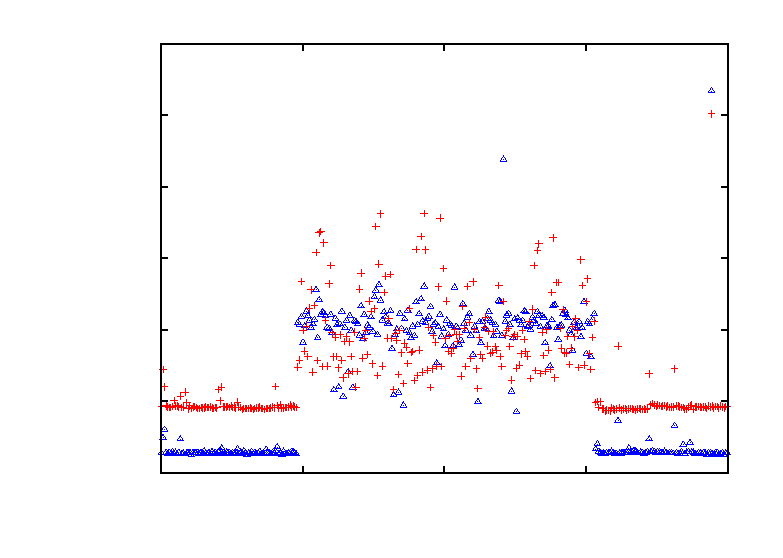
\includegraphics{fig/rtaiStress}}%
    \gplfronttext
  \end{picture}%
\endgroup
}}}%
   \hspace{14pt}%
  \subfloat[][Xenomai]{%
    \label{fig:xenoStress}%
    {\scalebox{1}{% GNUPLOT: LaTeX picture with Postscript
\begingroup
  \makeatletter
  \providecommand\color[2][]{%
    \GenericError{(gnuplot) \space\space\space\@spaces}{%
      Package color not loaded in conjunction with
      terminal option `colourtext'%
    }{See the gnuplot documentation for explanation.%
    }{Either use 'blacktext' in gnuplot or load the package
      color.sty in LaTeX.}%
    \renewcommand\color[2][]{}%
  }%
  \providecommand\includegraphics[2][]{%
    \GenericError{(gnuplot) \space\space\space\@spaces}{%
      Package graphicx or graphics not loaded%
    }{See the gnuplot documentation for explanation.%
    }{The gnuplot epslatex terminal needs graphicx.sty or graphics.sty.}%
    \renewcommand\includegraphics[2][]{}%
  }%
  \providecommand\rotatebox[2]{#2}%
  \@ifundefined{ifGPcolor}{%
    \newif\ifGPcolor
    \GPcolorfalse
  }{}%
  \@ifundefined{ifGPblacktext}{%
    \newif\ifGPblacktext
    \GPblacktextfalse
  }{}%
  % define a \g@addto@macro without @ in the name:
  \let\gplgaddtomacro\g@addto@macro
  % define empty templates for all commands taking text:
  \gdef\gplbacktext{}%
  \gdef\gplfronttext{}%
  \makeatother
  \ifGPblacktext
    % no textcolor at all
    \def\colorrgb#1{}%
    \def\colorgray#1{}%
  \else
    % gray or color?
    \ifGPcolor
      \def\colorrgb#1{\color[rgb]{#1}}%
      \def\colorgray#1{\color[gray]{#1}}%
      \expandafter\def\csname LTw\endcsname{\color{white}}%
      \expandafter\def\csname LTb\endcsname{\color{black}}%
      \expandafter\def\csname LTa\endcsname{\color{black}}%
      \expandafter\def\csname LT0\endcsname{\color[rgb]{1,0,0}}%
      \expandafter\def\csname LT1\endcsname{\color[rgb]{0,1,0}}%
      \expandafter\def\csname LT2\endcsname{\color[rgb]{0,0,1}}%
      \expandafter\def\csname LT3\endcsname{\color[rgb]{1,0,1}}%
      \expandafter\def\csname LT4\endcsname{\color[rgb]{0,1,1}}%
      \expandafter\def\csname LT5\endcsname{\color[rgb]{1,1,0}}%
      \expandafter\def\csname LT6\endcsname{\color[rgb]{0,0,0}}%
      \expandafter\def\csname LT7\endcsname{\color[rgb]{1,0.3,0}}%
      \expandafter\def\csname LT8\endcsname{\color[rgb]{0.5,0.5,0.5}}%
    \else
      % gray
      \def\colorrgb#1{\color{black}}%
      \def\colorgray#1{\color[gray]{#1}}%
      \expandafter\def\csname LTw\endcsname{\color{white}}%
      \expandafter\def\csname LTb\endcsname{\color{black}}%
      \expandafter\def\csname LTa\endcsname{\color{black}}%
      \expandafter\def\csname LT0\endcsname{\color{black}}%
      \expandafter\def\csname LT1\endcsname{\color{black}}%
      \expandafter\def\csname LT2\endcsname{\color{black}}%
      \expandafter\def\csname LT3\endcsname{\color{black}}%
      \expandafter\def\csname LT4\endcsname{\color{black}}%
      \expandafter\def\csname LT5\endcsname{\color{black}}%
      \expandafter\def\csname LT6\endcsname{\color{black}}%
      \expandafter\def\csname LT7\endcsname{\color{black}}%
      \expandafter\def\csname LT8\endcsname{\color{black}}%
    \fi
  \fi
  \setlength{\unitlength}{0.0500bp}%
  \begin{picture}(7200.00,5040.00)%
    \gplgaddtomacro\gplbacktext{%
      \csname LTb\endcsname%
      \put(1254,660){\makebox(0,0)[r]{\strut{}$1.0$}}%
      \put(1254,1034){\makebox(0,0)[r]{\strut{}$2.0$}}%
      \put(1254,1408){\makebox(0,0)[r]{\strut{}$3.0$}}%
      \put(1254,1783){\makebox(0,0)[r]{\strut{}$4.0$}}%
      \put(1254,2157){\makebox(0,0)[r]{\strut{}$5.0$}}%
      \put(1254,2531){\makebox(0,0)[r]{\strut{}$6.0$}}%
      \put(1254,2905){\makebox(0,0)[r]{\strut{}$7.0$}}%
      \put(1254,3279){\makebox(0,0)[r]{\strut{}$8.0$}}%
      \put(1254,3653){\makebox(0,0)[r]{\strut{}$9.0$}}%
      \put(1254,4028){\makebox(0,0)[r]{\strut{}$10.0$}}%
      \put(1254,4402){\makebox(0,0)[r]{\strut{}$11.0$}}%
      \put(1254,4776){\makebox(0,0)[r]{\strut{}$12.0$}}%
      \put(1386,440){\makebox(0,0){\strut{}$ 5$}}%
      \put(2746,440){\makebox(0,0){\strut{}$ 10$}}%
      \put(4106,440){\makebox(0,0){\strut{}$ 15$}}%
      \put(5466,440){\makebox(0,0){\strut{}$ 20$}}%
      \put(6826,440){\makebox(0,0){\strut{}$ 25$}}%
      \put(220,2718){\rotatebox{90}{\makebox(0,0){\strut{}Lat\^encia em $\mu s$}}}%
      \put(4106,110){\makebox(0,0){\strut{}Tempo de execu\c{c}\~ao em $s$}}%
    }%
    \gplgaddtomacro\gplfronttext{%
      \csname LTb\endcsname%
      \put(6107,4367){\makebox(0,0)[r]{\strut{}Escalonamento}}%
      \csname LTb\endcsname%
      \put(6107,4147){\makebox(0,0)[r]{\strut{}Execu\c{c}\~ao}}%
    }%
    \gplbacktext
    \put(0,0){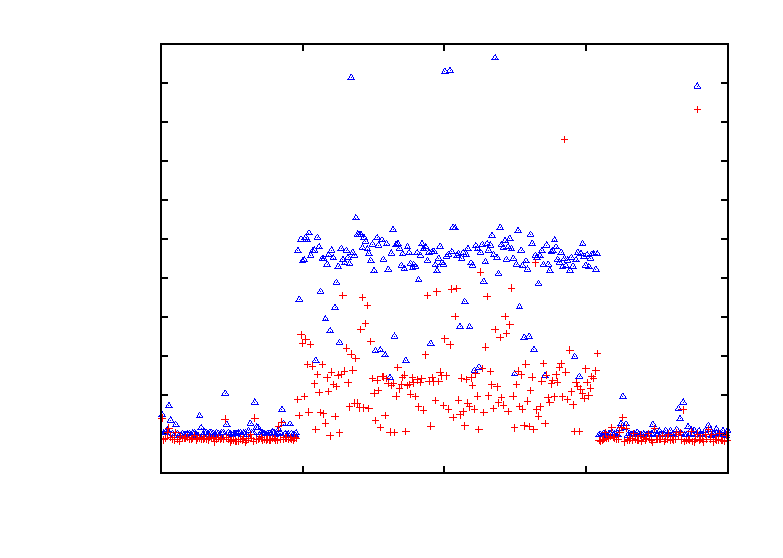
\includegraphics{fig/xenoStress}}%
    \gplfronttext
  \end{picture}%
\endgroup
}}}%
%   \hspace{14pt}%
%   \subfloat[][M�dia sobre 50 eventos, freq��ncia de $1000 Hz$.]{%
%     \label{fig:xenoF1}%
%     {\scalebox{0.6}{\input{fig/xenoF1}}}}%
  \caption[Lat�ncia de escalonamento e de execu��o de RTAI e Xenomai]{Lat�ncia de
    escalonamento e tempo de execu��es do Kernel Linux 2.6.19.7, com RTAI e com
    Xenomai. As figuras \subref{fig:rtaiStress} e \subref{fig:xenoStress}
    representam detalhes das figuras \ref{fig:rtai}\subref{fig:rtai2} e
    \ref{fig:xeno}\subref{fig:xeno1}.}
  \label{fig:stress}%
\end{figure}








A interpreta��o proposta aqui para os resultados relativos ao estresse UDP � a
seguinte.  Quando a placa de rede recebe um pacote Ethernet, ela gera uma
interrup��o para informar o processador. Este eventualmente executa o tratador
associado a esta interrup��o. Mas, se um novo pacote cheguar antes do fim da sua
execu��o, o tratador poderia ser preemptado por uma outra execu��o dele mesmo.  Para
prevenir esta eventualidade, foi visto na se��o \label{sec:interrupt} que o \kernell
padr�o desabilita as interrup��es durante a execu��o de um tratador de
interrup��o. Al�m disso, durante a execu��o do tratador, quando o \kernell percebe
que v�rios pacotes est�o esperando na mem�ria tamp�o da placa, uma otimiza��o da
camada de rede permite que estes v�rios pacotes sejam recebidos, sem esperar novas
interrup��es. Estas opera��es acumuladas podem explicar que as interrup��es sejam
desabilitadas para tempos mais longo que o tempo de recep��o de um pacote s�.

\begin{figure}[!hbt]
  %\hfill
  %\vspace{0.2in}
  \begin{minipage}[!t]{\textwidth}
    \begin{center}  
      \centerline{\resizebox{0.8\linewidth}{!}{% GNUPLOT: LaTeX picture with Postscript
\begingroup
  \makeatletter
  \providecommand\color[2][]{%
    \GenericError{(gnuplot) \space\space\space\@spaces}{%
      Package color not loaded in conjunction with
      terminal option `colourtext'%
    }{See the gnuplot documentation for explanation.%
    }{Either use 'blacktext' in gnuplot or load the package
      color.sty in LaTeX.}%
    \renewcommand\color[2][]{}%
  }%
  \providecommand\includegraphics[2][]{%
    \GenericError{(gnuplot) \space\space\space\@spaces}{%
      Package graphicx or graphics not loaded%
    }{See the gnuplot documentation for explanation.%
    }{The gnuplot epslatex terminal needs graphicx.sty or graphics.sty.}%
    \renewcommand\includegraphics[2][]{}%
  }%
  \providecommand\rotatebox[2]{#2}%
  \@ifundefined{ifGPcolor}{%
    \newif\ifGPcolor
    \GPcolorfalse
  }{}%
  \@ifundefined{ifGPblacktext}{%
    \newif\ifGPblacktext
    \GPblacktextfalse
  }{}%
  % define a \g@addto@macro without @ in the name:
  \let\gplgaddtomacro\g@addto@macro
  % define empty templates for all commands taking text:
  \gdef\gplbacktext{}%
  \gdef\gplfronttext{}%
  \makeatother
  \ifGPblacktext
    % no textcolor at all
    \def\colorrgb#1{}%
    \def\colorgray#1{}%
  \else
    % gray or color?
    \ifGPcolor
      \def\colorrgb#1{\color[rgb]{#1}}%
      \def\colorgray#1{\color[gray]{#1}}%
      \expandafter\def\csname LTw\endcsname{\color{white}}%
      \expandafter\def\csname LTb\endcsname{\color{black}}%
      \expandafter\def\csname LTa\endcsname{\color{black}}%
      \expandafter\def\csname LT0\endcsname{\color[rgb]{1,0,0}}%
      \expandafter\def\csname LT1\endcsname{\color[rgb]{0,1,0}}%
      \expandafter\def\csname LT2\endcsname{\color[rgb]{0,0,1}}%
      \expandafter\def\csname LT3\endcsname{\color[rgb]{1,0,1}}%
      \expandafter\def\csname LT4\endcsname{\color[rgb]{0,1,1}}%
      \expandafter\def\csname LT5\endcsname{\color[rgb]{1,1,0}}%
      \expandafter\def\csname LT6\endcsname{\color[rgb]{0,0,0}}%
      \expandafter\def\csname LT7\endcsname{\color[rgb]{1,0.3,0}}%
      \expandafter\def\csname LT8\endcsname{\color[rgb]{0.5,0.5,0.5}}%
    \else
      % gray
      \def\colorrgb#1{\color{black}}%
      \def\colorgray#1{\color[gray]{#1}}%
      \expandafter\def\csname LTw\endcsname{\color{white}}%
      \expandafter\def\csname LTb\endcsname{\color{black}}%
      \expandafter\def\csname LTa\endcsname{\color{black}}%
      \expandafter\def\csname LT0\endcsname{\color{black}}%
      \expandafter\def\csname LT1\endcsname{\color{black}}%
      \expandafter\def\csname LT2\endcsname{\color{black}}%
      \expandafter\def\csname LT3\endcsname{\color{black}}%
      \expandafter\def\csname LT4\endcsname{\color{black}}%
      \expandafter\def\csname LT5\endcsname{\color{black}}%
      \expandafter\def\csname LT6\endcsname{\color{black}}%
      \expandafter\def\csname LT7\endcsname{\color{black}}%
      \expandafter\def\csname LT8\endcsname{\color{black}}%
    \fi
  \fi
  \setlength{\unitlength}{0.0500bp}%
  \begin{picture}(7200.00,5040.00)%
    \gplgaddtomacro\gplbacktext{%
      \csname LTb\endcsname%
      \put(1386,660){\makebox(0,0)[r]{\strut{}$0.0$}}%
      \put(1386,1280){\makebox(0,0)[r]{\strut{}$20.0$}}%
      \put(1386,1900){\makebox(0,0)[r]{\strut{}$40.0$}}%
      \put(1386,2520){\makebox(0,0)[r]{\strut{}$60.0$}}%
      \put(1386,3140){\makebox(0,0)[r]{\strut{}$80.0$}}%
      \put(1386,3760){\makebox(0,0)[r]{\strut{}$100.0$}}%
      \put(1386,4380){\makebox(0,0)[r]{\strut{}$120.0$}}%
      \put(1518,440){\makebox(0,0){\strut{}$ 0$}}%
      \put(2276,440){\makebox(0,0){\strut{}$ 10$}}%
      \put(3035,440){\makebox(0,0){\strut{}$ 20$}}%
      \put(3793,440){\makebox(0,0){\strut{}$ 30$}}%
      \put(4551,440){\makebox(0,0){\strut{}$ 40$}}%
      \put(5309,440){\makebox(0,0){\strut{}$ 50$}}%
      \put(6068,440){\makebox(0,0){\strut{}$ 60$}}%
      \put(6826,440){\makebox(0,0){\strut{}$ 70$}}%
      \put(220,2520){\rotatebox{90}{\makebox(0,0){\strut{}Lat\^encia em $\mu s$}}}%
      \put(4172,110){\makebox(0,0){\strut{}Tempo de execu\c{c}\~ao em $s$}}%
      \put(4172,4710){\makebox(0,0){\strut{}Kernel Linux - Lat\^encia de interrup\c{c}\~ao}}%
    }%
    \gplgaddtomacro\gplfronttext{%
    }%
    \gplbacktext
    \put(0,0){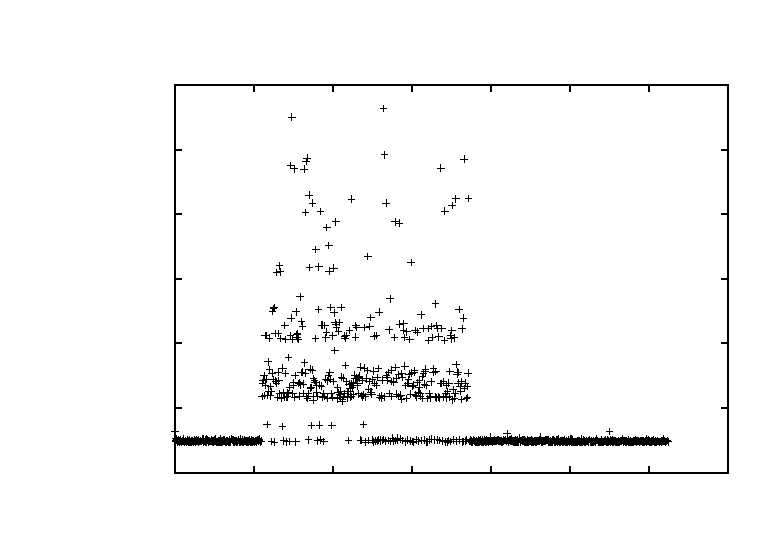
\includegraphics{fig/irqKern}}%
    \gplfronttext
  \end{picture}%
\endgroup
}}
      \caption{Lat�ncia de interrup��o do \kernell Linux}
      \label{fig:irqKern}
    \end{center}
  \end{minipage}
  %\hfill
  \\
  \vspace{.4in}
  \begin{minipage}[!t]{\textwidth}
    \begin{center}  
      \centerline{\resizebox{0.8\linewidth}{!}{% GNUPLOT: LaTeX picture with Postscript
\begingroup
  \makeatletter
  \providecommand\color[2][]{%
    \GenericError{(gnuplot) \space\space\space\@spaces}{%
      Package color not loaded in conjunction with
      terminal option `colourtext'%
    }{See the gnuplot documentation for explanation.%
    }{Either use 'blacktext' in gnuplot or load the package
      color.sty in LaTeX.}%
    \renewcommand\color[2][]{}%
  }%
  \providecommand\includegraphics[2][]{%
    \GenericError{(gnuplot) \space\space\space\@spaces}{%
      Package graphicx or graphics not loaded%
    }{See the gnuplot documentation for explanation.%
    }{The gnuplot epslatex terminal needs graphicx.sty or graphics.sty.}%
    \renewcommand\includegraphics[2][]{}%
  }%
  \providecommand\rotatebox[2]{#2}%
  \@ifundefined{ifGPcolor}{%
    \newif\ifGPcolor
    \GPcolorfalse
  }{}%
  \@ifundefined{ifGPblacktext}{%
    \newif\ifGPblacktext
    \GPblacktextfalse
  }{}%
  % define a \g@addto@macro without @ in the name:
  \let\gplgaddtomacro\g@addto@macro
  % define empty templates for all commands taking text:
  \gdef\gplbacktext{}%
  \gdef\gplfronttext{}%
  \makeatother
  \ifGPblacktext
    % no textcolor at all
    \def\colorrgb#1{}%
    \def\colorgray#1{}%
  \else
    % gray or color?
    \ifGPcolor
      \def\colorrgb#1{\color[rgb]{#1}}%
      \def\colorgray#1{\color[gray]{#1}}%
      \expandafter\def\csname LTw\endcsname{\color{white}}%
      \expandafter\def\csname LTb\endcsname{\color{black}}%
      \expandafter\def\csname LTa\endcsname{\color{black}}%
      \expandafter\def\csname LT0\endcsname{\color[rgb]{1,0,0}}%
      \expandafter\def\csname LT1\endcsname{\color[rgb]{0,1,0}}%
      \expandafter\def\csname LT2\endcsname{\color[rgb]{0,0,1}}%
      \expandafter\def\csname LT3\endcsname{\color[rgb]{1,0,1}}%
      \expandafter\def\csname LT4\endcsname{\color[rgb]{0,1,1}}%
      \expandafter\def\csname LT5\endcsname{\color[rgb]{1,1,0}}%
      \expandafter\def\csname LT6\endcsname{\color[rgb]{0,0,0}}%
      \expandafter\def\csname LT7\endcsname{\color[rgb]{1,0.3,0}}%
      \expandafter\def\csname LT8\endcsname{\color[rgb]{0.5,0.5,0.5}}%
    \else
      % gray
      \def\colorrgb#1{\color{black}}%
      \def\colorgray#1{\color[gray]{#1}}%
      \expandafter\def\csname LTw\endcsname{\color{white}}%
      \expandafter\def\csname LTb\endcsname{\color{black}}%
      \expandafter\def\csname LTa\endcsname{\color{black}}%
      \expandafter\def\csname LT0\endcsname{\color{black}}%
      \expandafter\def\csname LT1\endcsname{\color{black}}%
      \expandafter\def\csname LT2\endcsname{\color{black}}%
      \expandafter\def\csname LT3\endcsname{\color{black}}%
      \expandafter\def\csname LT4\endcsname{\color{black}}%
      \expandafter\def\csname LT5\endcsname{\color{black}}%
      \expandafter\def\csname LT6\endcsname{\color{black}}%
      \expandafter\def\csname LT7\endcsname{\color{black}}%
      \expandafter\def\csname LT8\endcsname{\color{black}}%
    \fi
  \fi
  \setlength{\unitlength}{0.0500bp}%
  \begin{picture}(7200.00,5040.00)%
    \gplgaddtomacro\gplbacktext{%
      \csname LTb\endcsname%
      \put(1254,660){\makebox(0,0)[r]{\strut{}$0.0$}}%
      \put(1254,1125){\makebox(0,0)[r]{\strut{}$10.0$}}%
      \put(1254,1590){\makebox(0,0)[r]{\strut{}$20.0$}}%
      \put(1254,2055){\makebox(0,0)[r]{\strut{}$30.0$}}%
      \put(1254,2520){\makebox(0,0)[r]{\strut{}$40.0$}}%
      \put(1254,2985){\makebox(0,0)[r]{\strut{}$50.0$}}%
      \put(1254,3450){\makebox(0,0)[r]{\strut{}$60.0$}}%
      \put(1254,3915){\makebox(0,0)[r]{\strut{}$70.0$}}%
      \put(1254,4380){\makebox(0,0)[r]{\strut{}$80.0$}}%
      \put(1386,440){\makebox(0,0){\strut{}$ 0$}}%
      \put(2293,440){\makebox(0,0){\strut{}$ 10$}}%
      \put(3199,440){\makebox(0,0){\strut{}$ 20$}}%
      \put(4106,440){\makebox(0,0){\strut{}$ 30$}}%
      \put(5013,440){\makebox(0,0){\strut{}$ 40$}}%
      \put(5919,440){\makebox(0,0){\strut{}$ 50$}}%
      \put(6826,440){\makebox(0,0){\strut{}$ 60$}}%
      \put(220,2520){\rotatebox{90}{\makebox(0,0){\strut{}Lat\^encia em $\mu s$}}}%
      \put(4106,110){\makebox(0,0){\strut{}Tempo de execu\c{c}\~ao em $s$}}%
      \put(4106,4710){\makebox(0,0){\strut{}Kernel Linux - Lat\^encia de interrup\c{c}\~ao (m�dia)}}%
      \put(5013,3450){\makebox(0,0)[l]{\strut{}Desvio padr\~ao}}%
      \put(5013,3230){\makebox(0,0)[l]{\strut{}m\'{a}ximo 124.6}}%
    }%
    \gplgaddtomacro\gplfronttext{%
    }%
    \gplbacktext
    \put(0,0){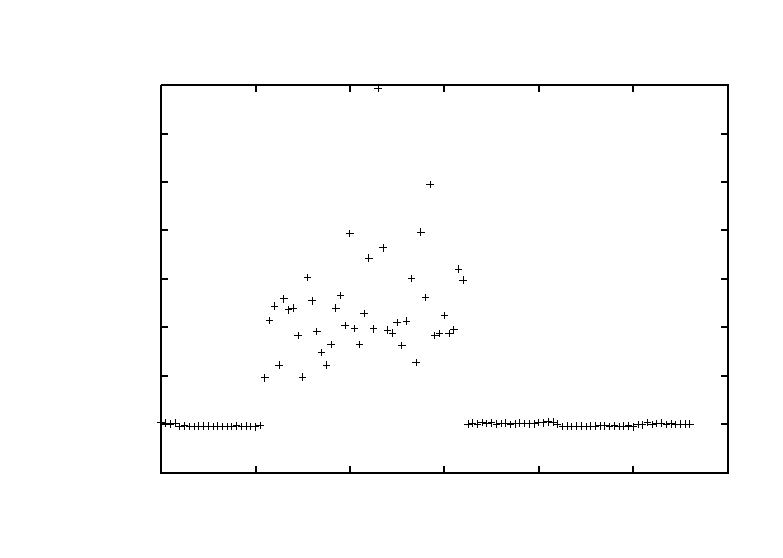
\includegraphics{fig/irqKernMean}}%
    \gplfronttext
  \end{picture}%
\endgroup
}}
      \caption{Lat�ncia de interrup��o do \kernell Linux (m�dia sobre 10 valores)}
      \label{fig:irqKernMean}
    \end{center}
  \end{minipage}
  %\hfill
\end{figure}

\begin{figure}[!hbt]
  %\hfill
  %\vspace{0.2in}
  \begin{minipage}[!t]{\textwidth}
    \begin{center}  
      \centerline{\resizebox{0.8\linewidth}{!}{% GNUPLOT: LaTeX picture with Postscript
\begingroup
  \makeatletter
  \providecommand\color[2][]{%
    \GenericError{(gnuplot) \space\space\space\@spaces}{%
      Package color not loaded in conjunction with
      terminal option `colourtext'%
    }{See the gnuplot documentation for explanation.%
    }{Either use 'blacktext' in gnuplot or load the package
      color.sty in LaTeX.}%
    \renewcommand\color[2][]{}%
  }%
  \providecommand\includegraphics[2][]{%
    \GenericError{(gnuplot) \space\space\space\@spaces}{%
      Package graphicx or graphics not loaded%
    }{See the gnuplot documentation for explanation.%
    }{The gnuplot epslatex terminal needs graphicx.sty or graphics.sty.}%
    \renewcommand\includegraphics[2][]{}%
  }%
  \providecommand\rotatebox[2]{#2}%
  \@ifundefined{ifGPcolor}{%
    \newif\ifGPcolor
    \GPcolorfalse
  }{}%
  \@ifundefined{ifGPblacktext}{%
    \newif\ifGPblacktext
    \GPblacktextfalse
  }{}%
  % define a \g@addto@macro without @ in the name:
  \let\gplgaddtomacro\g@addto@macro
  % define empty templates for all commands taking text:
  \gdef\gplbacktext{}%
  \gdef\gplfronttext{}%
  \makeatother
  \ifGPblacktext
    % no textcolor at all
    \def\colorrgb#1{}%
    \def\colorgray#1{}%
  \else
    % gray or color?
    \ifGPcolor
      \def\colorrgb#1{\color[rgb]{#1}}%
      \def\colorgray#1{\color[gray]{#1}}%
      \expandafter\def\csname LTw\endcsname{\color{white}}%
      \expandafter\def\csname LTb\endcsname{\color{black}}%
      \expandafter\def\csname LTa\endcsname{\color{black}}%
      \expandafter\def\csname LT0\endcsname{\color[rgb]{1,0,0}}%
      \expandafter\def\csname LT1\endcsname{\color[rgb]{0,1,0}}%
      \expandafter\def\csname LT2\endcsname{\color[rgb]{0,0,1}}%
      \expandafter\def\csname LT3\endcsname{\color[rgb]{1,0,1}}%
      \expandafter\def\csname LT4\endcsname{\color[rgb]{0,1,1}}%
      \expandafter\def\csname LT5\endcsname{\color[rgb]{1,1,0}}%
      \expandafter\def\csname LT6\endcsname{\color[rgb]{0,0,0}}%
      \expandafter\def\csname LT7\endcsname{\color[rgb]{1,0.3,0}}%
      \expandafter\def\csname LT8\endcsname{\color[rgb]{0.5,0.5,0.5}}%
    \else
      % gray
      \def\colorrgb#1{\color{black}}%
      \def\colorgray#1{\color[gray]{#1}}%
      \expandafter\def\csname LTw\endcsname{\color{white}}%
      \expandafter\def\csname LTb\endcsname{\color{black}}%
      \expandafter\def\csname LTa\endcsname{\color{black}}%
      \expandafter\def\csname LT0\endcsname{\color{black}}%
      \expandafter\def\csname LT1\endcsname{\color{black}}%
      \expandafter\def\csname LT2\endcsname{\color{black}}%
      \expandafter\def\csname LT3\endcsname{\color{black}}%
      \expandafter\def\csname LT4\endcsname{\color{black}}%
      \expandafter\def\csname LT5\endcsname{\color{black}}%
      \expandafter\def\csname LT6\endcsname{\color{black}}%
      \expandafter\def\csname LT7\endcsname{\color{black}}%
      \expandafter\def\csname LT8\endcsname{\color{black}}%
    \fi
  \fi
  \setlength{\unitlength}{0.0500bp}%
  \begin{picture}(7200.00,5040.00)%
    \gplgaddtomacro\gplbacktext{%
      \csname LTb\endcsname%
      \put(1254,660){\makebox(0,0)[r]{\strut{}$5.0$}}%
      \put(1254,1125){\makebox(0,0)[r]{\strut{}$10.0$}}%
      \put(1254,1590){\makebox(0,0)[r]{\strut{}$15.0$}}%
      \put(1254,2055){\makebox(0,0)[r]{\strut{}$20.0$}}%
      \put(1254,2520){\makebox(0,0)[r]{\strut{}$25.0$}}%
      \put(1254,2985){\makebox(0,0)[r]{\strut{}$30.0$}}%
      \put(1254,3450){\makebox(0,0)[r]{\strut{}$35.0$}}%
      \put(1254,3915){\makebox(0,0)[r]{\strut{}$40.0$}}%
      \put(1254,4380){\makebox(0,0)[r]{\strut{}$45.0$}}%
      \put(1386,440){\makebox(0,0){\strut{}$ 0$}}%
      \put(2293,440){\makebox(0,0){\strut{}$ 10$}}%
      \put(3199,440){\makebox(0,0){\strut{}$ 20$}}%
      \put(4106,440){\makebox(0,0){\strut{}$ 30$}}%
      \put(5013,440){\makebox(0,0){\strut{}$ 40$}}%
      \put(5919,440){\makebox(0,0){\strut{}$ 50$}}%
      \put(6826,440){\makebox(0,0){\strut{}$ 60$}}%
      \put(220,2520){\rotatebox{90}{\makebox(0,0){\strut{}Lat\^encia em $\mu s$}}}%
      \put(4106,110){\makebox(0,0){\strut{}Tempo de execu\c{c}\~ao em $s$}}%
      \put(4106,4710){\makebox(0,0){\strut{}Xenomai - Lat\^encia de interrup\c{c}\~ao}}%
    }%
    \gplgaddtomacro\gplfronttext{%
    }%
    \gplbacktext
    \put(0,0){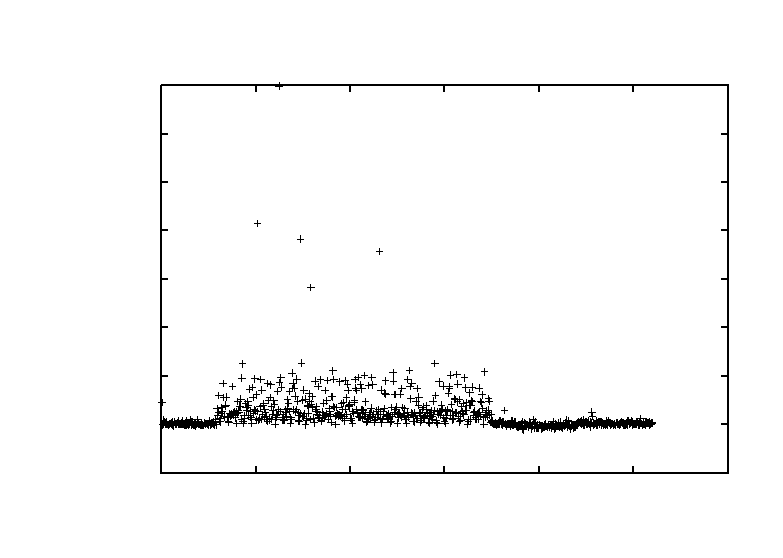
\includegraphics{fig/irqXeno}}%
    \gplfronttext
  \end{picture}%
\endgroup
}}
      \caption{Lat�ncia de interrup��o do Xenomai}
      \label{fig:irqXeno}
    \end{center}
  \end{minipage}
  %\hfill
  \\
  \vspace{.4in}
  \begin{minipage}[!t]{\textwidth}
    \begin{center}  
      \centerline{\resizebox{0.8\linewidth}{!}{% GNUPLOT: LaTeX picture with Postscript
\begingroup
  \makeatletter
  \providecommand\color[2][]{%
    \GenericError{(gnuplot) \space\space\space\@spaces}{%
      Package color not loaded in conjunction with
      terminal option `colourtext'%
    }{See the gnuplot documentation for explanation.%
    }{Either use 'blacktext' in gnuplot or load the package
      color.sty in LaTeX.}%
    \renewcommand\color[2][]{}%
  }%
  \providecommand\includegraphics[2][]{%
    \GenericError{(gnuplot) \space\space\space\@spaces}{%
      Package graphicx or graphics not loaded%
    }{See the gnuplot documentation for explanation.%
    }{The gnuplot epslatex terminal needs graphicx.sty or graphics.sty.}%
    \renewcommand\includegraphics[2][]{}%
  }%
  \providecommand\rotatebox[2]{#2}%
  \@ifundefined{ifGPcolor}{%
    \newif\ifGPcolor
    \GPcolorfalse
  }{}%
  \@ifundefined{ifGPblacktext}{%
    \newif\ifGPblacktext
    \GPblacktextfalse
  }{}%
  % define a \g@addto@macro without @ in the name:
  \let\gplgaddtomacro\g@addto@macro
  % define empty templates for all commands taking text:
  \gdef\gplbacktext{}%
  \gdef\gplfronttext{}%
  \makeatother
  \ifGPblacktext
    % no textcolor at all
    \def\colorrgb#1{}%
    \def\colorgray#1{}%
  \else
    % gray or color?
    \ifGPcolor
      \def\colorrgb#1{\color[rgb]{#1}}%
      \def\colorgray#1{\color[gray]{#1}}%
      \expandafter\def\csname LTw\endcsname{\color{white}}%
      \expandafter\def\csname LTb\endcsname{\color{black}}%
      \expandafter\def\csname LTa\endcsname{\color{black}}%
      \expandafter\def\csname LT0\endcsname{\color[rgb]{1,0,0}}%
      \expandafter\def\csname LT1\endcsname{\color[rgb]{0,1,0}}%
      \expandafter\def\csname LT2\endcsname{\color[rgb]{0,0,1}}%
      \expandafter\def\csname LT3\endcsname{\color[rgb]{1,0,1}}%
      \expandafter\def\csname LT4\endcsname{\color[rgb]{0,1,1}}%
      \expandafter\def\csname LT5\endcsname{\color[rgb]{1,1,0}}%
      \expandafter\def\csname LT6\endcsname{\color[rgb]{0,0,0}}%
      \expandafter\def\csname LT7\endcsname{\color[rgb]{1,0.3,0}}%
      \expandafter\def\csname LT8\endcsname{\color[rgb]{0.5,0.5,0.5}}%
    \else
      % gray
      \def\colorrgb#1{\color{black}}%
      \def\colorgray#1{\color[gray]{#1}}%
      \expandafter\def\csname LTw\endcsname{\color{white}}%
      \expandafter\def\csname LTb\endcsname{\color{black}}%
      \expandafter\def\csname LTa\endcsname{\color{black}}%
      \expandafter\def\csname LT0\endcsname{\color{black}}%
      \expandafter\def\csname LT1\endcsname{\color{black}}%
      \expandafter\def\csname LT2\endcsname{\color{black}}%
      \expandafter\def\csname LT3\endcsname{\color{black}}%
      \expandafter\def\csname LT4\endcsname{\color{black}}%
      \expandafter\def\csname LT5\endcsname{\color{black}}%
      \expandafter\def\csname LT6\endcsname{\color{black}}%
      \expandafter\def\csname LT7\endcsname{\color{black}}%
      \expandafter\def\csname LT8\endcsname{\color{black}}%
    \fi
  \fi
  \setlength{\unitlength}{0.0500bp}%
  \begin{picture}(7200.00,5040.00)%
    \gplgaddtomacro\gplbacktext{%
      \csname LTb\endcsname%
      \put(1254,660){\makebox(0,0)[r]{\strut{}$9.0$}}%
      \put(1254,1125){\makebox(0,0)[r]{\strut{}$9.5$}}%
      \put(1254,1590){\makebox(0,0)[r]{\strut{}$10.0$}}%
      \put(1254,2055){\makebox(0,0)[r]{\strut{}$10.5$}}%
      \put(1254,2520){\makebox(0,0)[r]{\strut{}$11.0$}}%
      \put(1254,2985){\makebox(0,0)[r]{\strut{}$11.5$}}%
      \put(1254,3450){\makebox(0,0)[r]{\strut{}$12.0$}}%
      \put(1254,3915){\makebox(0,0)[r]{\strut{}$12.5$}}%
      \put(1254,4380){\makebox(0,0)[r]{\strut{}$13.0$}}%
      \put(1386,440){\makebox(0,0){\strut{}$ 0$}}%
      \put(2293,440){\makebox(0,0){\strut{}$ 10$}}%
      \put(3199,440){\makebox(0,0){\strut{}$ 20$}}%
      \put(4106,440){\makebox(0,0){\strut{}$ 30$}}%
      \put(5013,440){\makebox(0,0){\strut{}$ 40$}}%
      \put(5919,440){\makebox(0,0){\strut{}$ 50$}}%
      \put(6826,440){\makebox(0,0){\strut{}$ 60$}}%
      \put(220,2520){\rotatebox{90}{\makebox(0,0){\strut{}Lat\^encia em $\mu s$}}}%
      \put(4106,110){\makebox(0,0){\strut{}Tempo de execu\c{c}\~ao em $s$}}%
      \put(4106,4710){\makebox(0,0){\strut{}Xenomai - Lat\^encia de interrup\c{c}\~ao (m�dia)}}%
      \put(5013,3450){\makebox(0,0)[l]{\strut{}Desvio padr\~ao}}%
      \put(5013,3230){\makebox(0,0)[l]{\strut{}m\'{a}ximo 5.2}}%
    }%
    \gplgaddtomacro\gplfronttext{%
    }%
    \gplbacktext
    \put(0,0){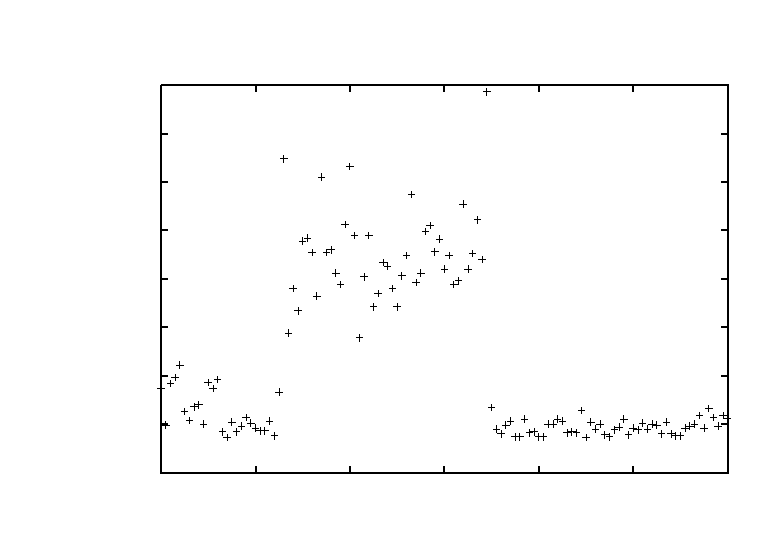
\includegraphics{fig/irqXenoMean}}%
    \gplfronttext
  \end{picture}%
\endgroup
}}
      \caption{Lat�ncia de interrup��o do Xenomai (m�dia sobre 10 valores)}
      \label{fig:irqXenoMean}
    \end{center}
  \end{minipage}
  %\hfill
\end{figure}

\begin{figure}[hbt]
  \index{fig!irqXeno}
  \centering
  % GNUPLOT: LaTeX picture with Postscript
\begingroup
  \makeatletter
  \providecommand\color[2][]{%
    \GenericError{(gnuplot) \space\space\space\@spaces}{%
      Package color not loaded in conjunction with
      terminal option `colourtext'%
    }{See the gnuplot documentation for explanation.%
    }{Either use 'blacktext' in gnuplot or load the package
      color.sty in LaTeX.}%
    \renewcommand\color[2][]{}%
  }%
  \providecommand\includegraphics[2][]{%
    \GenericError{(gnuplot) \space\space\space\@spaces}{%
      Package graphicx or graphics not loaded%
    }{See the gnuplot documentation for explanation.%
    }{The gnuplot epslatex terminal needs graphicx.sty or graphics.sty.}%
    \renewcommand\includegraphics[2][]{}%
  }%
  \providecommand\rotatebox[2]{#2}%
  \@ifundefined{ifGPcolor}{%
    \newif\ifGPcolor
    \GPcolorfalse
  }{}%
  \@ifundefined{ifGPblacktext}{%
    \newif\ifGPblacktext
    \GPblacktextfalse
  }{}%
  % define a \g@addto@macro without @ in the name:
  \let\gplgaddtomacro\g@addto@macro
  % define empty templates for all commands taking text:
  \gdef\gplbacktext{}%
  \gdef\gplfronttext{}%
  \makeatother
  \ifGPblacktext
    % no textcolor at all
    \def\colorrgb#1{}%
    \def\colorgray#1{}%
  \else
    % gray or color?
    \ifGPcolor
      \def\colorrgb#1{\color[rgb]{#1}}%
      \def\colorgray#1{\color[gray]{#1}}%
      \expandafter\def\csname LTw\endcsname{\color{white}}%
      \expandafter\def\csname LTb\endcsname{\color{black}}%
      \expandafter\def\csname LTa\endcsname{\color{black}}%
      \expandafter\def\csname LT0\endcsname{\color[rgb]{1,0,0}}%
      \expandafter\def\csname LT1\endcsname{\color[rgb]{0,1,0}}%
      \expandafter\def\csname LT2\endcsname{\color[rgb]{0,0,1}}%
      \expandafter\def\csname LT3\endcsname{\color[rgb]{1,0,1}}%
      \expandafter\def\csname LT4\endcsname{\color[rgb]{0,1,1}}%
      \expandafter\def\csname LT5\endcsname{\color[rgb]{1,1,0}}%
      \expandafter\def\csname LT6\endcsname{\color[rgb]{0,0,0}}%
      \expandafter\def\csname LT7\endcsname{\color[rgb]{1,0.3,0}}%
      \expandafter\def\csname LT8\endcsname{\color[rgb]{0.5,0.5,0.5}}%
    \else
      % gray
      \def\colorrgb#1{\color{black}}%
      \def\colorgray#1{\color[gray]{#1}}%
      \expandafter\def\csname LTw\endcsname{\color{white}}%
      \expandafter\def\csname LTb\endcsname{\color{black}}%
      \expandafter\def\csname LTa\endcsname{\color{black}}%
      \expandafter\def\csname LT0\endcsname{\color{black}}%
      \expandafter\def\csname LT1\endcsname{\color{black}}%
      \expandafter\def\csname LT2\endcsname{\color{black}}%
      \expandafter\def\csname LT3\endcsname{\color{black}}%
      \expandafter\def\csname LT4\endcsname{\color{black}}%
      \expandafter\def\csname LT5\endcsname{\color{black}}%
      \expandafter\def\csname LT6\endcsname{\color{black}}%
      \expandafter\def\csname LT7\endcsname{\color{black}}%
      \expandafter\def\csname LT8\endcsname{\color{black}}%
    \fi
  \fi
  \setlength{\unitlength}{0.0500bp}%
  \begin{picture}(7200.00,5040.00)%
    \gplgaddtomacro\gplbacktext{%
      \csname LTb\endcsname%
      \put(1254,660){\makebox(0,0)[r]{\strut{}$5.0$}}%
      \put(1254,1125){\makebox(0,0)[r]{\strut{}$10.0$}}%
      \put(1254,1590){\makebox(0,0)[r]{\strut{}$15.0$}}%
      \put(1254,2055){\makebox(0,0)[r]{\strut{}$20.0$}}%
      \put(1254,2520){\makebox(0,0)[r]{\strut{}$25.0$}}%
      \put(1254,2985){\makebox(0,0)[r]{\strut{}$30.0$}}%
      \put(1254,3450){\makebox(0,0)[r]{\strut{}$35.0$}}%
      \put(1254,3915){\makebox(0,0)[r]{\strut{}$40.0$}}%
      \put(1254,4380){\makebox(0,0)[r]{\strut{}$45.0$}}%
      \put(1386,440){\makebox(0,0){\strut{}$ 0$}}%
      \put(2293,440){\makebox(0,0){\strut{}$ 10$}}%
      \put(3199,440){\makebox(0,0){\strut{}$ 20$}}%
      \put(4106,440){\makebox(0,0){\strut{}$ 30$}}%
      \put(5013,440){\makebox(0,0){\strut{}$ 40$}}%
      \put(5919,440){\makebox(0,0){\strut{}$ 50$}}%
      \put(6826,440){\makebox(0,0){\strut{}$ 60$}}%
      \put(220,2520){\rotatebox{90}{\makebox(0,0){\strut{}Lat\^encia em $\mu s$}}}%
      \put(4106,110){\makebox(0,0){\strut{}Tempo de execu\c{c}\~ao em $s$}}%
      \put(4106,4710){\makebox(0,0){\strut{}Xenomai - Lat\^encia de interrup\c{c}\~ao}}%
    }%
    \gplgaddtomacro\gplfronttext{%
    }%
    \gplbacktext
    \put(0,0){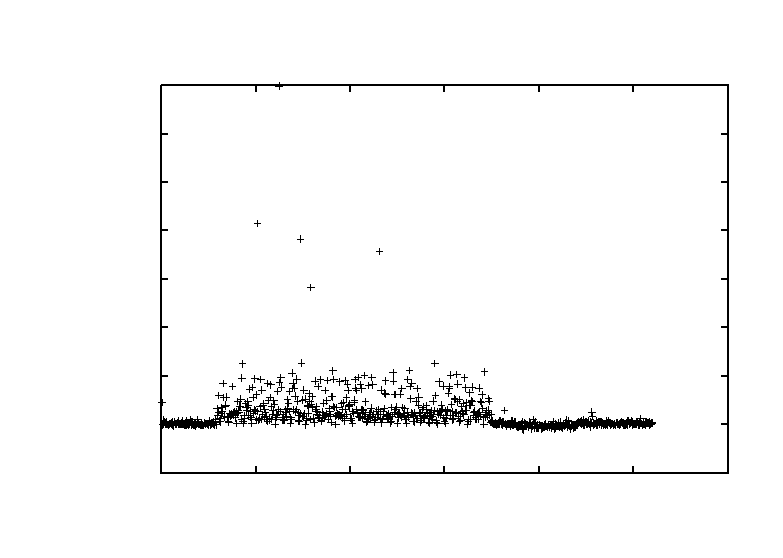
\includegraphics{fig/irqXeno}}%
    \gplfronttext
  \end{picture}%
\endgroup

  \caption{Lat�ncia de interrup��o do Xenomai}
  \label{fig:irqXeno}
\end{figure}

\begin{figure}[hbt]
  \index{fig!irqXenoMean}
  \centering
  % GNUPLOT: LaTeX picture with Postscript
\begingroup
  \makeatletter
  \providecommand\color[2][]{%
    \GenericError{(gnuplot) \space\space\space\@spaces}{%
      Package color not loaded in conjunction with
      terminal option `colourtext'%
    }{See the gnuplot documentation for explanation.%
    }{Either use 'blacktext' in gnuplot or load the package
      color.sty in LaTeX.}%
    \renewcommand\color[2][]{}%
  }%
  \providecommand\includegraphics[2][]{%
    \GenericError{(gnuplot) \space\space\space\@spaces}{%
      Package graphicx or graphics not loaded%
    }{See the gnuplot documentation for explanation.%
    }{The gnuplot epslatex terminal needs graphicx.sty or graphics.sty.}%
    \renewcommand\includegraphics[2][]{}%
  }%
  \providecommand\rotatebox[2]{#2}%
  \@ifundefined{ifGPcolor}{%
    \newif\ifGPcolor
    \GPcolorfalse
  }{}%
  \@ifundefined{ifGPblacktext}{%
    \newif\ifGPblacktext
    \GPblacktextfalse
  }{}%
  % define a \g@addto@macro without @ in the name:
  \let\gplgaddtomacro\g@addto@macro
  % define empty templates for all commands taking text:
  \gdef\gplbacktext{}%
  \gdef\gplfronttext{}%
  \makeatother
  \ifGPblacktext
    % no textcolor at all
    \def\colorrgb#1{}%
    \def\colorgray#1{}%
  \else
    % gray or color?
    \ifGPcolor
      \def\colorrgb#1{\color[rgb]{#1}}%
      \def\colorgray#1{\color[gray]{#1}}%
      \expandafter\def\csname LTw\endcsname{\color{white}}%
      \expandafter\def\csname LTb\endcsname{\color{black}}%
      \expandafter\def\csname LTa\endcsname{\color{black}}%
      \expandafter\def\csname LT0\endcsname{\color[rgb]{1,0,0}}%
      \expandafter\def\csname LT1\endcsname{\color[rgb]{0,1,0}}%
      \expandafter\def\csname LT2\endcsname{\color[rgb]{0,0,1}}%
      \expandafter\def\csname LT3\endcsname{\color[rgb]{1,0,1}}%
      \expandafter\def\csname LT4\endcsname{\color[rgb]{0,1,1}}%
      \expandafter\def\csname LT5\endcsname{\color[rgb]{1,1,0}}%
      \expandafter\def\csname LT6\endcsname{\color[rgb]{0,0,0}}%
      \expandafter\def\csname LT7\endcsname{\color[rgb]{1,0.3,0}}%
      \expandafter\def\csname LT8\endcsname{\color[rgb]{0.5,0.5,0.5}}%
    \else
      % gray
      \def\colorrgb#1{\color{black}}%
      \def\colorgray#1{\color[gray]{#1}}%
      \expandafter\def\csname LTw\endcsname{\color{white}}%
      \expandafter\def\csname LTb\endcsname{\color{black}}%
      \expandafter\def\csname LTa\endcsname{\color{black}}%
      \expandafter\def\csname LT0\endcsname{\color{black}}%
      \expandafter\def\csname LT1\endcsname{\color{black}}%
      \expandafter\def\csname LT2\endcsname{\color{black}}%
      \expandafter\def\csname LT3\endcsname{\color{black}}%
      \expandafter\def\csname LT4\endcsname{\color{black}}%
      \expandafter\def\csname LT5\endcsname{\color{black}}%
      \expandafter\def\csname LT6\endcsname{\color{black}}%
      \expandafter\def\csname LT7\endcsname{\color{black}}%
      \expandafter\def\csname LT8\endcsname{\color{black}}%
    \fi
  \fi
  \setlength{\unitlength}{0.0500bp}%
  \begin{picture}(7200.00,5040.00)%
    \gplgaddtomacro\gplbacktext{%
      \csname LTb\endcsname%
      \put(1254,660){\makebox(0,0)[r]{\strut{}$9.0$}}%
      \put(1254,1125){\makebox(0,0)[r]{\strut{}$9.5$}}%
      \put(1254,1590){\makebox(0,0)[r]{\strut{}$10.0$}}%
      \put(1254,2055){\makebox(0,0)[r]{\strut{}$10.5$}}%
      \put(1254,2520){\makebox(0,0)[r]{\strut{}$11.0$}}%
      \put(1254,2985){\makebox(0,0)[r]{\strut{}$11.5$}}%
      \put(1254,3450){\makebox(0,0)[r]{\strut{}$12.0$}}%
      \put(1254,3915){\makebox(0,0)[r]{\strut{}$12.5$}}%
      \put(1254,4380){\makebox(0,0)[r]{\strut{}$13.0$}}%
      \put(1386,440){\makebox(0,0){\strut{}$ 0$}}%
      \put(2293,440){\makebox(0,0){\strut{}$ 10$}}%
      \put(3199,440){\makebox(0,0){\strut{}$ 20$}}%
      \put(4106,440){\makebox(0,0){\strut{}$ 30$}}%
      \put(5013,440){\makebox(0,0){\strut{}$ 40$}}%
      \put(5919,440){\makebox(0,0){\strut{}$ 50$}}%
      \put(6826,440){\makebox(0,0){\strut{}$ 60$}}%
      \put(220,2520){\rotatebox{90}{\makebox(0,0){\strut{}Lat\^encia em $\mu s$}}}%
      \put(4106,110){\makebox(0,0){\strut{}Tempo de execu\c{c}\~ao em $s$}}%
      \put(4106,4710){\makebox(0,0){\strut{}Xenomai - Lat\^encia de interrup\c{c}\~ao (m�dia)}}%
      \put(5013,3450){\makebox(0,0)[l]{\strut{}Desvio padr\~ao}}%
      \put(5013,3230){\makebox(0,0)[l]{\strut{}m\'{a}ximo 5.2}}%
    }%
    \gplgaddtomacro\gplfronttext{%
    }%
    \gplbacktext
    \put(0,0){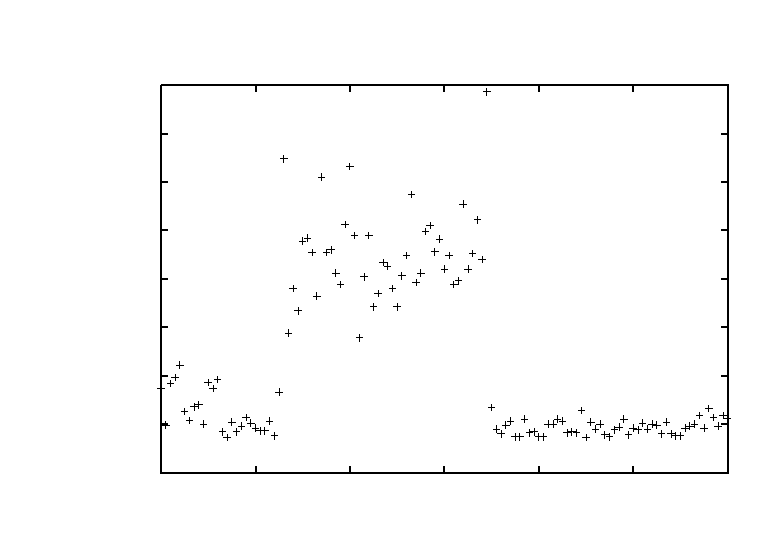
\includegraphics{fig/irqXenoMean}}%
    \gplfronttext
  \end{picture}%
\endgroup

  \caption{Lat�ncia de interrup��o do Xenomai  (m�dia sobre 10 valores)}
  \label{fig:irqXenoMean}
\end{figure}

\begin{figure}[hbt]
  \index{fig!irqRTAI}
  \centering
  % GNUPLOT: LaTeX picture with Postscript
\begingroup
  \makeatletter
  \providecommand\color[2][]{%
    \GenericError{(gnuplot) \space\space\space\@spaces}{%
      Package color not loaded in conjunction with
      terminal option `colourtext'%
    }{See the gnuplot documentation for explanation.%
    }{Either use 'blacktext' in gnuplot or load the package
      color.sty in LaTeX.}%
    \renewcommand\color[2][]{}%
  }%
  \providecommand\includegraphics[2][]{%
    \GenericError{(gnuplot) \space\space\space\@spaces}{%
      Package graphicx or graphics not loaded%
    }{See the gnuplot documentation for explanation.%
    }{The gnuplot epslatex terminal needs graphicx.sty or graphics.sty.}%
    \renewcommand\includegraphics[2][]{}%
  }%
  \providecommand\rotatebox[2]{#2}%
  \@ifundefined{ifGPcolor}{%
    \newif\ifGPcolor
    \GPcolorfalse
  }{}%
  \@ifundefined{ifGPblacktext}{%
    \newif\ifGPblacktext
    \GPblacktextfalse
  }{}%
  % define a \g@addto@macro without @ in the name:
  \let\gplgaddtomacro\g@addto@macro
  % define empty templates for all commands taking text:
  \gdef\gplbacktext{}%
  \gdef\gplfronttext{}%
  \makeatother
  \ifGPblacktext
    % no textcolor at all
    \def\colorrgb#1{}%
    \def\colorgray#1{}%
  \else
    % gray or color?
    \ifGPcolor
      \def\colorrgb#1{\color[rgb]{#1}}%
      \def\colorgray#1{\color[gray]{#1}}%
      \expandafter\def\csname LTw\endcsname{\color{white}}%
      \expandafter\def\csname LTb\endcsname{\color{black}}%
      \expandafter\def\csname LTa\endcsname{\color{black}}%
      \expandafter\def\csname LT0\endcsname{\color[rgb]{1,0,0}}%
      \expandafter\def\csname LT1\endcsname{\color[rgb]{0,1,0}}%
      \expandafter\def\csname LT2\endcsname{\color[rgb]{0,0,1}}%
      \expandafter\def\csname LT3\endcsname{\color[rgb]{1,0,1}}%
      \expandafter\def\csname LT4\endcsname{\color[rgb]{0,1,1}}%
      \expandafter\def\csname LT5\endcsname{\color[rgb]{1,1,0}}%
      \expandafter\def\csname LT6\endcsname{\color[rgb]{0,0,0}}%
      \expandafter\def\csname LT7\endcsname{\color[rgb]{1,0.3,0}}%
      \expandafter\def\csname LT8\endcsname{\color[rgb]{0.5,0.5,0.5}}%
    \else
      % gray
      \def\colorrgb#1{\color{black}}%
      \def\colorgray#1{\color[gray]{#1}}%
      \expandafter\def\csname LTw\endcsname{\color{white}}%
      \expandafter\def\csname LTb\endcsname{\color{black}}%
      \expandafter\def\csname LTa\endcsname{\color{black}}%
      \expandafter\def\csname LT0\endcsname{\color{black}}%
      \expandafter\def\csname LT1\endcsname{\color{black}}%
      \expandafter\def\csname LT2\endcsname{\color{black}}%
      \expandafter\def\csname LT3\endcsname{\color{black}}%
      \expandafter\def\csname LT4\endcsname{\color{black}}%
      \expandafter\def\csname LT5\endcsname{\color{black}}%
      \expandafter\def\csname LT6\endcsname{\color{black}}%
      \expandafter\def\csname LT7\endcsname{\color{black}}%
      \expandafter\def\csname LT8\endcsname{\color{black}}%
    \fi
  \fi
  \setlength{\unitlength}{0.0500bp}%
  \begin{picture}(7200.00,5040.00)%
    \gplgaddtomacro\gplbacktext{%
      \csname LTb\endcsname%
      \put(1254,660){\makebox(0,0)[r]{\strut{}$0.0$}}%
      \put(1254,1125){\makebox(0,0)[r]{\strut{}$10.0$}}%
      \put(1254,1590){\makebox(0,0)[r]{\strut{}$20.0$}}%
      \put(1254,2055){\makebox(0,0)[r]{\strut{}$30.0$}}%
      \put(1254,2520){\makebox(0,0)[r]{\strut{}$40.0$}}%
      \put(1254,2985){\makebox(0,0)[r]{\strut{}$50.0$}}%
      \put(1254,3450){\makebox(0,0)[r]{\strut{}$60.0$}}%
      \put(1254,3915){\makebox(0,0)[r]{\strut{}$70.0$}}%
      \put(1254,4380){\makebox(0,0)[r]{\strut{}$80.0$}}%
      \put(1386,440){\makebox(0,0){\strut{}$ 0$}}%
      \put(1990,440){\makebox(0,0){\strut{}$ 5$}}%
      \put(2595,440){\makebox(0,0){\strut{}$ 10$}}%
      \put(3199,440){\makebox(0,0){\strut{}$ 15$}}%
      \put(3804,440){\makebox(0,0){\strut{}$ 20$}}%
      \put(4408,440){\makebox(0,0){\strut{}$ 25$}}%
      \put(5013,440){\makebox(0,0){\strut{}$ 30$}}%
      \put(5617,440){\makebox(0,0){\strut{}$ 35$}}%
      \put(6222,440){\makebox(0,0){\strut{}$ 40$}}%
      \put(6826,440){\makebox(0,0){\strut{}$ 45$}}%
      \put(220,2520){\rotatebox{90}{\makebox(0,0){\strut{}Lat\^encia em $\mu s$}}}%
      \put(4106,110){\makebox(0,0){\strut{}Tempo de execu\c{c}\~ao em $s$}}%
      \put(4106,4710){\makebox(0,0){\strut{}RTAI - Lat\^encia de interrup\c{c}\~ao}}%
    }%
    \gplgaddtomacro\gplfronttext{%
    }%
    \gplbacktext
    \put(0,0){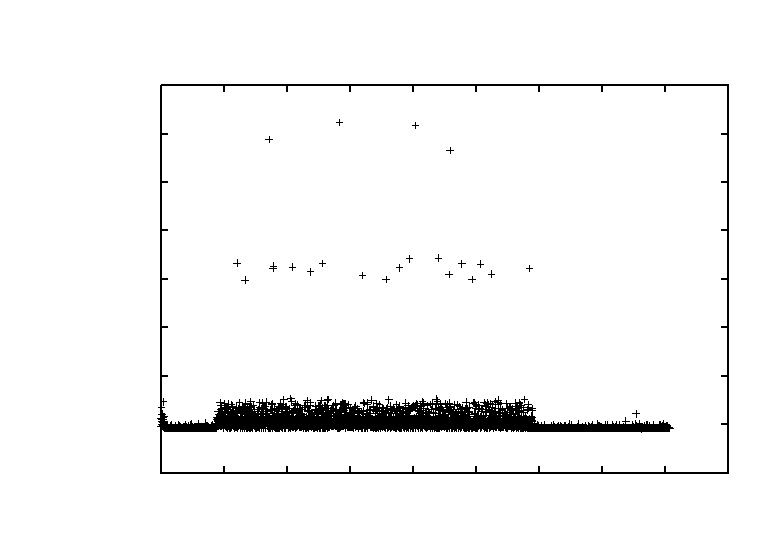
\includegraphics{fig/irqRTAI}}%
    \gplfronttext
  \end{picture}%
\endgroup

  \caption{Lat�ncia de interrup��o do RTAI}
  \label{fig:irqRTAI}
\end{figure}




  \begin{figure}
    \begin{center}
      % GNUPLOT: LaTeX picture with Postscript
\begingroup
  \makeatletter
  \providecommand\color[2][]{%
    \GenericError{(gnuplot) \space\space\space\@spaces}{%
      Package color not loaded in conjunction with
      terminal option `colourtext'%
    }{See the gnuplot documentation for explanation.%
    }{Either use 'blacktext' in gnuplot or load the package
      color.sty in LaTeX.}%
    \renewcommand\color[2][]{}%
  }%
  \providecommand\includegraphics[2][]{%
    \GenericError{(gnuplot) \space\space\space\@spaces}{%
      Package graphicx or graphics not loaded%
    }{See the gnuplot documentation for explanation.%
    }{The gnuplot epslatex terminal needs graphicx.sty or graphics.sty.}%
    \renewcommand\includegraphics[2][]{}%
  }%
  \providecommand\rotatebox[2]{#2}%
  \@ifundefined{ifGPcolor}{%
    \newif\ifGPcolor
    \GPcolorfalse
  }{}%
  \@ifundefined{ifGPblacktext}{%
    \newif\ifGPblacktext
    \GPblacktextfalse
  }{}%
  % define a \g@addto@macro without @ in the name:
  \let\gplgaddtomacro\g@addto@macro
  % define empty templates for all commands taking text:
  \gdef\gplbacktext{}%
  \gdef\gplfronttext{}%
  \makeatother
  \ifGPblacktext
    % no textcolor at all
    \def\colorrgb#1{}%
    \def\colorgray#1{}%
  \else
    % gray or color?
    \ifGPcolor
      \def\colorrgb#1{\color[rgb]{#1}}%
      \def\colorgray#1{\color[gray]{#1}}%
      \expandafter\def\csname LTw\endcsname{\color{white}}%
      \expandafter\def\csname LTb\endcsname{\color{black}}%
      \expandafter\def\csname LTa\endcsname{\color{black}}%
      \expandafter\def\csname LT0\endcsname{\color[rgb]{1,0,0}}%
      \expandafter\def\csname LT1\endcsname{\color[rgb]{0,1,0}}%
      \expandafter\def\csname LT2\endcsname{\color[rgb]{0,0,1}}%
      \expandafter\def\csname LT3\endcsname{\color[rgb]{1,0,1}}%
      \expandafter\def\csname LT4\endcsname{\color[rgb]{0,1,1}}%
      \expandafter\def\csname LT5\endcsname{\color[rgb]{1,1,0}}%
      \expandafter\def\csname LT6\endcsname{\color[rgb]{0,0,0}}%
      \expandafter\def\csname LT7\endcsname{\color[rgb]{1,0.3,0}}%
      \expandafter\def\csname LT8\endcsname{\color[rgb]{0.5,0.5,0.5}}%
    \else
      % gray
      \def\colorrgb#1{\color{black}}%
      \def\colorgray#1{\color[gray]{#1}}%
      \expandafter\def\csname LTw\endcsname{\color{white}}%
      \expandafter\def\csname LTb\endcsname{\color{black}}%
      \expandafter\def\csname LTa\endcsname{\color{black}}%
      \expandafter\def\csname LT0\endcsname{\color{black}}%
      \expandafter\def\csname LT1\endcsname{\color{black}}%
      \expandafter\def\csname LT2\endcsname{\color{black}}%
      \expandafter\def\csname LT3\endcsname{\color{black}}%
      \expandafter\def\csname LT4\endcsname{\color{black}}%
      \expandafter\def\csname LT5\endcsname{\color{black}}%
      \expandafter\def\csname LT6\endcsname{\color{black}}%
      \expandafter\def\csname LT7\endcsname{\color{black}}%
      \expandafter\def\csname LT8\endcsname{\color{black}}%
    \fi
  \fi
  \setlength{\unitlength}{0.0500bp}%
  \begin{picture}(7200.00,5040.00)%
    \gplgaddtomacro\gplbacktext{%
      \csname LTb\endcsname%
      \put(1386,660){\makebox(0,0)[r]{\strut{}$295.0$}}%
      \put(1386,1032){\makebox(0,0)[r]{\strut{}$296.0$}}%
      \put(1386,1404){\makebox(0,0)[r]{\strut{}$297.0$}}%
      \put(1386,1776){\makebox(0,0)[r]{\strut{}$298.0$}}%
      \put(1386,2148){\makebox(0,0)[r]{\strut{}$299.0$}}%
      \put(1386,2520){\makebox(0,0)[r]{\strut{}$300.0$}}%
      \put(1386,2892){\makebox(0,0)[r]{\strut{}$301.0$}}%
      \put(1386,3264){\makebox(0,0)[r]{\strut{}$302.0$}}%
      \put(1386,3636){\makebox(0,0)[r]{\strut{}$303.0$}}%
      \put(1386,4008){\makebox(0,0)[r]{\strut{}$304.0$}}%
      \put(1386,4380){\makebox(0,0)[r]{\strut{}$305.0$}}%
      \put(1518,440){\makebox(0,0){\strut{}$ 0$}}%
      \put(2276,440){\makebox(0,0){\strut{}$ 10$}}%
      \put(3035,440){\makebox(0,0){\strut{}$ 20$}}%
      \put(3793,440){\makebox(0,0){\strut{}$ 30$}}%
      \put(4551,440){\makebox(0,0){\strut{}$ 40$}}%
      \put(5309,440){\makebox(0,0){\strut{}$ 50$}}%
      \put(6068,440){\makebox(0,0){\strut{}$ 60$}}%
      \put(6826,440){\makebox(0,0){\strut{}$ 70$}}%
      \put(220,2520){\rotatebox{90}{\makebox(0,0){\strut{}Lat\^encia em $\mu s$}}}%
      \put(4172,110){\makebox(0,0){\strut{}Tempo de execu\c{c}\~ao em $s$}}%
      \put(4172,4710){\makebox(0,0){\strut{}Xenomai sem estresse, com ajusto - Lat\^encia de escalonamento}}%
    }%
    \gplgaddtomacro\gplfronttext{%
    }%
    \gplbacktext
    \put(0,0){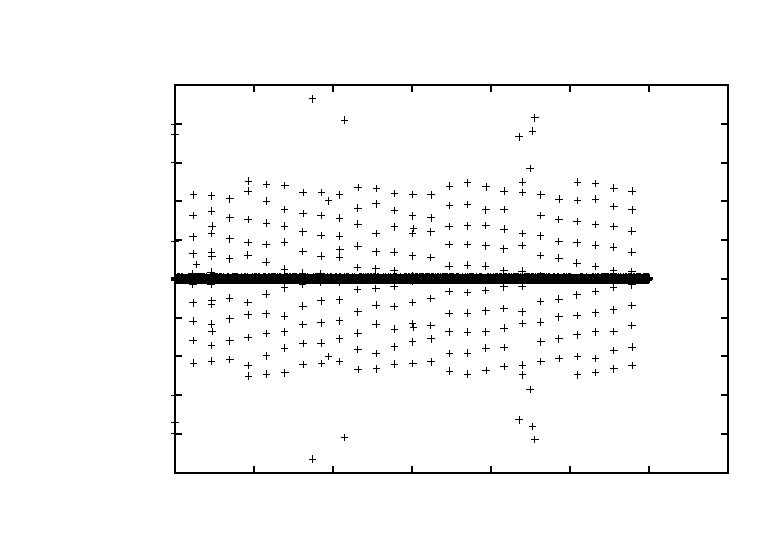
\includegraphics{fig/realSemStr}}%
    \gplfronttext
  \end{picture}%
\endgroup

    \end{center}
  \end{figure}

  \begin{figure}
    \begin{center}
      % GNUPLOT: LaTeX picture with Postscript
\begingroup
  \makeatletter
  \providecommand\color[2][]{%
    \GenericError{(gnuplot) \space\space\space\@spaces}{%
      Package color not loaded in conjunction with
      terminal option `colourtext'%
    }{See the gnuplot documentation for explanation.%
    }{Either use 'blacktext' in gnuplot or load the package
      color.sty in LaTeX.}%
    \renewcommand\color[2][]{}%
  }%
  \providecommand\includegraphics[2][]{%
    \GenericError{(gnuplot) \space\space\space\@spaces}{%
      Package graphicx or graphics not loaded%
    }{See the gnuplot documentation for explanation.%
    }{The gnuplot epslatex terminal needs graphicx.sty or graphics.sty.}%
    \renewcommand\includegraphics[2][]{}%
  }%
  \providecommand\rotatebox[2]{#2}%
  \@ifundefined{ifGPcolor}{%
    \newif\ifGPcolor
    \GPcolorfalse
  }{}%
  \@ifundefined{ifGPblacktext}{%
    \newif\ifGPblacktext
    \GPblacktextfalse
  }{}%
  % define a \g@addto@macro without @ in the name:
  \let\gplgaddtomacro\g@addto@macro
  % define empty templates for all commands taking text:
  \gdef\gplbacktext{}%
  \gdef\gplfronttext{}%
  \makeatother
  \ifGPblacktext
    % no textcolor at all
    \def\colorrgb#1{}%
    \def\colorgray#1{}%
  \else
    % gray or color?
    \ifGPcolor
      \def\colorrgb#1{\color[rgb]{#1}}%
      \def\colorgray#1{\color[gray]{#1}}%
      \expandafter\def\csname LTw\endcsname{\color{white}}%
      \expandafter\def\csname LTb\endcsname{\color{black}}%
      \expandafter\def\csname LTa\endcsname{\color{black}}%
      \expandafter\def\csname LT0\endcsname{\color[rgb]{1,0,0}}%
      \expandafter\def\csname LT1\endcsname{\color[rgb]{0,1,0}}%
      \expandafter\def\csname LT2\endcsname{\color[rgb]{0,0,1}}%
      \expandafter\def\csname LT3\endcsname{\color[rgb]{1,0,1}}%
      \expandafter\def\csname LT4\endcsname{\color[rgb]{0,1,1}}%
      \expandafter\def\csname LT5\endcsname{\color[rgb]{1,1,0}}%
      \expandafter\def\csname LT6\endcsname{\color[rgb]{0,0,0}}%
      \expandafter\def\csname LT7\endcsname{\color[rgb]{1,0.3,0}}%
      \expandafter\def\csname LT8\endcsname{\color[rgb]{0.5,0.5,0.5}}%
    \else
      % gray
      \def\colorrgb#1{\color{black}}%
      \def\colorgray#1{\color[gray]{#1}}%
      \expandafter\def\csname LTw\endcsname{\color{white}}%
      \expandafter\def\csname LTb\endcsname{\color{black}}%
      \expandafter\def\csname LTa\endcsname{\color{black}}%
      \expandafter\def\csname LT0\endcsname{\color{black}}%
      \expandafter\def\csname LT1\endcsname{\color{black}}%
      \expandafter\def\csname LT2\endcsname{\color{black}}%
      \expandafter\def\csname LT3\endcsname{\color{black}}%
      \expandafter\def\csname LT4\endcsname{\color{black}}%
      \expandafter\def\csname LT5\endcsname{\color{black}}%
      \expandafter\def\csname LT6\endcsname{\color{black}}%
      \expandafter\def\csname LT7\endcsname{\color{black}}%
      \expandafter\def\csname LT8\endcsname{\color{black}}%
    \fi
  \fi
  \setlength{\unitlength}{0.0500bp}%
  \begin{picture}(7200.00,5040.00)%
    \gplgaddtomacro\gplbacktext{%
      \csname LTb\endcsname%
      \put(1254,660){\makebox(0,0)[r]{\strut{}$-1.0$}}%
      \put(1254,1125){\makebox(0,0)[r]{\strut{}$0.0$}}%
      \put(1254,1590){\makebox(0,0)[r]{\strut{}$1.0$}}%
      \put(1254,2055){\makebox(0,0)[r]{\strut{}$2.0$}}%
      \put(1254,2520){\makebox(0,0)[r]{\strut{}$3.0$}}%
      \put(1254,2985){\makebox(0,0)[r]{\strut{}$4.0$}}%
      \put(1254,3450){\makebox(0,0)[r]{\strut{}$5.0$}}%
      \put(1254,3915){\makebox(0,0)[r]{\strut{}$6.0$}}%
      \put(1254,4380){\makebox(0,0)[r]{\strut{}$7.0$}}%
      \put(1386,440){\makebox(0,0){\strut{}$ 0$}}%
      \put(2163,440){\makebox(0,0){\strut{}$ 10$}}%
      \put(2940,440){\makebox(0,0){\strut{}$ 20$}}%
      \put(3717,440){\makebox(0,0){\strut{}$ 30$}}%
      \put(4495,440){\makebox(0,0){\strut{}$ 40$}}%
      \put(5272,440){\makebox(0,0){\strut{}$ 50$}}%
      \put(6049,440){\makebox(0,0){\strut{}$ 60$}}%
      \put(6826,440){\makebox(0,0){\strut{}$ 70$}}%
      \put(220,2520){\rotatebox{90}{\makebox(0,0){\strut{}Lat\^encia em $\mu s$}}}%
      \put(4106,110){\makebox(0,0){\strut{}Tempo de execu\c{c}\~ao em $s$}}%
      \put(4106,4710){\makebox(0,0){\strut{}Xenomai sem estresse, com ajusto - Lat\^encia de escalonamento}}%
    }%
    \gplgaddtomacro\gplfronttext{%
    }%
    \gplbacktext
    \put(0,0){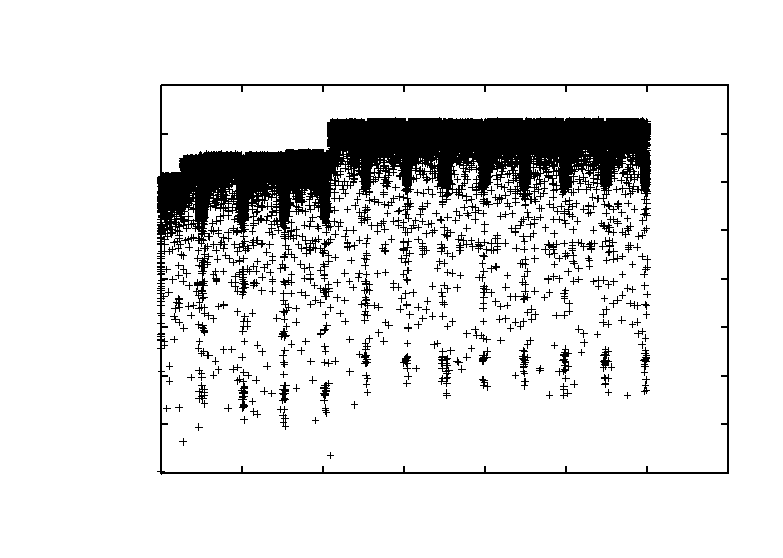
\includegraphics{fig/diffSemStr}}%
    \gplfronttext
  \end{picture}%
\endgroup

    \end{center}
  \end{figure}


  \begin{figure}
    \begin{center}
      % GNUPLOT: LaTeX picture with Postscript
\begingroup
  \makeatletter
  \providecommand\color[2][]{%
    \GenericError{(gnuplot) \space\space\space\@spaces}{%
      Package color not loaded in conjunction with
      terminal option `colourtext'%
    }{See the gnuplot documentation for explanation.%
    }{Either use 'blacktext' in gnuplot or load the package
      color.sty in LaTeX.}%
    \renewcommand\color[2][]{}%
  }%
  \providecommand\includegraphics[2][]{%
    \GenericError{(gnuplot) \space\space\space\@spaces}{%
      Package graphicx or graphics not loaded%
    }{See the gnuplot documentation for explanation.%
    }{The gnuplot epslatex terminal needs graphicx.sty or graphics.sty.}%
    \renewcommand\includegraphics[2][]{}%
  }%
  \providecommand\rotatebox[2]{#2}%
  \@ifundefined{ifGPcolor}{%
    \newif\ifGPcolor
    \GPcolorfalse
  }{}%
  \@ifundefined{ifGPblacktext}{%
    \newif\ifGPblacktext
    \GPblacktextfalse
  }{}%
  % define a \g@addto@macro without @ in the name:
  \let\gplgaddtomacro\g@addto@macro
  % define empty templates for all commands taking text:
  \gdef\gplbacktext{}%
  \gdef\gplfronttext{}%
  \makeatother
  \ifGPblacktext
    % no textcolor at all
    \def\colorrgb#1{}%
    \def\colorgray#1{}%
  \else
    % gray or color?
    \ifGPcolor
      \def\colorrgb#1{\color[rgb]{#1}}%
      \def\colorgray#1{\color[gray]{#1}}%
      \expandafter\def\csname LTw\endcsname{\color{white}}%
      \expandafter\def\csname LTb\endcsname{\color{black}}%
      \expandafter\def\csname LTa\endcsname{\color{black}}%
      \expandafter\def\csname LT0\endcsname{\color[rgb]{1,0,0}}%
      \expandafter\def\csname LT1\endcsname{\color[rgb]{0,1,0}}%
      \expandafter\def\csname LT2\endcsname{\color[rgb]{0,0,1}}%
      \expandafter\def\csname LT3\endcsname{\color[rgb]{1,0,1}}%
      \expandafter\def\csname LT4\endcsname{\color[rgb]{0,1,1}}%
      \expandafter\def\csname LT5\endcsname{\color[rgb]{1,1,0}}%
      \expandafter\def\csname LT6\endcsname{\color[rgb]{0,0,0}}%
      \expandafter\def\csname LT7\endcsname{\color[rgb]{1,0.3,0}}%
      \expandafter\def\csname LT8\endcsname{\color[rgb]{0.5,0.5,0.5}}%
    \else
      % gray
      \def\colorrgb#1{\color{black}}%
      \def\colorgray#1{\color[gray]{#1}}%
      \expandafter\def\csname LTw\endcsname{\color{white}}%
      \expandafter\def\csname LTb\endcsname{\color{black}}%
      \expandafter\def\csname LTa\endcsname{\color{black}}%
      \expandafter\def\csname LT0\endcsname{\color{black}}%
      \expandafter\def\csname LT1\endcsname{\color{black}}%
      \expandafter\def\csname LT2\endcsname{\color{black}}%
      \expandafter\def\csname LT3\endcsname{\color{black}}%
      \expandafter\def\csname LT4\endcsname{\color{black}}%
      \expandafter\def\csname LT5\endcsname{\color{black}}%
      \expandafter\def\csname LT6\endcsname{\color{black}}%
      \expandafter\def\csname LT7\endcsname{\color{black}}%
      \expandafter\def\csname LT8\endcsname{\color{black}}%
    \fi
  \fi
  \setlength{\unitlength}{0.0500bp}%
  \begin{picture}(7200.00,5040.00)%
    \gplgaddtomacro\gplbacktext{%
      \csname LTb\endcsname%
      \put(1386,660){\makebox(0,0)[r]{\strut{}$292.0$}}%
      \put(1386,1125){\makebox(0,0)[r]{\strut{}$294.0$}}%
      \put(1386,1590){\makebox(0,0)[r]{\strut{}$296.0$}}%
      \put(1386,2055){\makebox(0,0)[r]{\strut{}$298.0$}}%
      \put(1386,2520){\makebox(0,0)[r]{\strut{}$300.0$}}%
      \put(1386,2985){\makebox(0,0)[r]{\strut{}$302.0$}}%
      \put(1386,3450){\makebox(0,0)[r]{\strut{}$304.0$}}%
      \put(1386,3915){\makebox(0,0)[r]{\strut{}$306.0$}}%
      \put(1386,4380){\makebox(0,0)[r]{\strut{}$308.0$}}%
      \put(1518,440){\makebox(0,0){\strut{}$ 0$}}%
      \put(2276,440){\makebox(0,0){\strut{}$ 10$}}%
      \put(3035,440){\makebox(0,0){\strut{}$ 20$}}%
      \put(3793,440){\makebox(0,0){\strut{}$ 30$}}%
      \put(4551,440){\makebox(0,0){\strut{}$ 40$}}%
      \put(5309,440){\makebox(0,0){\strut{}$ 50$}}%
      \put(6068,440){\makebox(0,0){\strut{}$ 60$}}%
      \put(6826,440){\makebox(0,0){\strut{}$ 70$}}%
      \put(220,2520){\rotatebox{90}{\makebox(0,0){\strut{}Lat\^encia em $\mu s$}}}%
      \put(4172,110){\makebox(0,0){\strut{}Tempo de execu\c{c}\~ao em $s$}}%
      \put(4172,4710){\makebox(0,0){\strut{}Xenomai com estresse, com ajusto - Lat\^encia de escalonamento}}%
    }%
    \gplgaddtomacro\gplfronttext{%
    }%
    \gplbacktext
    \put(0,0){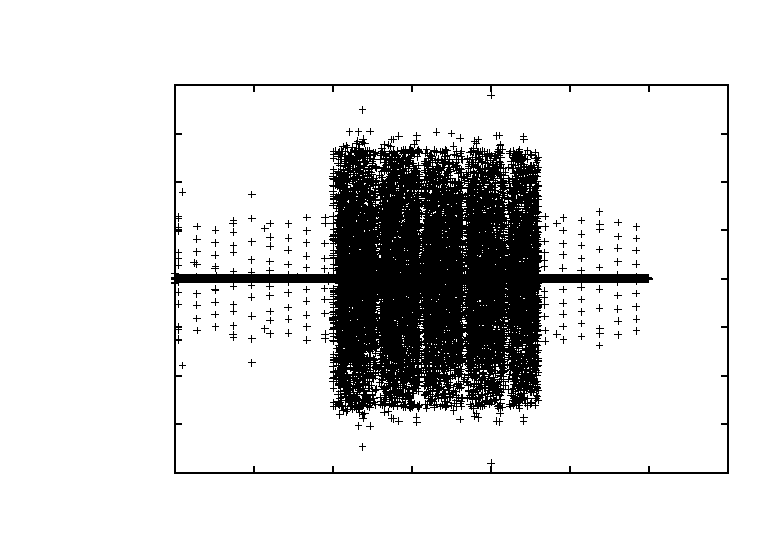
\includegraphics{fig/realComStr}}%
    \gplfronttext
  \end{picture}%
\endgroup

    \end{center}
  \end{figure}

  \begin{figure}
    \begin{center}
      % GNUPLOT: LaTeX picture with Postscript
\begingroup
  \makeatletter
  \providecommand\color[2][]{%
    \GenericError{(gnuplot) \space\space\space\@spaces}{%
      Package color not loaded in conjunction with
      terminal option `colourtext'%
    }{See the gnuplot documentation for explanation.%
    }{Either use 'blacktext' in gnuplot or load the package
      color.sty in LaTeX.}%
    \renewcommand\color[2][]{}%
  }%
  \providecommand\includegraphics[2][]{%
    \GenericError{(gnuplot) \space\space\space\@spaces}{%
      Package graphicx or graphics not loaded%
    }{See the gnuplot documentation for explanation.%
    }{The gnuplot epslatex terminal needs graphicx.sty or graphics.sty.}%
    \renewcommand\includegraphics[2][]{}%
  }%
  \providecommand\rotatebox[2]{#2}%
  \@ifundefined{ifGPcolor}{%
    \newif\ifGPcolor
    \GPcolorfalse
  }{}%
  \@ifundefined{ifGPblacktext}{%
    \newif\ifGPblacktext
    \GPblacktextfalse
  }{}%
  % define a \g@addto@macro without @ in the name:
  \let\gplgaddtomacro\g@addto@macro
  % define empty templates for all commands taking text:
  \gdef\gplbacktext{}%
  \gdef\gplfronttext{}%
  \makeatother
  \ifGPblacktext
    % no textcolor at all
    \def\colorrgb#1{}%
    \def\colorgray#1{}%
  \else
    % gray or color?
    \ifGPcolor
      \def\colorrgb#1{\color[rgb]{#1}}%
      \def\colorgray#1{\color[gray]{#1}}%
      \expandafter\def\csname LTw\endcsname{\color{white}}%
      \expandafter\def\csname LTb\endcsname{\color{black}}%
      \expandafter\def\csname LTa\endcsname{\color{black}}%
      \expandafter\def\csname LT0\endcsname{\color[rgb]{1,0,0}}%
      \expandafter\def\csname LT1\endcsname{\color[rgb]{0,1,0}}%
      \expandafter\def\csname LT2\endcsname{\color[rgb]{0,0,1}}%
      \expandafter\def\csname LT3\endcsname{\color[rgb]{1,0,1}}%
      \expandafter\def\csname LT4\endcsname{\color[rgb]{0,1,1}}%
      \expandafter\def\csname LT5\endcsname{\color[rgb]{1,1,0}}%
      \expandafter\def\csname LT6\endcsname{\color[rgb]{0,0,0}}%
      \expandafter\def\csname LT7\endcsname{\color[rgb]{1,0.3,0}}%
      \expandafter\def\csname LT8\endcsname{\color[rgb]{0.5,0.5,0.5}}%
    \else
      % gray
      \def\colorrgb#1{\color{black}}%
      \def\colorgray#1{\color[gray]{#1}}%
      \expandafter\def\csname LTw\endcsname{\color{white}}%
      \expandafter\def\csname LTb\endcsname{\color{black}}%
      \expandafter\def\csname LTa\endcsname{\color{black}}%
      \expandafter\def\csname LT0\endcsname{\color{black}}%
      \expandafter\def\csname LT1\endcsname{\color{black}}%
      \expandafter\def\csname LT2\endcsname{\color{black}}%
      \expandafter\def\csname LT3\endcsname{\color{black}}%
      \expandafter\def\csname LT4\endcsname{\color{black}}%
      \expandafter\def\csname LT5\endcsname{\color{black}}%
      \expandafter\def\csname LT6\endcsname{\color{black}}%
      \expandafter\def\csname LT7\endcsname{\color{black}}%
      \expandafter\def\csname LT8\endcsname{\color{black}}%
    \fi
  \fi
  \setlength{\unitlength}{0.0500bp}%
  \begin{picture}(7200.00,5040.00)%
    \gplgaddtomacro\gplbacktext{%
      \csname LTb\endcsname%
      \put(1254,660){\makebox(0,0)[r]{\strut{}$-2.0$}}%
      \put(1254,1280){\makebox(0,0)[r]{\strut{}$0.0$}}%
      \put(1254,1900){\makebox(0,0)[r]{\strut{}$2.0$}}%
      \put(1254,2520){\makebox(0,0)[r]{\strut{}$4.0$}}%
      \put(1254,3140){\makebox(0,0)[r]{\strut{}$6.0$}}%
      \put(1254,3760){\makebox(0,0)[r]{\strut{}$8.0$}}%
      \put(1254,4380){\makebox(0,0)[r]{\strut{}$10.0$}}%
      \put(1386,440){\makebox(0,0){\strut{}$ 0$}}%
      \put(2163,440){\makebox(0,0){\strut{}$ 10$}}%
      \put(2940,440){\makebox(0,0){\strut{}$ 20$}}%
      \put(3717,440){\makebox(0,0){\strut{}$ 30$}}%
      \put(4495,440){\makebox(0,0){\strut{}$ 40$}}%
      \put(5272,440){\makebox(0,0){\strut{}$ 50$}}%
      \put(6049,440){\makebox(0,0){\strut{}$ 60$}}%
      \put(6826,440){\makebox(0,0){\strut{}$ 70$}}%
      \put(220,2520){\rotatebox{90}{\makebox(0,0){\strut{}Lat\^encia em $\mu s$}}}%
      \put(4106,110){\makebox(0,0){\strut{}Tempo de execu\c{c}\~ao em $s$}}%
      \put(4106,4710){\makebox(0,0){\strut{}Xenomai com estresse, com ajusto - Lat\^encia de escalonamento}}%
    }%
    \gplgaddtomacro\gplfronttext{%
    }%
    \gplbacktext
    \put(0,0){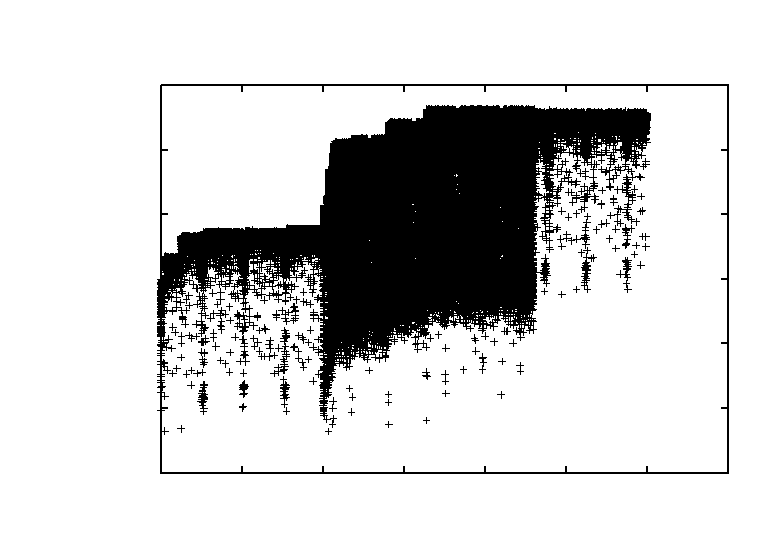
\includegraphics{fig/diffComStr}}%
    \gplfronttext
  \end{picture}%
\endgroup

    \end{center}
  \end{figure}

\end{comment}


\label{ap:doris2}

\end{spacing}

 %%
%% Parte p�s-textual
%%
\backmatter

% Bibliografia
% � aconselh�vel utilizar o BibTeX a partir de um arquivo, digamos "biblio.bib".
% Para ajuda na cria��o do arquivo .bib e utiliza��o do BibTeX, recorra ao
% BibTeXpress em www.cin.ufpe.br/~paguso/bibtexpress
\renewcommand{\bibname}{REFER�NCIAS}
%\nocite{*}
%\bibliographystyle{authordate2}
%\bibliographystyle{abnt-alf}

\bibliography{../../bib}

%% Fim do documento
\end{document}
